\documentclass[12pt,upcase]{mitthesis}

\usepackage{amsmath}
\usepackage{microtype}
\usepackage{graphicx}
\graphicspath{{./images/}}
\usepackage{multirow}
\usepackage{rotating}
\usepackage{natbib}
\usepackage{url}
\usepackage{booktabs}
\usepackage{minted}
\usepackage{scrextend}						% for the labelling list environment used in Ch4
\addtokomafont{labelinglabel}{\sffamily}	% for the labelling list environment used in Ch4

\usepackage[]{pdfpages}

% use fancyhdr, to enable page style stuff (below)
\usepackage{fancyhdr}
\setlength{\headheight}{15.2pt}
\renewcommand{\headrulewidth}{0pt}

\pagestyle{plain}

\begin{document}
% Sherman 1
% Revision 1.1  92/04/22  13:08:20  epeisach

% BE SURE TO READ THE UNIVERSITY'S RULES ON WHAT FIELDS ARE REQUIRED OR ENCOURANGED FOR YOUR DEPARTMENT

\title{Learning Analytics for Block-based Programming: \\ The App Inventor ``Flailing Detector''}

\author{Mark A. Sherman}

\prevdegrees{M.S., University of Massachusets Lowell (2010) \\ B.S., University of Massachusetts Lowell (2008)}

\department{Department of Computer Science}

% If the thesis is for two degrees simultaneously, list them both
% separated by \and like this:
% \degree{Doctor of Philosophy \and Master of Science}
\degree{Doctor of Philosophy}
\degreemonth{December}
\degreeyear{2016}
\thesisdate{November 22, 2016}

% If there is more than one supervisor, use the \supervisor command
% once for each.
\supervisor{Fred G. Martin}{Professor}
\reader{John McCarthy}{Associate Professor}
\reader{Franklyn A. Turbak}{Associate Professor, Wellesley College}

% this is the department committee chairman, not the thesis committee chairman. 
\chairman{Haim Levkowitz}{Department Chairman}

% Make the titlepage based on the above information.  If you need
% something special and can't use the standard form, you can specify
% the exact text of the titlepage yourself.  Put it in a titlepage
% environment and leave blank lines where you want vertical space.
% The spaces will be adjusted to fill the entire page.  The dotted
% lines for the signatures are made with the \signature command.
\maketitle

% The abstractpage environment sets up everything on the page except
% the text itself.  The title and other header material are put at the
% top of the page, and the supervisors are listed at the bottom.  A
% new page is begun both before and after.  Of course, an abstract may
% be more than one page itself.  If you need more control over the
% format of the page, you can use the abstract environment, which puts
% the word "Abstract" at the beginning and single spaces its text.

%% You can either \input (*not* \include) your abstract file, or you can put
%% the text of the abstract directly between the \begin{abstractpage} and
%% \end{abstractpage} commands.

% First copy: start a new page, and save the page number.
\newpage
\thispagestyle{empty}
\mbox{}
\newpage
\thispagestyle{empty}

% Second copy: start a new page, and reset the page number.  This way,
% the second copy of the abstract is not counted as separate pages.
\pagestyle{plain}
\newpage
\setcounter{page}{1}
\pagenumbering{roman}
\begin{abstractpage}


Investigation into students' programming processes has long been a critical area to inform teaching methodology and learning models. Recent technology has created a nascent field of using fine-grained instrumentation---observations of small changes in work over time---to delve into previously inaccessible student behaviors. These behavior data filled in stories that led up to the final program code artifacts; these stories could not be captured by looking at these artifacts alone. 

Also recently, blocks-based programming languages have become popular and practical for pedagogical programming environments. These environments afford new dimensions of learner interaction with code. 

In this work, student progress during a programming challenge activity was investigated. Fine-grained data were collected based on edit operations in students' blocks-programming work. Analysis methods and visualizations for those data were designed and implemented. A construct of a class of behavior called ``flailing'' was developed, and was operationalized to include patterns of repetitive or non-productive changes. This suggested disengagement and potential lack of problem understanding. A simple algorithm was developed to demonstrate that ``flailing'' can be automatically assessed.

In addition to visualizations of individual student progress, a prototype of a classroom ``dashboard'' was developed. This is intended to be used as real-time tool for teachers, to help teachers to assess their students engagement, progress, and degree of flailing during a live lab session. This tool may be helpful to improve teaching effectiveness by aiding in classroom orchestration, empowering the teacher to better employ their resources in the moment, to better keep all students on track.

From these data, three patterns of student were discovered: those who smoothly completed the assignment, those who worked their way through with periods of flailing and periods of success, and those who only flailed and never succeeded. This rating system allowed for the development of a moment-by-moment analysis of flailing, which may provide a real-time assessment of students engagement with the activity, and serve as a tool to further empower the teacher to orchestrate their resources during a lab session.

\end{abstractpage}

%%%%%%%%%%%%%%%%%%%%%%%%%%%%%%%%%%%%%%%%%%%%%%%%%%%%%%%%%%%%%%%%%%%%%%
% -*-latex-*-




\chapter*{Acknowledgments}
\renewcommand{\thefootnote}{\fnsymbol{footnote}}

%TODO

% It is common courtesy to seek permission before listing a person in acknowledgments, so that should be done for all. TODO
Special thanks to Derrell Lipman, Farzeen Harunani, Michael Tissenbaum, Kim Douglas, Molly Laden, Ben Shapiro, Josh Sheldon, Mark Guzdial, Sally Fincher, and Benjamin Xie.

Thank you to my system testers: Mike Staub, William Sokolowsky, Jr., Ambarish Roy, Justin Richer, Charles Kaneb, Nicholas McKinnon, Christian Quale, Joshua Carlson, Russell Bernstein, Allistair Stead, Peter Galvin, Jessica Spink, Tim Baird, Barry Sherman, Emily Jackson, Reed Spool, Caroline Fonseca, Jessica West, Christopher Rogacz, Marybeth Moriarty, Matthew Sherman, and Andrew Chanler.

This material is based upon work supported by the National Science Foundation under Grants DUE-1225719 and DRL-1433592.\footnote{Any opinions, findings, and conclusions or recommendations expressed in this material are those of the author and do not necessarily reflect the views of the National Science Foundation.}

\renewcommand{\thefootnote}{\arabic{footnote}}
  % -*- Mode:TeX -*-
%% This file simply contains the commands that actually generate the table of
%% contents and lists of figures and tables.  You can omit any or all of
%% these files by simply taking out the appropriate command.  For more
%% information on these files, see appendix C.3.3 of the LaTeX manual. 
\tableofcontents
\newpage
\listoffigures
\newpage
\listoftables
\newpage
\listoflistings

%\include{preface} 	% Preface is not part of the standard. I invented it for myself. Use it if you want by uncommenting.

	% Redefine the "plain" pagestyle to have pagenum in the header, right
	\fancypagestyle{plain}{
		\fancyhf{}
		\fancyhead[R]{\thepage}
	}

	\setcounter{page}{1}
	\pagenumbering{arabic}
	\pagestyle{plain}
	
\chapter{Introduction}

\section{Research Focus}
 
\section{Problem Statement}
Let's do a list. Lists are great. The four questions of interest are:
\begin{itemize}
\item Do students exhibit patterns in testing and iteration? What are those patterns?
\item What characteristics of a design activity elicit specific iteration patterns?
\item What is the correlation between iteration in designing and success of the design?
\item What guidelines can be written for the creation of future activities?
\end{itemize}


\section{Approach}

\section{Hypothesis and Contributions}

\section{Rationale}

\chapter{Background}
\label{chap:background}

Previous studies have used fine-grain instrumentation to dive into previously inaccessible student behaviors. These studies varied widely, from the discovery of phases of development over a project \citep{berland-2013, martin2013nanogenetic}, to analysis of off-task behavior in learning \citep{baker2004off}. Some have presented methods for identifying struggling students \cite{piech-2012}, and others develop well-informed assessments \citep{werner2012fairy}. All of them had commonalities: building models of learning by looking at fine-grain behavior data, observing small changes in work over time, filling in the stories that led up to the final artifacts. Examining the process of programming rather than the final products can uncover interesting behavior about student learning, and such patterns may have better predictive power than in-class exams \citep{blikstein2014}.

Analysis of this data was informed by previous studies of student behavior in programming, math, and other activities. \cite{perkins-1986} identified and classified types of behaviors students exhibit when they encounter difficulty in programming. Off-task behavior, to which flailing may be related, has also been studied, such as \cite{baker2004off} did, in the context of mathematics. 

This study relates closely to learning pathways, especially those identified by learning analytics \citep{martin2013nanogenetic}. 

The activities conducted for data collection revolved around debugging, as debugging has been shown to be a compelling mechanism to drive engagement with a short programming task \citep{webb2010troubleshooting}.

A more extensive discussion of related work is presented below.


\section{A Brief History of Learning Theory}
\label{sec:learning-theory}
Piaget, ZPD, etc etc
Also introduce Orchestration
...
Maintaining each students' current position within their zone of proximal development is a critical goal of orchestration, which will be further discussed in Section \ref{sec:teacher-dashboards}.
%TODO this is a stub


\section{Visual Languages}
\label{sec:visual-languages}

Much of the literature concerning programming efficacy was done at a time when visual languages were emerging as a purported panacea of usefulness \citep{shu-1988}, but with little empirical evidence to substantiate those claims \citep{petre-1995}. \citeauthor{sch-1980} made such an accusation, ``Computer scientists... make broad claims for the simplicity, naturalness, or ease-of-use of new computer languages or techniques, but do not take advantage of the opportunity for experimental confirmation'' (\citeyear{sch-1980}). \citeauthor{stefik2014programming} strongly argued that these ``language wars'' are a significant problem to science, and as stewards of computation, it is the language resarchers who must study the imact of language designs on people (\citeyear{stefik2014programming}). Speaking of diagram-based visual languages, \citet{blackwell-2001} offered a challenge to researchers to support their claims of intuition through visual programming, ``...to explain why this intuition may be valid, and to propose the ways in which, if it is valid, it can most be effectively exploited.'' This work hopes to shed some light into the domain illustrated by that challenge. 


\section{App Inventor}
\label{sec:app-inventor-background}
App Inventor is an online development environment to build Android apps, employing a drag-and-drop designer and graphical, blocks-based code editing. App Inventor follows in the tradition of Constructionism \citep{papert1991situating}, which covers a wide class of discovery-based pedagogical vehicles. App Inventor is also deeply influenced by Scratch \citep{resnick2009scratch}, and offers low barriers for entry, high ceilings of capability, and a built-in library of powerful abstractions.

The App Inventor language and runtime uses a purely event-driven programming model, where all functions are driven by events and event handler code \citep{turbak-2014}. The event handlers are separate blocks, and can be organized arbitrarily on the workspace. An example of two event handlers can be seen as the gold, top-level blocks in Figure \ref{fig:debug0ch2}. 

\begin{figure}
  \centering
      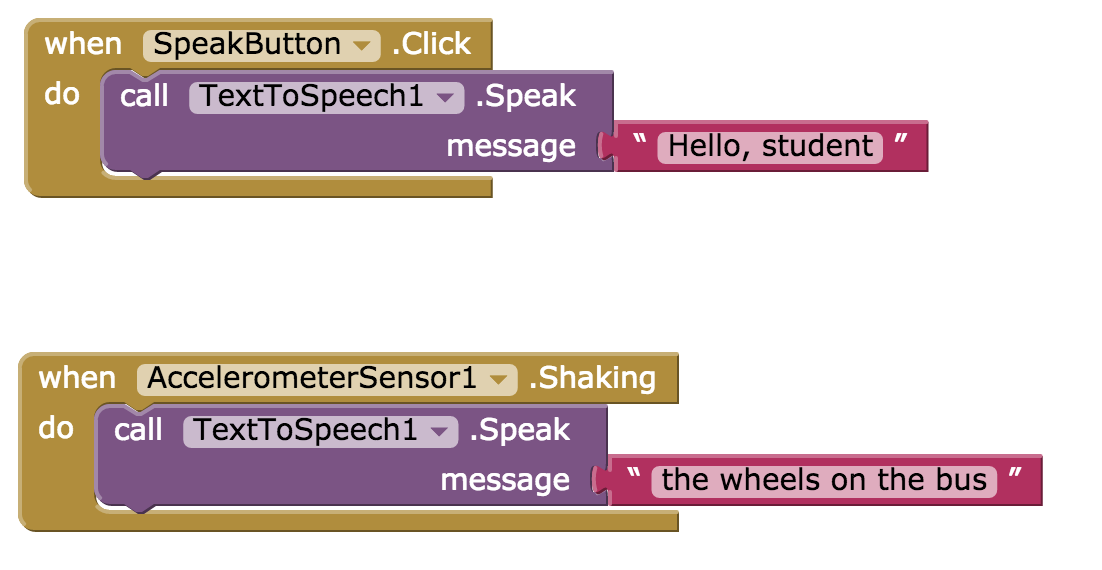
\includegraphics[width=\textwidth]{images/debugActivity/debug0start}
  \caption[Some App Inventor code blocks]{Some App Inventor code blocks. Each gold-colored block is an event handler, which can be arranged arbitrarily on the workspace. The enclosed purple blocks will execute when their parent events are triggered.}
  \label{fig:debug0ch2}
\end{figure}


%\subsection{Cognitive Dimensions of Notations} 
\label{sec:CDs}
The Cognitive Dimensions of Notations framework was developed to provide a vocabulary through which design tools can be assessed and discussed. This framework is suitable for broad evaluation and discussion of how a language suits its users needs. It was developed over many years \citep{green1989cognitive, green1996usability}, and is currently canonized in \citet{blackwell-2003}. Their mission was for this vocabulary to be easily applicable, understandable, and most importantly, be theoretically coherent \citep{petre-2006}. 

%The cognitive dimensions framework presented an empirically-derived set of dimensions that can be generally measured for a given class of user activity. These dimensions described different cognitive mechanisms that are necessary for the user to execute a given action, and helped create a meaningful dialog about how those dimensions can be traded to optimize the action for the user \citep{blackwell-2003}. The research was started to investigate why some notations work and don't work for the people using them \citep{petre-2006}. 

%The dimensions alone do not constitute anything. A dimension is not good or bad. Dimensions are part of the framework's instrument, which includes evaluation of relevant dimensions for a particular task. Application of the the dimensions to a set of representative tasks is what drives the apparatus, and the assessment is in the comparison of the desired dimensionality for those tasks compared to the observed value of those dimensions for the task. This also makes it possible to use the cognitive dimensions framework, in a constrained form, as a user survey tool, to provide users with a method for describing their experience with a notation system.

%Without any further fanfare, here are the dimensions, in their entirety as of \citeyear{blackwell-2003}:
The dimension most critical to this work was \emph{secondary notation,} the information encoded in means other than the formal syntax, primarily in graphical layout. Secondary notation is explored further in Section \ref{sec:secondary-notation} Additionally, \emph{viscosity,} the difficult to make a change, was relevant to this study.

% \begin{description}
% \item [Viscosity] Resistance to change, or difficulty to make a change. Modifying heading styles across a document manually is a viscous activity, in that the user's desired action is seemingly simple, but the effort to execute it is significant.
%\item [Visibility] Ability to view components easily. This dimensions is often traded away in languages in favor of, for example, abstractions.
%\item [Premature commitment] Constraints placed on the order of doing things. In programming, a mechanic of premature commitment forces the programmer to make decisions before they have the information to base the decision on. \citet{roast-2000} described this as "the user having to satisfy the secondary goal prior to achieving the primary goal."
% \item [Hidden dependencies] Entities may cite each other, and a change in one entity may create change elsewhere unexpectedly due ot unapparent citations. This is common in spreadsheets, where cell references are not easily visible.
%\item [Role-expressiveness] The purpose of an entity is readily inferred. The reader can discover the author's intent. 
%\item [Error-proneness] Invites mistakes. Can be protected with preventative mechanisms.  
%\item [Abstractions] Change the underlying notation. Common examples are macros, functions, global find-and-replace, word processor styles, and even speed dial. They can be persistent (macros) or transient (find and replace). An abstraction manager is necessary if the user is allowed to edit the abstractions. 
% \item [Secondary notation] Information encoded in means other than the formal syntax. 
%\item [Closeness of mapping] How closely the notation relates to the result it describes. 
%\item [Consistency] Similar semantics are expressed in similar syntactic forms. Information can be obscured by inconsistent presentation.
%\item [Diffuseness] Verbosity of the language. Large icons, long phrases, and other forms of graphical real estate consumption contribute to diffuseness. I do not know why this dimensions isn't called verbosity, which could easily be contrasted by calling low verbosity succinct.
%\item [Hard mental operations] Creates high demand on cognitive resources. This is an interesting dimension, as it makes clear to designers that sometimes a notation can force a user to work things out in their head, or otherwise tax working memory.
%\item [Provisionality] Provisional notation, meaning temporary, allows for low commitment to a notation. This may be useful for sketching, recording potential options, ``what if'' exercises, and general exploration activities.
%\item [Progressive evaluation] Work can be checked at any time. Evaluation is an important part of the design process, and drives iteration \citep{atman-2003}. A well-known advantage to interpreted programming environments is their ease of work evaluation, where the user can try out partially-completed programs at any time, and have meaningful interactions with their partial work.
% \end{description}


\section{Secondary Notation} %promoted to section for proposal
\label{sec:secondary-notation}
One of these dimensions in particular, secondary notation, emerged as especially important to visual programming \citep{petre-2006}. The work at the time was focused on diagram programming, such as LabVIEW, where researchers found a distinct and repeating signal that differentiated experts from novices. That signal was in the use of secondary notation, where experts would use arrangement and layout of the diagram itself to convey information not encoded in the formal notation. 

Secondary notation is, generally, any notation that's not part of the formal notation, and may include comments and whitespace in text languages, layout in diagrams, proximity in blocks languages, and much more. Often, secondary notation can be used however the user likes, and therefore can be used to record information that the designer of the notation did not anticipate. \citet{petre-1995} claimed that much of the comprehensibility of graphical programming is in the secondary notation, and \citet{raymond-1991} conjectured, even earlier, that the layout of a visual program was the most important, and possibly only, aspect that was truly visual. Of course, \citeauthor{raymond-1991} had a very specific meaning of ``visual,'' where it depended on being non-discrete, unable to guarantee syntactic or semantic differentiation, similar to the mathematical notion of continuity or the electronic notion of analog. In fact, \citeauthor{raymond-1991} called such a language Analog, and contrasted it against Notational languages, which were discrete, with strongly differentiable notational marks and strongly differentiable conceptual objects being represented. This distinction of Notational versus Analog language was developed earlier as part of an interesting philosophical discussion on notations, and asked hard questions about denotation and representation \citep{goodman-1976}. This discussion had nothing to do with programming, nor visual programming, but it was brought into that domain by \citeauthor{raymond-1991}, and nearly predicted the findings of the expert and novice usage difference in secondary notation, found later by \citet{petre-2006}.

Students working in App Inventor have often been observed doing unproductive tinkering, similar to that observed by \citet{perkins-1986}. One hypothesis as to why App Inventor does this can be made with the help of the Cognitive Dimensions Framework \citep{blackwell-2003}. As \citet{petre-2006} observed, experts and novices write and read secondary notation in different ways, and in App Inventor, poor planning of that secondary notation by a novice can result in increased viscosity. Increased viscosity, we hypothesize, may result in tinkering behavior, as it adds time and cognitive load to the user's task. Further investigation along this line is reserved for future work.

\section{Behaviors when Encountering Difficulty}
\label{sec:behaviors}
Novice programmers are faced with a plethora of difficulties to overcome. \citet{perkins-1986} identified some key behavior patterns students may show when they encounter difficulty. To begin, \citeauthor{perkins-1986} observed that most students displayed ``significant powers of invention'' when working with programming tasks, and they employed that inventiveness in tackling problems they encountered. However, there were are an enormous number of pitfalls in the programming process that interfered with that inventiveness leading to a reasonable degree of competence. 

The general behavior patterns that \citet{perkins-1986} identified are as follows. There were two conceptual cohorts: \emph{stoppers} and \emph{movers.} When a stopper found themselves without an immediate answer to a difficulty, they felt at a complete loss, and were unwilling to further explore the problem. They would completely stop working, often sitting back from the computer. This behavior is extremely common, and has been personally observed by the author. A stopper can be rescued with immediate intervention, where a teacher can assess and ask the next questions explicitly (such as ``what do you think that error means?''), and press the student for answers. With this sort of intervention, stoppers usually found a solution for their difficulty, and were able to resume. In the observations of \citeauthor{perkins-1986}, the activities were short, so a rescued stopper could make it successfully to the end of the activity with only one intervention. But that intervention was timely, asserted immediately when the student stopped progressing, which allowed the researcher to re-direct the student without a loss of context. Such an intervention in a regular classroom would require a large amount of teacher time per student. Outside of a research environment, this could be difficulty to reliably achieve.

Opposite of the stoppers were the movers, who were identified by a collection of traits, pivoting around the lack of fear to try things, and the lack of frustration if things do not work. Movers consistently tried one idea after another, and never stopped long enough to appear to be stuck. This may sound like a generally desirable behavior pattern over the stoppers, but the movers also had difficulties. Extreme movers moved too fast, modifying without reflection, resulting in changes to their code that clearly did not work. These extreme movers did not appear to draw lessons from their failed ideas, nor did they display behavior of honing in towards a solution. They appeared emotionally distant from the task, where \citeauthor{perkins-1986} conjectured that the keyboard and screen served as a ``handy distraction,'' allowing students to keep themselves busy without having to stop and think. The author claims this behavior to be akin to \emph{fidgeting,} although \citeauthor{perkins-1986} did not use that term. An extreme mover may actually be a stopper, we reason, but instead of acknowledging their seemingly insurmountable barrier, they fidget with their code until time expires.

\citet{perkins-1986} further expanded on a specific behavior of a mover, \emph{tinkering.} This word is often associated with tools that are intentionally friendly to discovery through experimentation and bottom-up design, such as Scratch \citep{resnick2009scratch}. \citeauthor{perkins-1986} maintained a more sterile definition, devoid of positive or negative connotation--- tinkering is simply the behavior of making many small changes to a program in hopes of getting it to work. This bottom-up behavior can be considered \emph{bricolage}, where a programmer can recruit a plethora of options from a menu and then assemble them completely experimentally, with no predrawn plan \citep{turkle1990epistemological, strauss1962savage}. This method of interaction and discovery is beneficial for early learning \citep{turkle1992epistemological}, but is not without criticism towards how it effects future, more advanced computer science learning \citep{Meerbaum-Salant:2011:HPS:1999747.1999796}.

In the observations of \citeauthor{perkins-1986}, tinkering sometimes presented a decidedly negative pattern, where the student wrongly assumed that some minor change was required to achieve their goal, and did not engage in deep thought about the problem. This was often seen alongside poor tracking skills, where the student did not follow what the code they were writing would actually do. The student never stopped to question their understanding of how the program, or the machine under it, worked.

The skill of questioning one's own understanding could be considered advanced. Executing ``good tracking,'' as \citet{perkins-1986} put it, actually relies on an understanding beneath the code syntax. The concept of the \emph{notional machine,} as introduced by \citet{duboulay-1986}, describes the underlying mechanism of the programming language that students are truly attempting to master. \citeauthor{duboulay-1986} observed that the notional machine is usually not taught at all, with attention instead going to the syntax and structure of language, without concern for the device it represented. \citeauthor{duboulay-1986} intended to empower educators with the notional machine, and encouraged teachers to build their pedagogy to expose it. 

The worst case of tinkering was observed when students accumulated multiple untested changes, or did not remove failed changes, which eventually rendered the problem incomprehensible. Any computer science instructor has likely seen the end result of such a pattern. But tinkering in this understanding can be effective. \citeauthor{perkins-1986} used an analogy from a nearby domain. A tinkerer can easily become stuck in a local maximum, where the solution appears to be close at hand, but is actually not obtainable without significant rework. In this case the student was at the top of a small hill, the wrong hill, and would need to climb back down that hill, and up a better hill that could go higher. This was identified as a particularly tempting and insidious pattern- when a program appears to be nearly correct, but in reality requires work greater than a series of small modifications. If a student was on the correct hill, where the local maximum was also the global maximum and goal, then tinkering could be effective, if done systematically. That maximum still needed to be found, even if it was nearby. In App Inventor, there has been no study yet that tests if students behave in this way, and such insights may be uncovered during this study.

%Comparing that school of thought to the Lifelong Kindergarten's tinkering in Scratch, it first appears inconsistent. It is possible, however, that Scratch, and other constructionist learning environments, always put students on the correct hill. This could be done by heavy restriction of the domain, such as the intentionally narrow activities of Code.org. More so, they may be so well optimized for bottom-up design practices that there are no hills. Local maxima would be nearly impossible, as the goal state, and global maximum, are being defined by the student progressively as they work up towards it. 


\section{Hypothetical Causes for Flailing Behavior}
%TODO this paragraph must belong somewhere...

A student's degree of comfort in the classroom has been shown to be factor in CS1 undergrad success \citep{wilson-2002}. Comfort level was measured by a collection of factors, revolving around likelihood to ask questions (demonstrating comfort) and signs of anxiety (demonstrating discomfort). That study also found a significant factor was \emph{attribution to luck,} but it was a negative parameter. Many students, for reasons unclear, blamed their successes or failures on the unstable attribute of luck. Whether they chose to do this for failure or success correlated with different mental attitudes towards their self-efficacy. If a student was unhappy with their score, and attributed their failures to luck, it provided motivation to continue trying. However, attribution to luck in either direction had a strong negative impact on their scores ($p=0.233$). This may be a parameter that contributes to the flailing behavior, as it could be interpreted as not taking responsibility for the success or failure of the program. 

``Gaming the system,'' a behavior observed in students using intelligent tutoring or feedback systems, showed students trying to abuse the system itself, within its rules, to achieve a correct answer without engaging with the educational material itself \citep{baker2004off}. This behavior showed a strong effect on learning outcomes, even when controlled for the student's previous knowledge, at $p<0.01$ with a partial correlation of $-0.34$. Discussion on why this gaming behavor emerged revolved around the student's focus on performance outcome rather than learning. Playing the game to win the points, and not to learn the content in the game, may have resulted a desire to ``gaming the system,'' to succeed at the task without succeeding in the mission of the task. This mindset of performance has been correlated with \emph{executive help seeking} behavior, where students ask for help immediately without first engaging with or attempting to solve the problem \citep{arbreton1998student}. That behavior bore resemblance both in outcome and motivation to system-gaming, and \citeauthor{baker2004off}~asserted both may be related to learned helplessness, which carries a characteristic of missatribution of failures. Many ``helpless'' students mis-attributed their early failures to a lack of aptitude, as a personal trait, and then avoided difficult challenges and learning opportunities \citep{dweck1988social}. 

Both \citeauthor{wilson-2002} and \citeauthor{baker2004off} propose misattributions of failure and success as strong parts of a students' motivation to engage or disconnect with a problem. In this study, students could do both--- flailing appeared to be on-task, but uninformed. The question of the student asks themselves as to how to approach a problem when stuck will require further work. This sort of misattribution, both personally and socially, is interesting to the author.


\section{Programming Environment Instrumentation}
Building instrumentation into an IDE is a method to ``get inside'' the process students go through while programming. Such instrumentation can capture a vast number of intermediate states of an assignment, allowing researchers to see the process that went into a product, instead of having to conjecture based purely on the final artifacts. The idea is decades old \citep{spohrer1985goal}, but has shown significant growth in the last five years. One current and ongoing project is Blackbox, a repository of instrumented activity collected from instances of the BlueJ IDE, which has taken the concept to a worldwide scope \citep{brown2014blackbox}. Much of the recent growth of instrumentation is likely due to increased ubiquity of high-speed Internet and online development environments. In these environments, of which App Inventor is one, programming is done in a browser application, so the entire environment is already working in concert with a central server. This model makes data collection easier than the typical programming model where the user's environment is installed natively on their system. Collecting data from locally installed applications, which could vary from person to person, and then transmitting to a central server is more difficult. As an example, both \citet{piech-2012} and \citet{brown2014blackbox} overcame this difficulty by enforcing one specific version of an IDE be used by all students, a consraint that standardized teaching and brought their environment models closer to the centralized, uniform one that App Inventor already enjoys.

\citet{piech-2012} took a very straightforward approach to generating in-progress data. They modified the development environment used in a CS1 course to take a \emph{snapshot} every time the student compiled their code. This snapshot was a complete version of the program at that time. Every snapshot was committed to a local git repository, so that at the end of the assignment the repository contained a full history of the project's code, from the very first words typed to completion. Recording snapshots on every save was a logical choice, as it was a good indication that the student had something they deemed ready for evaluation. \citet{lipman-phd} did similarly with his instrumentation in LearnCS, where snapshots were captured to a git repository on every save and run (where run effectively included compile). These studies looked at projects in Java and C respectively, which are languages that use the same write-compile-run model. Other languages, such as App Inventor, do not, and require different semantics as to when a snapshot should be triggered.


\section{Classroom Dashboards}
\label{sec:teacher-dashboards}


%\section{This Study}

% TODO Additional literate on programming languages in schools, specifically \cite{saez2016visual}.

\chapter{Methodology}

\section{The Data Collection System}
One mission of this project was to build instrumentation into App Inventor to collect rich student programming behavior data as the students program. This instrumentation added to a growing tradition of instrumentation within the development environment itself, such as the works of \citet{berland-2013}, \citet{piech-2012}, \citet{lipman-phd}, and others.

\subsection{Modifications to App Inventor}
Instrumentation was added to App Inventor, inspired by \citet{piech-2012}. Every time the user changed anything, for example: move a block, add a block, or modify a component, a snapshot was triggered, and the project state was captured. A single snapshot contained the entire block workspace and designer configuration in text form. Assets, including images uploaded, were not included. This text payload grew linearly with the complexity of the project, causing concern for degradation of computational or transmission performance. In testing, that concern was allayed; a truly extreme case would be necessary to adversely impact performance, and the constraints of the experimental design would not allow for such a project to develop.

The snapshot payload was transmitted upon each user change to a server, where it was de-identified and stored. Details on the server's processes are below (Section \ref{sec:server}). The snapshot itself contained a collection of fields, shown in Table \ref{tab:snapshotPayload}. 


\begin{table}
\begin{centering}
	\begin{tabular}{l l}
		Data Field 			& Contents \\ \hline
		userName  			& User's real google account name. \\
		projectName 		& User's project file name. 	\\
		projectId 			& Unique ID assigned to the project, invisible to user.	\\
		screenName 			& Which screen in the project the user is modifying.	\\
		sessionId 			& Browser session, to identify session boundaries in analysis.	\\
		yaversion 			& Current version of the App Inventor environment. 	\\
		languageVersion 	& Current version of the App Inventor blocks language. 	\\
		eventType 			& Future use: to explicitly identify the change event that occurred. 	\\
		blocks 				& Full content of the blocks, in XML. 	\\
		form 				& Full content of the screen's design, or form, in JSON.

	\end{tabular}
	\caption{The \emph{projectData} structure that comprises the snapshot payload.}
	\label{tab:snapshotPayload}
\end{centering}
\end{table}

App Inventor was primarily composed using the Google Web Toolkit (GWT), which allows rich web pages to be written in Java and compiled to HTML and javascript. Within the GWT-built App Inventor page there is a panel hosting a somewhat-sandboxed blockly environment, written in pure javascript. The snapshot mechanism was implemented in the blockly environment, but required access to certain data in the GWT environment. The interface between GWT and blockly was implemented in a file \emph{BlocklyPanel.java}, which was modified to expose the necessary data. The \emph{BlocklyPanel.java} file was large, with over a thousand lines in length, and governed the entire blockly sandbox within App Inventor. Exposing new features to blockly required adding new GWT java methods to extract the data from the GWT-managed memory, and then adding corresponding javascript functions that would be exported into the blockly environment that serve as wrappers for the GWT methods. Creating new features on this seam between environments was not trivial. The modifications to this file, but not the file in its entirety, are listed in Appendix \ref{src:ai/BlocklyPanel.java}.

The snapshot mechanism itself was added to blockly environment, and provided a single external function, \emph{Blockly.Snapshot.send}. This function could be called anywhere from within blockly (or within GWT, with some effort, if desired). In this experiment, snapshots were triggered in only one place, the REPL manager, or, as it was known in the source, \emph{replmgr}. The REPL manager maintained the connection between App Inventor and the connected target device. When a device was connected, any changes to the app in App Inventor were immediately sent to the device, all while the app continues to run on the device uninterrupted. The REPL manager made this possible, collecting code changes, compiling them, and sending them to the device. The snapshot send function was inserted into the REPL manager's \emph{pollYail} routine, which is the function that is called to check if there is a code update to push to the phone. That function was called on-demand by the REPL manager approximately anytime a change was made, with a small amount of change aggregation. That aggregation was intended to service the REPL in a good-enough fashion, which did not require changes to be updated on every pixel-wise change as a block was dragged across the screen, but did require the end position. This function already aggregated trivial, in-motion changes such as block dragging into atomic events, and this degree of granularity was ideal for snapshot capture. 

An alternative trigger point for snapshots was in the \emph{blocklyWorkspaceChange} event callback function, but this position was overly aggressive, as it was used in the graphics engine of blockly to repaint the screen on \emph{any} change. For a snapshot, in-progress block drags across the screen were considered part of the same atomic change. Only the final resting position was necessary for a the desired data density of a snapshot. Additionally, the workspace change event could be called hundreds of time more often than \emph{pollYail,} which put unnecessary stress on the snapshot computation and transmission mechanisms. Triggering snapshots from within the REPL manager position, described above, offered an ideal compromise. Every logical block change was captured, but transient state of the block mid-change was not. Additionally, \emph{pollYail} was also called in response to changes in the Designer, allowing component changes to trigger snapshots for free.

Another triggering option was considered, where each block type would have the trigger added to their modification callback functions, effectively instrumenting the individual blocks instead of the workspace as a whole. This option could have provided additional specificity, as it could reliably report the nature of the change that triggered the snapshot, such as ``text block was moved.'' The snapshot protocol was designed to accommodate such data, using the \emph{eventType} field in the payload structure (Table \ref{tab:snapshotPayload}). This metadata would have been committed to the git repository in notes form, and would be extractable for every change just as easily as the content data. Certain analysis would not need the data if this metadata were consistent. However, the engineering demand to implement this style of instrumentation with full coverage was too great to be complete in time for the pilot study. As such, one weakness of the snapshot system as described here is that it does not know why a snapshot was triggered. That was traded for guarantee of full coverage, that no change would be missed. As a result, analysis required the construction of tools to extract that change data from the recorded data. Future work may include such event-driven metadata, and is further explored in Section \ref{sec:futurework}.

\subsection{Snapshot Receiver Server}
\label{sec:server}
The snapshots captured in App Inventor were transmitted to a secure research server, running software that will be described in this section, and called the ``Snapshot Service.'' This server architecture received snapshot payloads from the custom instances of App Inventor, de-identified the user names, and stored the snapshots and metadata persistently. This service needed to be durable, as it handled sensitive user information. It also needed to be performant, as under worst-case load scenario there could be hundreds of concurrent users, each delivering over 100 snapshots each minute. The service was written in node.js \citep{nodejs}, a server-side javascript environment that provides high performance and reliability through an event-driven, asynchronous I/O model. Relevant source code is included in Appendix \ref{src:snapshot-service}.

The service implemented a JSON-RPC API \citep{jsonrpc}, where each snapshot sent from App Inventor was a new RPC connection. There was one API endpoint, \emph{file.saveProject}, which accepted the data, applied the de-identifier, and dispatched the process to commit the change to disk. The source code can be found in Appendix \ref{src:file.js}. The logic of the \emph{saveProject} process was as follows:

\begin{enumerate}
\item Parse JSON sent from App Inventor
\item Extract real user name from parsed data
\item Replace real user name with code name (detail below in Section \ref{sec:deident})
\item Save data to database:
\begin{enumerate}
	\item Sanitize data, removing dangerous dots and slashes from filenames
	\item Assemble git commit message
	\item Assemble directory for this project based on user code name and project ID
	\item Make directory on disk (using -p to only create new as required, preventing overwriting)
	\item Write files to directory (blocks and project form)
	\item Create git repository in that directory (git re-initializes non-destructively if it already exists)
	\item Set git credentials for user, based on code name
	\item Stage and commit project files (blocks and project form)
	\item Amend current directory as git notes
\end{enumerate}
\end{enumerate}

\subsection{De-Identification}
\label{sec:deident}
Removal of identifiable user data is a critical issue in human subjects research. In accordance with the IRB approval, student work artifacts had to be stripped of identifiable information, and a system feature was implemented to do so automatically (Appendix \ref{IRB:deident}). This feature replaced the student's real user name with a randomized code name. This feature also kept record of the relations between real names and code names, allowing a consistent mapping. The same user would always be given the same code name, which was critical, as each snapshot was an addition to the data store. Without consistent user-to-code-name mapping, the thousands of snapshots would be like a spilled deck of index cards- useless without order or consistency. 

The map between user names and code names was stored in a database file on the collection server. That server was only accessible to the author, and two trusted IT personnel in the computer science department. Those IT personnel never accessed the server in the time since data collection began. The database selected was sqlite3, because is uses a single, regular file as the datastore that could be carefully controlled and protected. That file resided on the server, and was kept separate from the bulk snapshot data. The snapshot data could be moved and analyzed without fear of exposing the real names associated with those data. The mapping database file was only moved off the server in once instance, over encrypted and secured means, to the author's personal computer, which employed a reasonable guarantee of access control, like the server. This protocol was deemed safe by the research team and IRB.

Implementation of the de-identifier was conceptually straightforward- upon every snapshot, look up the user name in the database, and if found, replace the user name with the existing code name. If the user is not in the database, generate a new code name, and insert it into the database. Either way, a code name is returned, and replaces the user name. 

In the event of an error, the entire snapshot save operation was aborted, so there was no possibility of data being saved without a valid, de-identified code name replacement. The de-identification system was thoroughly tested, protected with regression unit tests, and closely monitored during data collected. During the entire data collection, no error in this system occurred. The combination of sqlite3 and node.js proved to be surprisingly fast, and handled the highest traffic periods with ease. The author would like to attribute this performance in part to their quality and efficient programming, but such cannot be validated scientifically at this time.

The full source code of the de-identification module is in Appendix \ref{src:userdb.js}.

\subsection{The Snapshot Database}
The database containing the snapshot contents was a collection of git directories. Each user project was a git repository, and each recorded snapshot was a commit into that repository. Additional metadata was included in git notes, or as a content file in the repository. This concept was based on the work of \citet{lipman-phd}. The technology of this database was differentiated by its enhanced granularity of data recorded, adoption of a remote client-server model, and future-looking adapters to allow use of different environments and different languages. The database itself was organized in directories on disk of the server, where the first level of directories contained users. Within each user folder were folders representing each project that was recorded for that user. The project names were a combination of the user-mutable project name and the unique project ID generated by App Inventor. The two fields were concatenated with a \emph{\#} character, which is not allowed in file names and does not occur in project IDs, so it provides a unique token to parse them apart, if needed. Within each project were directories for each screen. Most apps did not extend beyond the default screen, which is always called \emph{Screen1.} Within each screen folder were the contents of the designer and blocks, represented as JSON and XML files, respectively. This is visualized with example data in Table \ref{tab:git-db-org}.

\begin{table}
\begin{centering}
	\begin{tabular}{ll}
	\hline
	DB directory&  \mintinline[fontsize=\footnotesize]{bash}{/}		\\
	Code name 	&  \mintinline[fontsize=\footnotesize]{bash}{/ColomboMoose}		\\
	Project name & \mintinline[fontsize=\footnotesize]{bash}{/ColomboMoose/JumpCount}		\\
	Project ID 	&  \mintinline[fontsize=\footnotesize]{bash}{/ColomboMoose/JumpCount#5743573328723968.git}		\\
	Screen name	&  \mintinline[fontsize=\footnotesize]{bash}{/ColomboMoose/JumpCount#5743573328723968.git/Screen1}		\\
	Blocks code	&  \mintinline[fontsize=\footnotesize]{bash}{/ColomboMoose/JumpCount#5743573328723968.git/Screen1/blocks.xml}		\\
	Designer form& \mintinline[fontsize=\footnotesize]{bash}{/ColomboMoose/JumpCount#5743573328723968.git/Screen1/form.json}		\\
	\hline
	\end{tabular}
	\caption[Organization of snapshot database.]{Organization of snapshot database, shown with example data, where each project was a git repository, containing the whole contents of that project's code.}
	\label{tab:git-db-org}
\end{centering}
\end{table}

The primary benefit of using git was that it allowed easy human perusal through the time line of projects, and provided code diffs for free. This feature set was briefly useful in assessing that the collection system was working, but in general, these benefits were not highly utilized. Analysis was conducted by developing python scripts to extract features from the data, leaving the human browsing features of git irrelevant. The analysis tools are discussed in depth in Section \ref{sec:analysis-plan}. Additionally, this method of adding many commits to many git repositories is disk-inefficient to git itself, and resulted in an extremely large consumption rate of disk space, and more critically, file system inodes. Disk inodes are the handles that the file system uses to identify and find files, and the maximum number available on an ext4 file system is fixed. Working in this way, git consumed an exorbitant number of these inodes, and required occasional repacking to free them, resulting in the development of the garbage collection script, included in Appendix \ref{src:gc.sh}. While the system was in use, that script needed to be run weekly to prevent the disk from filling and becoming unwritable. 


\section{The Experiment}

\subsection{Subject Selection} 

All students read, understood, and signed a student assent form and their guardians read, understood, and signed a parental consent form 

\subsection{Activities}

\subsection{Session Protocol}


\section{Analysis Tools} \label{sec:analysis-plan}


\section{Snapshot Playback}
Appendix \ref{src:playback.js}




\chapter{Analysis}
\label{chap:analysis}

The debugging activity collected 6890 snapshots over 119 projects. The temperature activity collected 2296 snapshots over 35 projects. In total, 9186 snapshots were analyzed. From these data, features were extracted that represented the type of code change that occurred in a snapshot. After some analysis of these change-type features, a new analytical method was constructed to provide teachers with useful information towards identifying flailing, off-task, or disengaged behavior. The new method, called \emph{solution particle analysis,} did not depend on the change-type features, instead using purpose-specific new feature extractor. This technique is described below in Section \ref{sec:particle-analysis}.

The particle analysis method allowed for the development of a visual display tool that allowed immediate insight into the state of a classroom in the recorded data, in such a way that would aid a teacher in coordinate their resources. 

The process of generating the extracted features, which served as the raw data for all analysis techniques, is discussed below in Section \ref{sec:data-processing}.


\section{Data Processing Pipeline}
\label{sec:data-processing}
% Data Pipeline:
% filter to relevant projects in database ->
% processProject:
%	load change contents from git
%		fix trailing xml corruption
%		checks for empty blocks, only includes if not-empty
%		generate IDmaps and parentmaps
%	extract changes
%		check for:
%			added/Deleted blocks
%			movedblocks
%			contextMove
%			changedblocks
%			fieldchanges
% 	reduceFieldChanges
%	generateChangeIntervals

Data was imported from the git database into the analysis environment using a process shown in Figure \ref{fig:data-import-process}. The key step of this process was ``Extract change features,'' where the tests for the types of changes in that snapshot were executed. Feature extraction is described in detail below in Section \ref{sec:feature-extraction}.

\begin{figure}
  \centering
      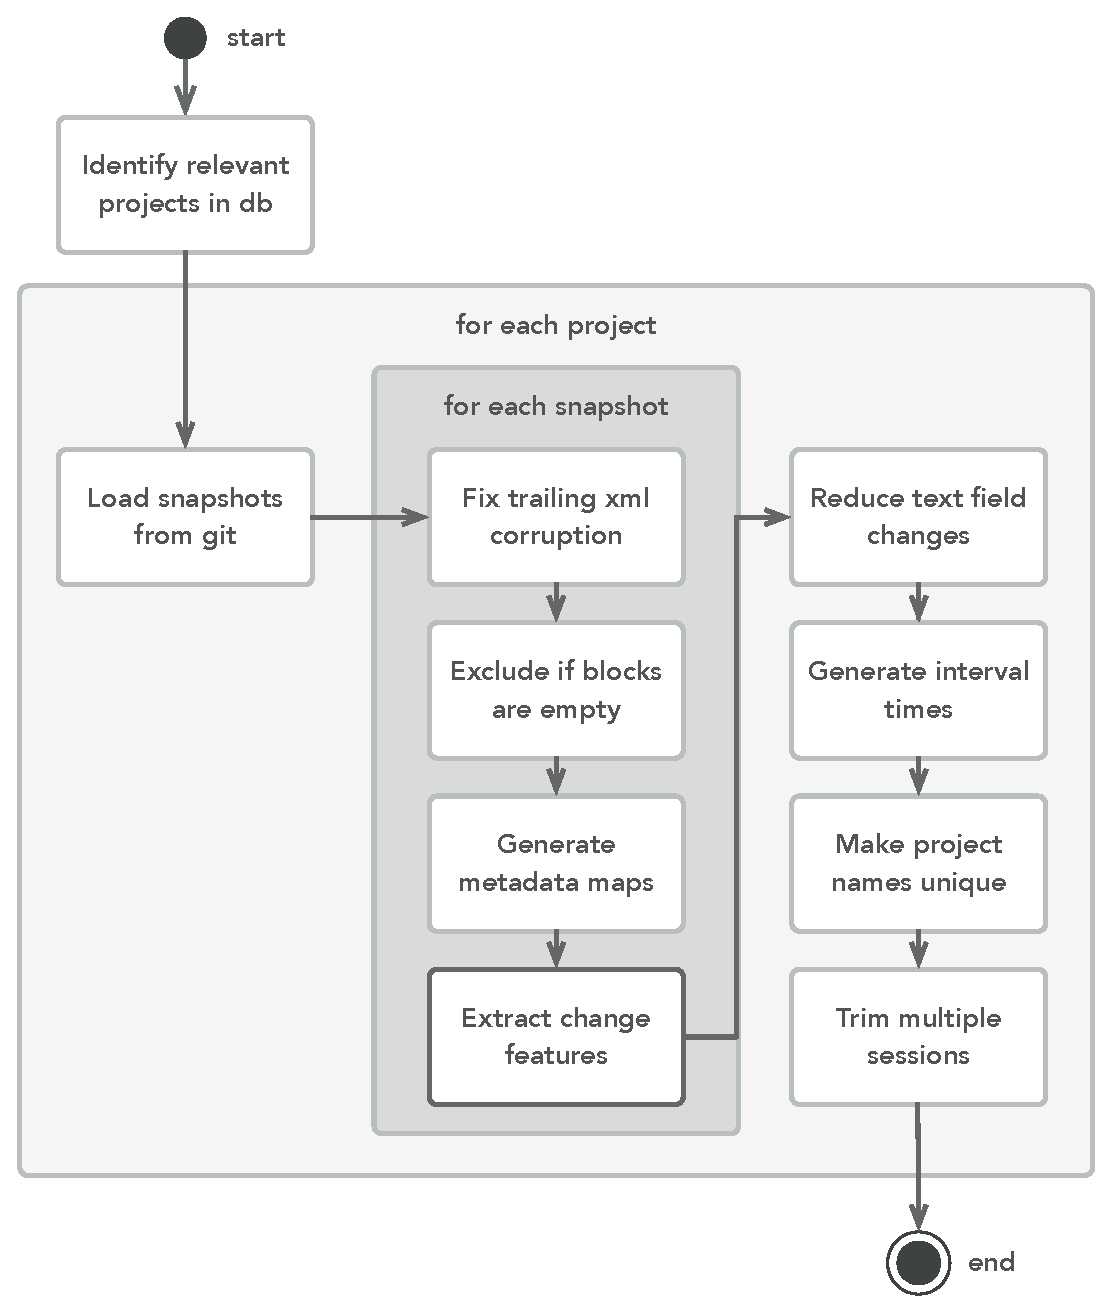
\includegraphics[width=\textwidth]{diagrams/data-import-process}
  \caption[The Data Importing Process]{The data importing process. The entire database was scanned for projects that contain an identifiable element, which were then loaded directly from git. Each change from git was processed for error mitigation and necessary metadata generation, then the features were extracted. After feature extraction, character-wise text field changes were reduced, and then the interval times between snapshots were generated.}
  \label{fig:data-import-process}
\end{figure}

The import pipeline had many tasks to accomplish, starting with identifying the projects that were relevant for analysis. The App Inventor instance that was used for this study was also used for the entirety of the summer camp curricula, so there were many projects captured in the snapshot database that were not part of the activities specific to this study. This was an intentional part of the protocol to make transition easier for the camp students by only having one App Inventor instance with which to interface. The in-class activities were better isolated, so researchers were able to prepare the room in advance to steer the students transparently towards the specialized instance. 

The activities that were part of this study needed to be found in the database. Students had the ability to rename projects at any point, so it was possible (albeit unlikely) that a relevant project could be renamed. Therefore the protocol included a unique element in the projects, a ``magic string'' in a hard-to-find property of the project. The debugging activity and temperature activity each had a unique identifier string, and these strings were included in the starter code that all students were given. These unique elements were then detectable by scanning the files in the git database prior to import. There were instances of students changing the names of the projects, which demonstrated the need of the unique identifier. 

Once a list of projects were identified using their unique elements, those projects were loaded from git into the analysis environment. The git interface opened each project's repository, extracted a list of all commits, and then checked out each commit in turn, capturing the contents of the files for each commit. A commit represented a single snapshot, and the terms ``snapshot'' and ``change'' were used interchangeably to describe the contents of the commit after this stage. 

Each snapshot was checked for corruption at time of import. Following that, two metadata maps were generated for each snapshot: a map of block ID numbers, and a map of block parents. These maps allowed the feature extractor to easily access a block by its ID number (which would require a full tree traversal without), and easily look up the parent of any given block. With the maps generated, the feature extractor would then be able to run. 

After feature extraction, the text field events were reduced (described below), and finally, with the snapshot set complete, interval times between snapshots were generated.

Most stages of the import process were additive and non-destructive, so at the conclusion of import each project and snapshot had all of the data available at all previous steps. For instance, the raw block contents were not lost during feature extraction; the list of features were added to the data structure alongside it. 

The following sections delve further into certain components of the import pipeline, and are presented in pipeline order: corruption mitigation, feature extraction, and text field reduction.


\subsection{Corruption Detection and Mitigation}
Some forms of corruption were found in the snapshot data, all concerning the blocks representation. There were four corruption modes, which are explained below, with their respective mitigation strategies.

The first corruption mode was malformed XML files which contained text beyond the closing XML tag. This, of course, crashed the XML parser. Within the debugging activities, only seven snapshots had this malformation, which were corrected by trimming the excess text. It was noteworthy in those cases that the junk excess text was a repetition of the last characters of the file, lends to a hypothesis of the source of the corruption, discussed below.

The second form was rare, where a snapshot had no contents for the blocks file. In the entire collection of debugging activity snapshots ($n = 6890$), only three snapshots had empty blocks. These snapshots were detected during import and were not included in the research data. The overall history of the projects containing these empty shapshots were unaffected. 

Both of these corruptions were indicative of a bug in the extraction of the block data from blockly in the browser. It was possible that the snapshot mechanism was able to capture the XML file while it was in an inconsistent state, such as mid-write. This bug may be within the Blockly framework itself, and further investigation is recommended before attempting larger-scale deployment of this method.

The two above corruptions were easily mitigated. A third mode of corruption, however, resulted in properly formed XML, but potentially erroneous data. This mode was characterized by multiple changes happening in a single snapshot, which should have been extremely rare, as each snapshot was triggered by an atomic action in the editor. In reality, there was a small amount of caching in the capture mechanism, as discussed in Section \ref{sec:mod-ai}, which may have contributed to this corruption. There was no inherent problem with multiple changes in a single snapshot, if they all occured within the capture window of that snapshot. In these erroneous cases, one or more actions appeared to be inconsistently represented over time, which caused git and the subsequent analysis tools to do, un-do, and re-do the same action in very small spans of time, artificially inflating the representation of those events. 

One project was particularly egregious, and showed this corruption in 71 of its 245 commits, rendering nearly a third of its data unreliable. That project was removed, which left only 50 such potential errors in the remainder of the database, many of which were mitigated by text field accumulator, described in Section \ref{sec:text-acc}. 

A data consistency bug was found where a project was opened over more than one session. In App Inventor, if a project was opened in a second, disjoint session, such as the following day, the block ID numbers change, causing the feature extractors to falsely over-report blocks being deleted and added, when really the same blocks have been re-numbered. The strategy employed was to ignore snapshots that occurred at a timestamp beyond the maximum time of the activity.

The total percentage of potentially erroneous snapshots in the debugging activity dataset was 0.84\%. These are summarized in Table \ref{tab:data-corruption}.

% % Debug:		empty blocks - 3 (now, many were hand-fixed, notes may indicate more)
% %				junk past tag - 7 (now, many were hand-fixed, notes may indicate more)
% %			6890 snapshots total
% % Temperature:	empty blocks - 1 
% %				junk past tag - 4 
% %			2296 snapshots total
	
\begin{table}
\begin{centering}
	\begin{tabular}{l r l p{5.4cm}}
	Corruption Mode 		& \multicolumn{2}{l}{Instance Count} 		& Mitigation Strategy 			\\ \hline
	Empty block file 						&  3 &(0.04\%) 				& snapshot deleted 						\\
	Junk beyond \mintinline{xml}|</xml>| 	&  7 &(0.1\%) 				& junk trimmed, snapshot kept 			\\
	Multiple changes 						& 50 &(0.7\%) 				& accepted as insignificant 			\\
	Multi-session 							&  3 &(0.04\%) 				& data past 40 minutes ignored
	\end{tabular}
	\caption[Data corruption modes]{Data corruption modes, their prevalence, and mitigation strategy.}
	\label{tab:data-corruption}
\end{centering}
\end{table}


\subsection{Feature Extractor}
\label{sec:feature-extraction}

\begin{table}
\begin{labeling}{Blocks Moved in Context}

	\item [Blocks Added] Block(s) were added to the workspace. Nearly always a single block.
	\item [Blocks Deleted] Block(s) were removed from the workspace.
	\item [Blocks Moved in Space] Block(s) moved position on the workspace, but did not necessarily change programmatic meaning.
	\item [Blocks Moved in Context] Block(s) changed programmatic position, indicating a new parent block and a different place in the app's control flow.
	\item [Fields Changed] A block's text field changed. Could be a text literal, a variable or procedure name, or a number literal.
	\item [Properties Modified] One or more properties of a block has changed, which could indicate use of the mutator to change a block's semantics (such as changing the number of addends in an addition block). Intended as a catch-all if the other tests missed something, and was rarely found in the data.
	
\end{labeling}
\caption[Features extracted from snapshots]{Features extracted from snapshot data.}
\label{tab:features-extracted}
\end{table}

The features extracted by this module were listed and described above in Figure \ref{tab:features-extracted}. This section outlines the specific definitions that constitute the feature tests. All of these tests operated on snapshots of the same project that were adjacent in time. They detected differences between the two, often utilizing the metadata maps described above in Section \ref{sec:data-processing}. Source code for these algorithms are presented in Appendix \ref{src:feature-extraction-tests}.

The test for \emph{Blocks Added} and \emph{Blocks Deleted} were the same routine, which assembled a list of blocks by their ID numbers for both snapshots and compared differences between those lists using set arithmetic. 

The test for \emph{Blocks Moved in Space} assembled a list of blocks that were present in both snapshots, and iterated that list looking for blocks who were both top-level and whose coordinates changed. There was an important distinction made here- blocks that were nested within other blocks were not top-level and therefore did not trigger the \emph{Blocks Moved in Space} flag when they moved as a consequence of their parent moving. Only blocks whose parent is the workspace itself may return positive from this test, and then, only if they actually moved on the workspace.

\emph{Blocks Moved in Context} was the opposite of the above test, where it detected if a block moved in computational context, indicated by a changed parent. Similarly, this test assembled a list of blocks common to both snapshots, and iterated across that list. The iteration checked if the parent for the block was the same in both snapshots, and returned true if they were not. 

To detect \emph{Fields Changed}, common blocks were listed and then filtered for field properties. Those fields were searched for cases where the value of the fields differed between the two snapshots.

The final test, \emph{Properties Modified} caught any other modifications to a block. This test was more complex. Like those above, it assembled a list of blocks present in both snapshots. It then ran an exhaustive element-wise equality check on each block, comparing the version in each snapshot. If the equality check returned true, that block did not change in any way. If the equality check was false, then lists of all children for both blocks were assembled, which included properties, data fields, mutator instructions, and other Blockly metadata. This step excluded text fields, as they were covered in a previous test. If the lengths of the lists of children were unequal, then the routine returned true, as these particular blocks definitely changed between the two snapshots. If they have the same number of children, then each pair of children were iterated, and the element-wise equal was applied to each of them, effectively running a first-level recursive equality test. If that test did not find any differences, then the routine returned false. That final false return is a condition that should be impossible, but was included defensively, as there may have been edge cases possible in Blockly that were not common in known to the researchers at the time of this design.


\subsection{Text Field Change Accumulator}
\label{sec:text-acc}
In the course of working on their activities, students often manipulated fields of text, including text literals, variable names, procedure names, and parameter names. Examples of blocks utilizing open text fields are shown in Figure \ref{fig:text-fields}. Whenever a text field was modified, the change event was triggered for every character. This was a degree of granularity too fine for meaningful analysis, as character modification events are considered too primitive to be of use \citep{omori2008change}. The snapshot system at runtime could not discern the beginning and end of field editing events, so the change event feature \emph{Fields Changed} from Table \ref{tab:features-extracted} was grossly over-represented. 

To combat this over-representation, sequences of character-wise change events needed to reduced to their final state, which then represented a single change at the same degree of abstraction as the surrounding block manipulations. This reduction was accomplished with an accumulator algorithm, which scanned a project's change history and identified uninterrupted sequences of field modifications to the same field. The algorithm deleted all but the final \emph{Fields Changed} events, leaving only the final state of the modification for further processing. This algorithm had a 10-second timeout, so sequential edits to the same field would be considered different events if there were more than 10 seconds between them. Changes to different field blocks were also considered a new event. This algorithm is shown and further explained in Appendix \ref{src:reduceFieldChanges}.

\begin{figure}
  \centering
      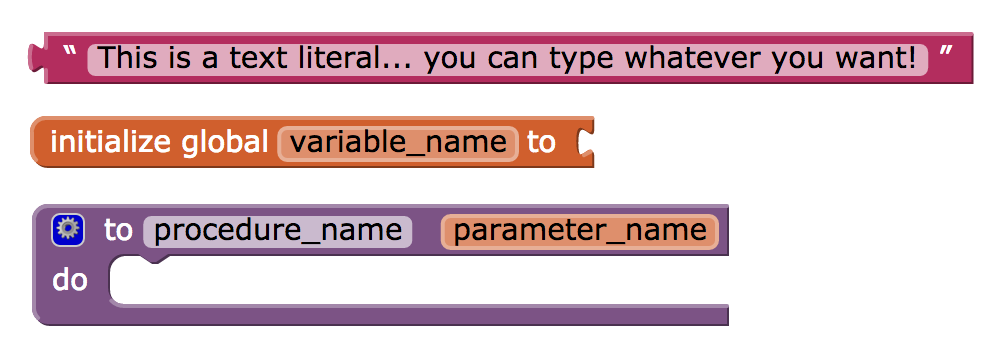
\includegraphics[width=\textwidth]{images/ch4-text-fields}
  \caption[Examples of Text Fields in App Inventor]{Examples of some text fields in App Inventor. All of the fields, represented by the text in shaded bubbles, could be edited arbitrarily by the student.}
  \label{fig:text-fields}
\end{figure}



\section{The Particle Analysis Method}
\label{sec:particle-analysis}

The purpose of this study was to develop a tool, informed by students' fine-grained programming activities, that can aid a teacher in deciding how to apply their resources during a lab session in real time. A significant insight was reached during analysis of the above change-type features, that such a tool could be constrained to standardized, ``on-rails'' programming assignments. These closed-ended assignments constitute the bulk of many curricula in use, such as those described by  \citet{gray2012teaching}, \citet{martin2015dual}, and \citet{morelli2015analyzing}, and are particularly common at the beginning of curricula, when students are still learning the basics. This situation would be the ideal use case for an orchestration aid. 

With this insight, and the constraint it brought, design began for both a visual tool to help a teacher orchestrate, and an analysis method to power it. The resulting method was \emph{particle analysis,} which borrowed its name from the behavior of atoms and molecules. With this method, a solution to an activity can be regarded as a complex molecule, which was built up out of smaller molecules, which were themselves composed of atoms. In this analogy, every individual block was an atom, and were combined on the workspace to make expressions, representing molecules. A solution to an activity was one or more of these molecules, which could have any number of atoms within it. The analogy could be further extended, admittedly weakly, to correspond the solution to an activity with the chemical definition of ``solution,'' a homogeneous mixture composed of two or more substances. 

When you get to the close-enough text analyzer, it calculates Levenshtein edit distance, using an algorithm proposed by \citet{hyyro2001explaining}.


\section{The Classroom Console}
\label{sec:classroom-console}


\chapter{Discussion}
\label{ch:discussion}


\section{Patterns Observed}
\label{sec:patterns}

\begin{figure}
	\centering
	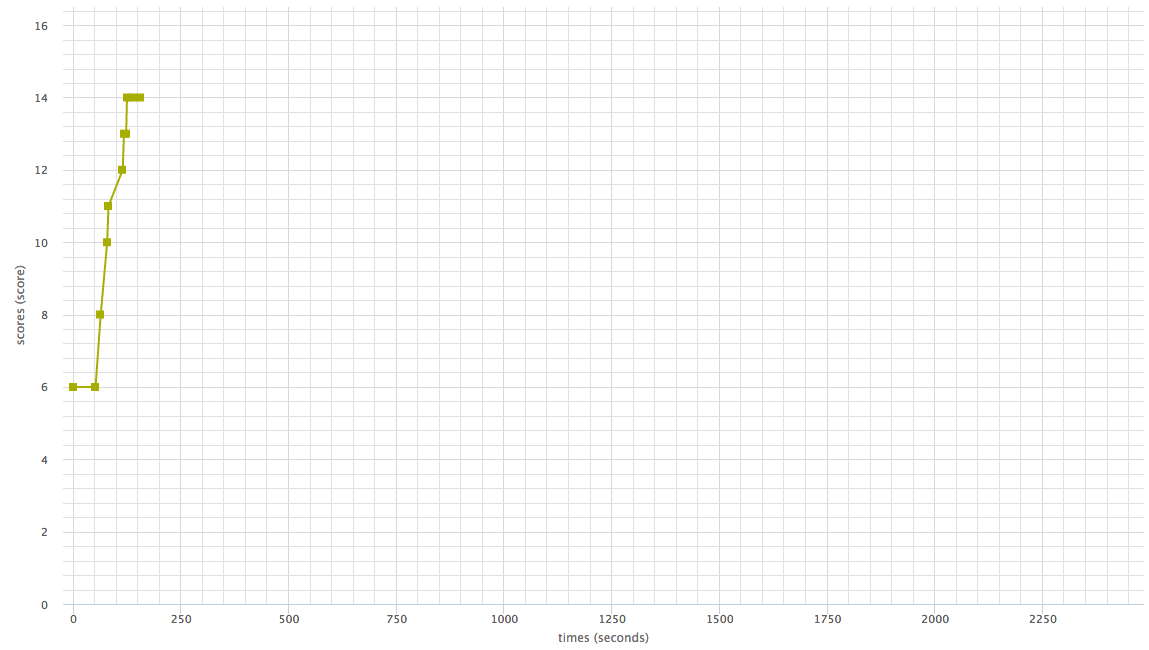
\includegraphics[width=\textwidth]{images/stories/scores-debug-UfaDogfish}
	\caption[Smooth, Rapid Progress of Particle Scores]{Smooth, rapid progress of particle scores, as shown by the student UfaDogfish in the Debugging Activity.}
	\label{fig:smooth_chart}
\end{figure}
Across both activities, three general patterns of particle score progression emerged. The first, called ``smooth'' was a rapid acceleration to the conclusion, where nearly every change improved the score. The ``smooth'' category looks like as if the student already knew the answer, and implemented directly and efficiently. This pattern did allow for slight variation, and smooth-coded projects were not always monotonically increasing, but they were always rapid rises with few changes before the beginning of the upward inflection. An example is shown in Figure \ref{fig:smooth_chart}. Less than a quarter (22\%) of Debugging Activity projects showed this pattern, and just over a quarter (27\%) of the Temperature activity did.

\begin{figure}
	\centering
	\begin{subfigure}{\textwidth}
		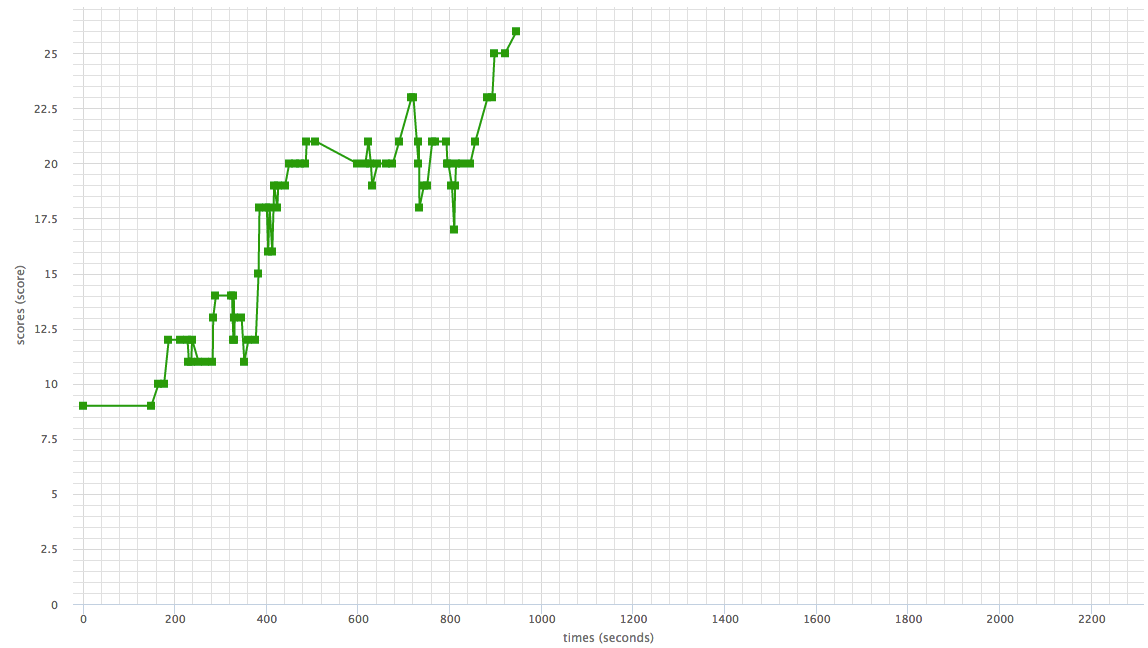
\includegraphics[width=\textwidth]{images/stories/scores-temp-HangzhouTurkey}
		\caption{HangzhouTurkey in the Temperature Activity}
	\end{subfigure}\hfill
	\begin{subfigure}{\textwidth}
		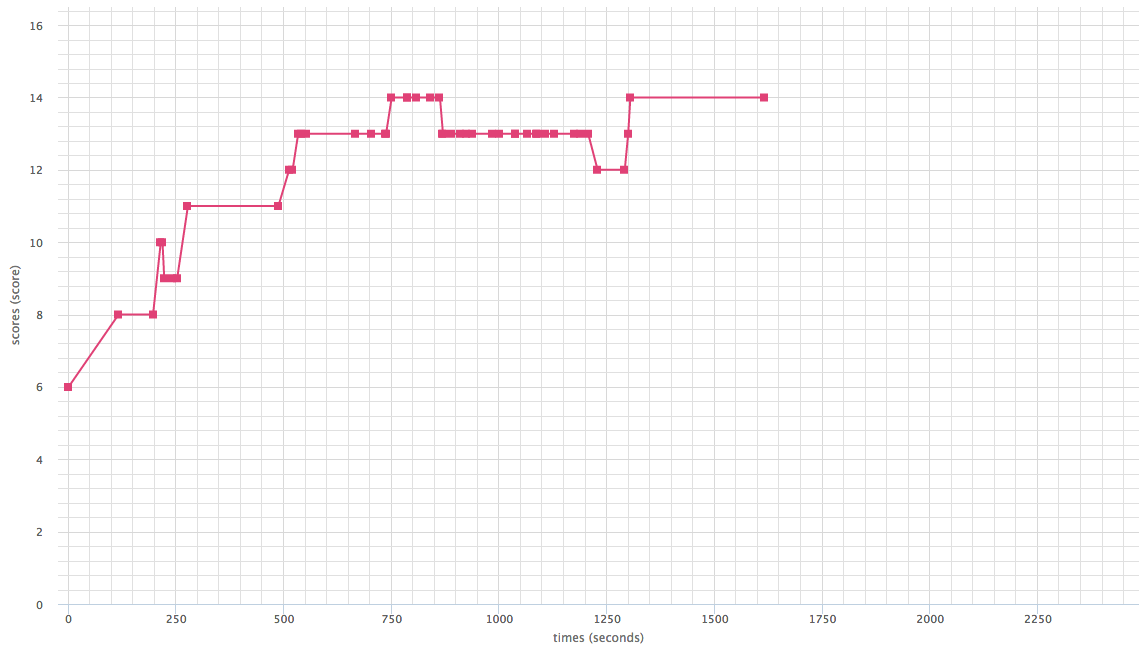
\includegraphics[width=\textwidth]{images/stories/scores-debug-LondonDragonfly}
		\caption{LondonDragonfly in the Debugging Activity}
	\end{subfigure}\hfill
	\caption[``Fits and Starts,'' Typical Progress of Particle Scores]{Two examples of ``Fits and starts,'' demonstrating the typical progress of particle scores.}
	\label{fig:fits_starts_chart}
\end{figure}
The second pattern category was called ``fits and starts'' and represents the most typical trajectory, where the score has periods of progress, non-progress, and sometimes regression, but overall trends upwards and reaches a reasonably successful final state. This was the most broad category, as it was also the one to catch any pattern that was not clearly smooth (above) or flailing (below). Two examples are provided in Figure \ref{fig:fits_starts_chart}, to show the core pattern and some of the allowable variation around it. The Debugging Activity and Temperature Activity projects fell into this category at rates of 49\% and 60\%, respectively. 


\begin{figure}
	\centering
	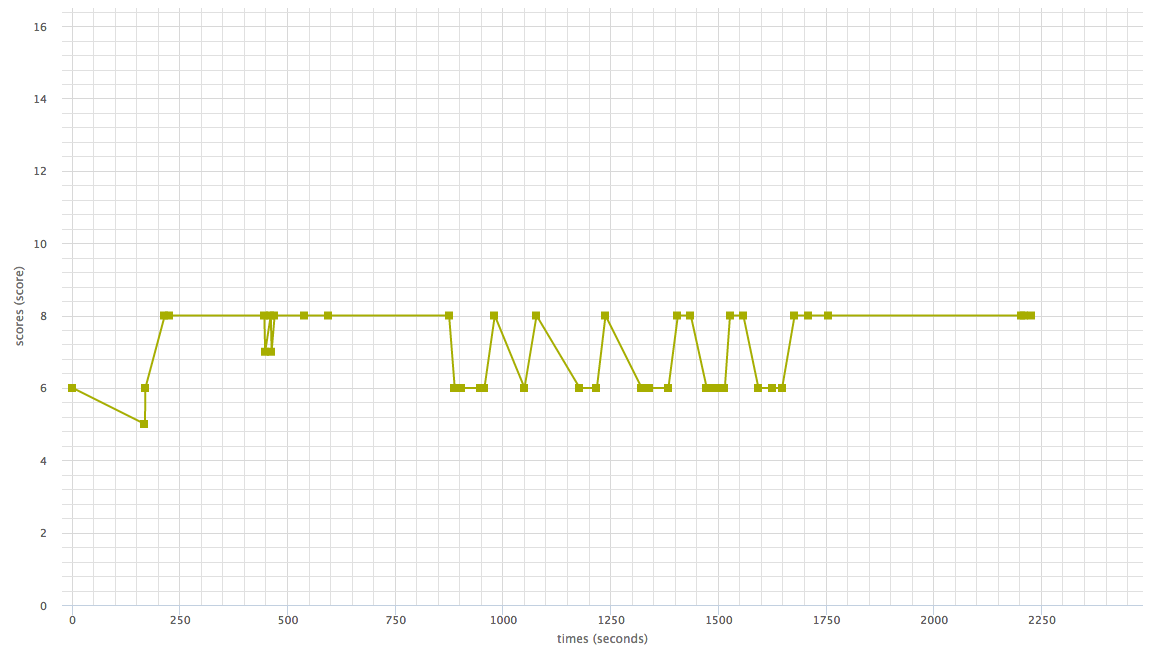
\includegraphics[width=\textwidth]{images/stories/scores-debug-RomePelican}
	\caption[Flailing Pattern, a Lack of Progress of Particle Scores]{Flailing pattern is indicated by a lack of overall progress of particle scores, as shown by the student RomePelican in the Debugging Activity.}
	\label{fig:flailing_chart}
\end{figure}
The third pattern category was ``flailing.'' While the ``fits and starts'' category did allow some flailing behavior, whether score oscillation or non-progress changes, that category always had a generally upwards trend, and resulted in a solution. This category of flailing was reserved for the projects that demonstrated little progress in total, and were entirely flailing behaviors. This pattern is shown in Figure \ref{fig:flailing_chart}. 

A proportion (30\%) of the Debugging Activity projects fell into this category, but, surprisingly, only 13\% of Temperature Activity projects did. We had hypothesized that where the Temperature Activity lacked proper scaffolding there would be more flailing behavior, but the largest category was by far ``fits and starts.'' We can posit that the low rate of apparent flailing at this scale may be due to the aggressive availability of helpers for intervention. The problem may have been sufficiently hard that many students did not even try until they got help from someone. This hypothesis is supported by the wide variation of inflection point, the time where the scores began to increase. Some started right away, while others started nearly at the end of the session period, with many in between. This time translation may be an artifact of the teaching assistants working their way through the classroom, eventually giving everyone the intervention necessary for them to understand and be effective within the problem.

These categories, and the students in each for both activities, is shown in Tables \ref{tab:pattern_names_debug} and \ref{tab:pattern_names_temp}.

\begin{table}
\begin{centering}
	\begin{tabular}{p{\textwidth}}
	\hline \hline
	``Smooth'' (23, 22\%)\\ \hline
		CampoPrairie		
		CiudadWeasel		
		CuiabáGoldfish		
		DetroitShark		
		DortmundBat			
		GorakhpurYak		
		GuayaquilRook		
		HamamatsuFrog		
		JohorGuineaPig		
		KermanshahCockroach1
		LagosRook			
		LibrevilleCrow		
		MendozaAnteater		
		ParisAlligator1		
		PeshawarGnat		
		RangoonBear			
		SantaGrasshopper	
		SeoulOkapi			
		TrujilloLouse		
		TurinFly			
		UfaDogfish			
		VisakhapatnamSheep	
		ZaporizhzhyaFalcon	\\ \hline \hline

	``Fits and Starts'' (51, 49\%)\\ \hline
		AcapulcoDeer		
		CairoCat			
		ChelyabinskSpider	
		ConakryBear		
		CórdobaSalmon	
		DatongPigeon		
		DenverDolphin		
		DhakaClam			
		DhakaEchidna		
		DublinBee			
		FukuokaGoldfinch	
		GuayaquilRook1	
		HangzhouTurkey	
		HangzhouTurkey1	
		HefeiKudu			
		HermosilloSandpiper
		HubliMarten		
		IndoreDogfish		
		IndoreWallaby		
		JinzhouGorilla	
		KaohsiungViper	
		KitakyushuSeal	
		KobeCaterpillar	
		KobeSalamander		
		KuchingCheetah		
		LahoreLapwing		
		LondonDragonfly		
		LusakaOx			
		MoreliaOx			
		MultanFrog			
		MunichTermite		
		NanchangOwl			
		OnitshaWombat
		PermHerring
		PhoenixWeasel
		PointeCheetah
		PueblaVulture
		SeoulSheep
		ShahChinchilla
		SholapurSandpiper
		SurabayaChimpanzee
		TaichungRook
		TaizhouSwallow
		TbilisiKudu
		TijuanaOctopus
		VladivostokCurlew
		WarangalStinkbug
		WroclawRat
		XianAntelope
		YanchengGoose
		ZhangjiakouSardine		\\ \hline \hline
	``Flailing'' (31, 30\%)\\ \hline
		CalgaryHyena
		ChongjuOwl
		HachiojiPeafowl
		HamadanMouse
		HaoraDragonfly
		KadunaAlpaca
		KermanshahCockroach
		KhabarovskBoar
		MakhachkalaWasp
		MultanVulture
		NagpurAlpaca
		NiyalaAlligator
		OkayamaMarten
		OklahomaGiant
		ParisAlligator
		PhiladelphiaWoodpecker
		QuerétaroMule
		QuitoShark
		RomePelican
		SapporoWoodcock
		SarajevoDuck
		SurabayaTermite
		SuwonGoldfish
		TaiyuanDinosaur
		TianjinAlbatross
		TripoliSandpiper
		ValenciaFox
		VijayawadaOtter
		WarsawCrocodile
		XuzhouLoris
		YaroslavlCattle	\\ \hline

	\end{tabular}
	\caption[Categories of Progress Patterns for the Debugging Activity and the Students in them]{Categories of Progress Patterns for the Debugging Activity and the Students in them.}
	\label{tab:pattern_names_debug}
\end{centering}
\end{table}

\begin{table}
\begin{centering}
	\begin{tabular}{p{\textwidth}}
	\hline \hline
	``Smooth'' (8, 27\%)\\ \hline
		DortmundBat
		HubliMarten
		KermanshahCockroach
		MendozaAnteater
		RangoonBear
		TbilisiKudu
		UfaDogfish
		ZaporizhzhyaFalcon
		\\ \hline \hline
	``Fits and Starts'' (18, 60\%)\\ \hline
		DatongPigeon
		FukuokaGoldfinch
		HangzhouTurkey
		KobeSalamander
		LondonDragonfly
		PhoenixWeasel
		PointeCheetah
		PueblaVulture
		QuerétaroMule
		ShiheziBat
		SurabayaChimpanzee
		SurabayaTermite1
		TaiyuanDinosaur
		TaizhouSwallow
		VeracruzDotterel
		VisakhapatnamSheep1
		VladivostokCurlew
		WroclawRat
		\\ \hline \hline
	``Flailing'' (4, 13\%)\\ \hline
		Rostov-na-DonuLapwing
		Rostov-na-DonuLapwing1
		SurabayaTermite
		VaranasiOstrich
		\\ \hline

	\end{tabular}
	\caption[Categories of Progress Patterns for the Temperature Activity and the Students in them]{Categories of Progress Patterns for the Temperature Activity and the Students in them.}
	\label{tab:pattern_names_temp}
\end{centering}
\end{table}



\section{Detailed Case Analysis}
\label{sec:case_analysis}
A selection of student projects were chosen for case analysis, presented here. They were selected to represent the good, the bad, and the interesting. For each, a chart is provided that shows their score in the activity over time. These charts are drawn to the same scale within an activity to allow them to be visually comparable. Additionally, some samples from the code playback history are included, which represent highlights of the student's actual code states to provide concrete explanation for the particle scores.

\subsection{The Good: CampoPrairie}
\begin{figure}
	\centering
	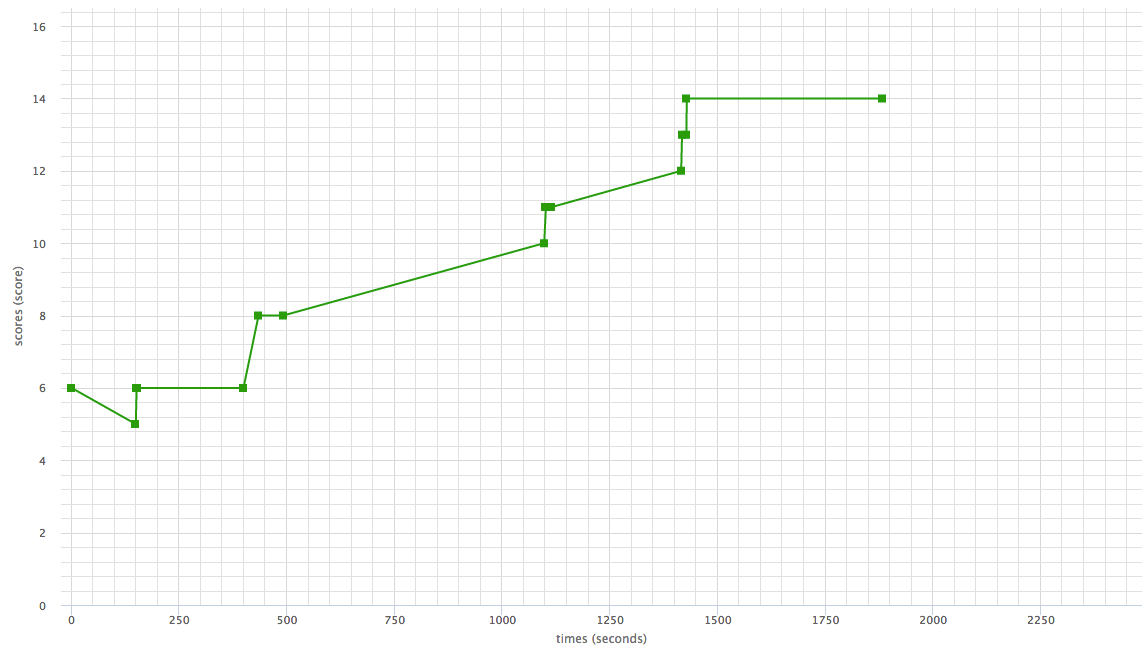
\includegraphics[width=\textwidth]{images/stories/scores-debug-CampoPrairie}
	\caption[Good: CampoPrairie Debugging Activity Particle Scores]{Good: CampoPrairie Debugging Activity Particle Scores.}
	\label{fig:CampoPrairie_chart}
\end{figure}

\begin{figure}
	\centering
	\begin{subfigure}{.45\textwidth}
		\fbox{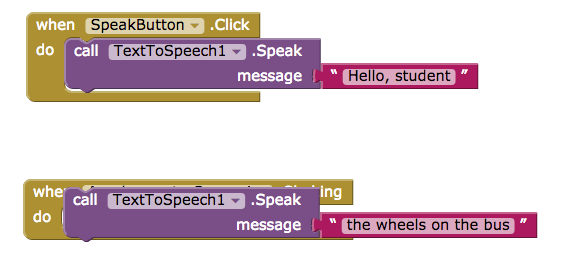
\includegraphics[width=\textwidth]{images/stories/blocks-debug-CampoPrairie/1}}
		\caption{2:29 block accidentally knocked out of place} 
	\end{subfigure}\hfill
	\begin{subfigure}{.4\textwidth}
		\fbox{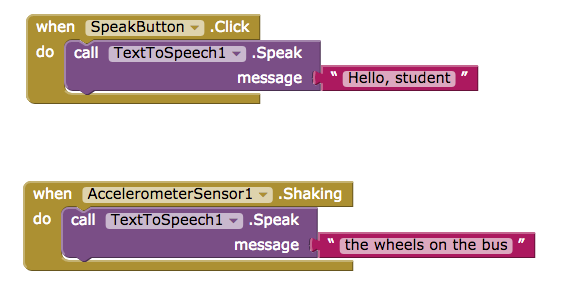
\includegraphics[width=\textwidth]{images/stories/blocks-debug-CampoPrairie/2}}
		\caption{2:31 block knocked back in} 
	\end{subfigure}
	\begin{subfigure}{.45\textwidth}
		\fbox{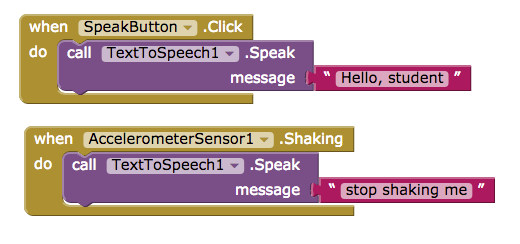
\includegraphics[width=\textwidth]{images/stories/blocks-debug-CampoPrairie/3}}
		\caption{7:14 first bug solved} 
	\end{subfigure}\hfill
	\begin{subfigure}{.45\textwidth}
		\fbox{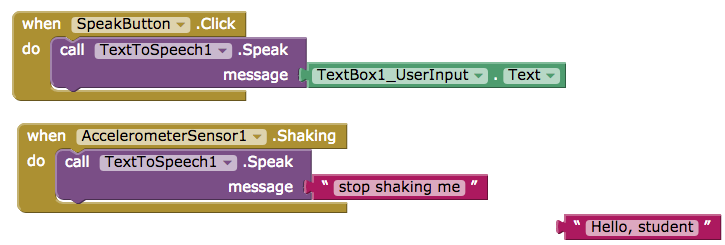
\includegraphics[width=\textwidth]{images/stories/blocks-debug-CampoPrairie/4}}
		\caption{18:21 second bug solved} 
	\end{subfigure}\hfill
	\begin{subfigure}{.45\textwidth}
		\fbox{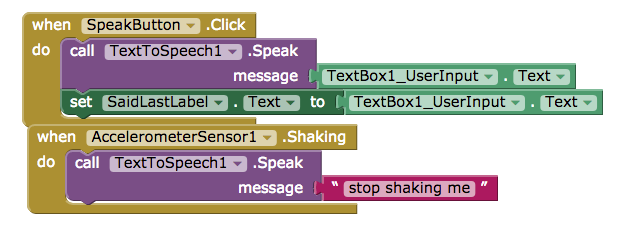
\includegraphics[width=\textwidth]{images/stories/blocks-debug-CampoPrairie/5}}
		\caption{23:48 final bug solved} 
	\end{subfigure}

	\caption[Good: CampoPrairie Debugging Activity Blocks Samples]{Good: CampoPrairie Debugging Activity Blocks Samples. This student completed the activity with minimal difficulty.}
	\label{fig:CampoPrairie_blocks}
\end{figure}

From the Debugging Activity, the assessor looking at blocks playback declared this student ``knew exactly what to do,'' and was coded as ``great'' efficacy. However, this student did not attempt the most difficult subgoal. This student is representative of the typical successful path for this activity. The observation that they quickly ascertained, or already knew, the strategy is supported by the score chart in Figure \ref{fig:CampoPrairie_chart}, which shows a quick and nearly monotonic progression towards the final state. This student reached the solution state in just under 24 minutes.

The brief regression at the beginning of their path is a common and trivial mistake, where a valid block was momentarily knocked out of its parent block, and then quickly re-inserted. This can be seen in the block playback samples in Figure \ref{fig:CampoPrairie_blocks}.


\subsection{The Bad: YaroslavlCattle}
\begin{figure}
	\centering
	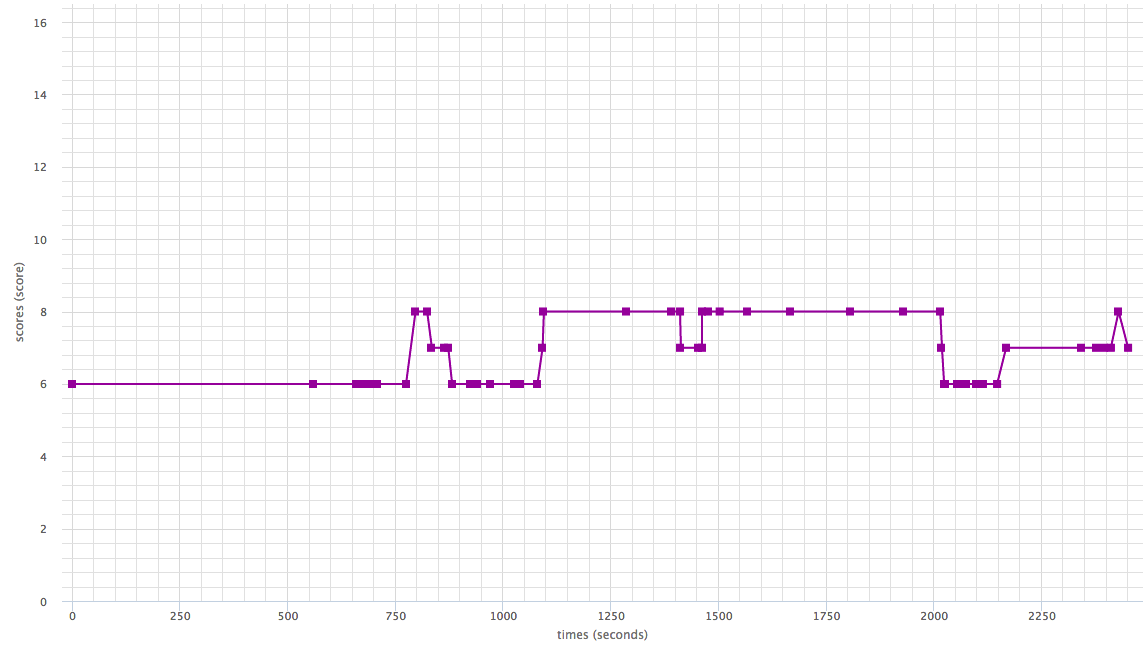
\includegraphics[width=\textwidth]{images/stories/scores-debug-YaroslavlCattle}
	\caption[Bad: YaroslavlCattle Debugging Activity Particle Scores]{Bad: YaroslavlCattle Debugging Activity Particle Scores. This student never progressed more than trivially, despite trying for over 30 minutes.}
	\label{fig:YaroslavlCattle_chart}
\end{figure}

\begin{figure}
	\centering
	\begin{subfigure}{.45\textwidth}
		\fbox{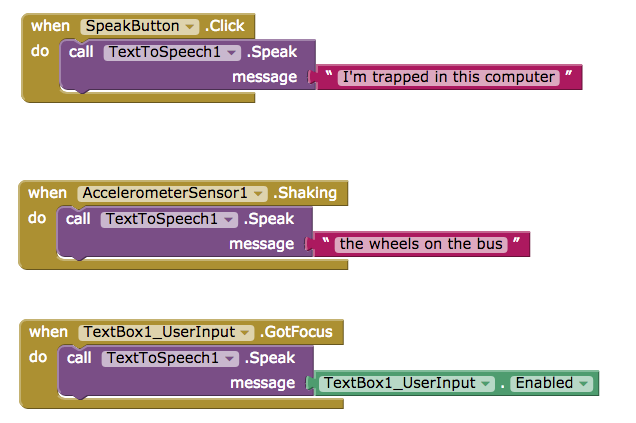
\includegraphics[width=\textwidth]{images/stories/blocks-debug-YaroslavlCattle/1}}
		\caption{11:31 introduced irrelevant \emph{GotFocus} event handler, and populated it with an irrelevant property getter.}
	\end{subfigure}\hfill
	\begin{subfigure}{.4\textwidth}
		\fbox{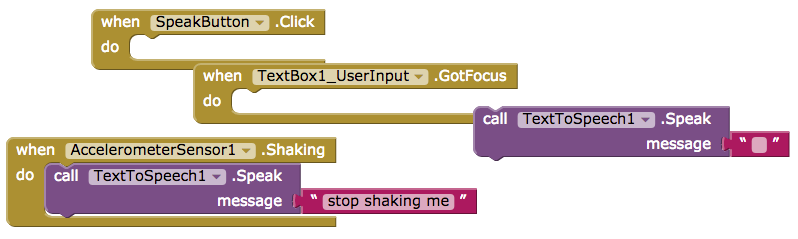
\includegraphics[width=\textwidth]{images/stories/blocks-debug-YaroslavlCattle/2}}
		\caption{14:24 after deleting it, re-introduced the same event handler.} 
	\end{subfigure}
	\begin{subfigure}{.45\textwidth}
		\fbox{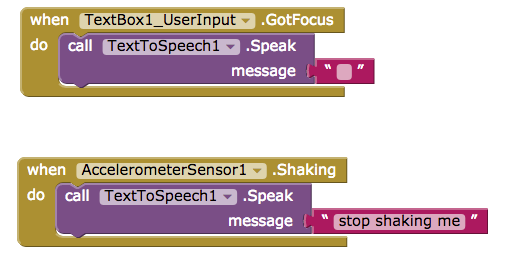
\includegraphics[width=\textwidth]{images/stories/blocks-debug-YaroslavlCattle/3}}
		\caption{16:10 effectively back at the start, a state revisited many times.} 
	\end{subfigure}\hfill
	\begin{subfigure}{.45\textwidth}
		\fbox{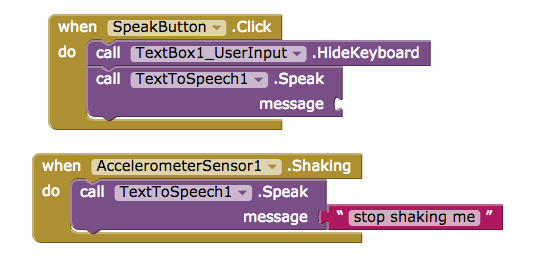
\includegraphics[width=\textwidth]{images/stories/blocks-debug-YaroslavlCattle/4}}
		\caption{23:31 introduced irrelevant \emph{HideKeyboard} block} 
	\end{subfigure}\hfill
	\begin{subfigure}{.45\textwidth}
		\fbox{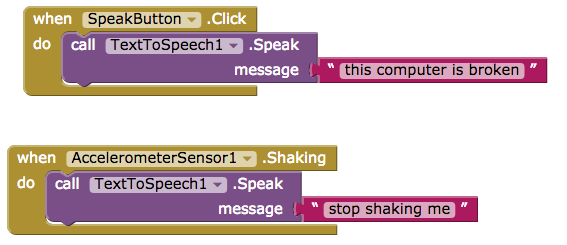
\includegraphics[width=\textwidth]{images/stories/blocks-debug-YaroslavlCattle/5}}
		\caption{26:07 non-topical text entry} 
	\end{subfigure}\hfill
	\begin{subfigure}{.45\textwidth}
		\fbox{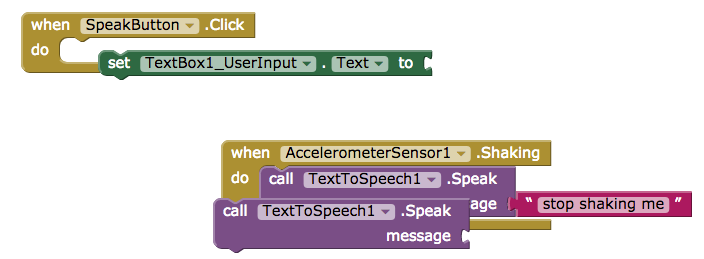
\includegraphics[width=\textwidth]{images/stories/blocks-debug-YaroslavlCattle/6}}
		\caption{40:51 final, inconsistent state} 
	\end{subfigure}

	\caption[Bad: YaroslavlCattle Debugging Activity Blocks Samples]{Bad: YaroslavlCattle Debugging Activity Blocks Samples. This student flailed considerably and made only minor progress.}
	\label{fig:YaroslavlCattle_blocks}
\end{figure}
This student flailed heavily in the Debugging Activity, and appeared to lack traction in understanding the problem. From viewing the blocks playback (Figure \ref{fig:YaroslavlCattle_blocks}), this student repeatedly attempted to construct the same incorrect blocks assembly. They also wrote off-topic prose into text literals, including, at one point, the entirety of the poem ``Twinkle Twinkle Little Star,'' and later, the theme song from the Mickey Mouse Club. This behavior of off-topic text was observed occasionally, and we posit that it is an indicator of lack of traction in the problem. This may be a detectable feature suitable for the teacher's classroom console. An intervention from a teacher or assistant was likely necessary for this student, who never accomplished more than the simplest subgoal. 


\subsection{Interesting: WarangalStinkbug}
\begin{figure}
	\centering
	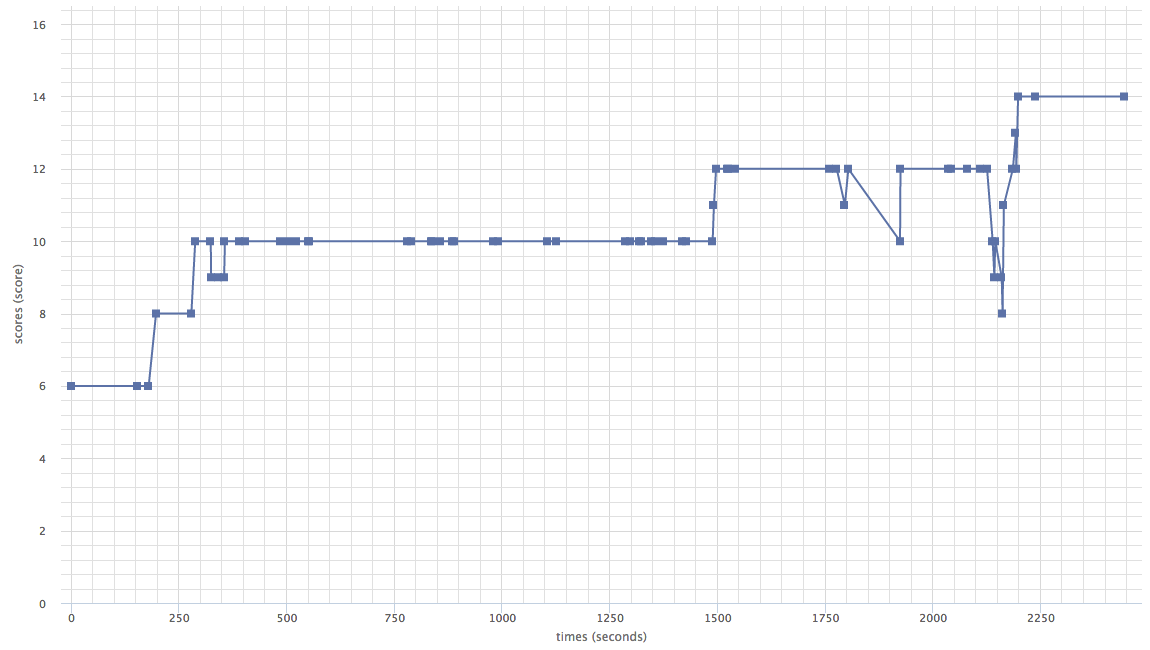
\includegraphics[width=\textwidth]{images/stories/scores-debug-WarangalStinkbug}
	\caption[Bad: YaroslavlCattle Debugging Activity Particle Scores]{Bad: YaroslavlCattle Debugging Activity Particle Scores. This student flailed initially, then was later successful.}
	\label{fig:WarangalStinkbug_chart}
\end{figure}
In the Debugging Activity, a student was observed via playback assessment with ``some flailing in the beginning'' and later success. This was coded as both ``flailing'' and ``good efficacy,'' and that duality makes for a compelling case to analyze. This student started off well at the very beginning, and quickly solved the first bug, and the achieved the simple version of the second bug's solution. After that, this student was unable to make progress for over 20 minutes, during which time they added and deleted a variety of unrelated blocks in turn. This student eventually started making incremental progress. The quick drops in score, followed by immediate return, were caused by a set of blocks that were momentarily removed from their proper context, and then re-inserted. This behavior is common, so large drops in score that are short in duration are not interesting features.


\subsection{Interesting: DenverDolphin \& YanchengGoose}
\begin{figure}
	\centering
	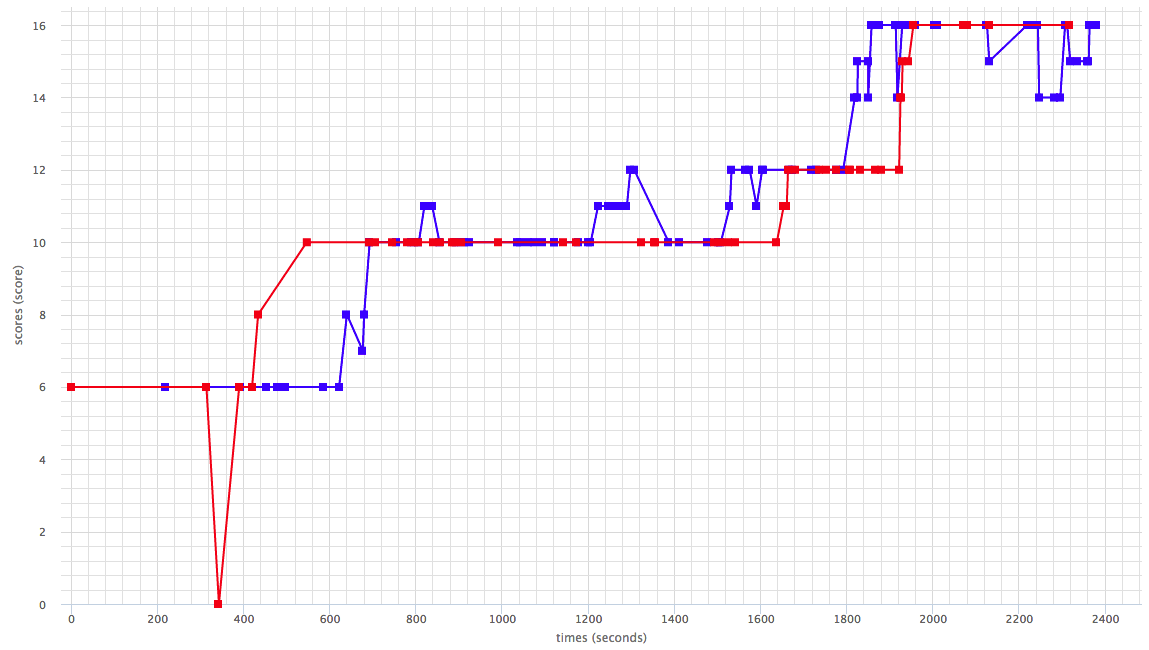
\includegraphics[width=\textwidth]{images/stories/scores-debug-dolphin-goose}
	\caption[DenverDolphin \& YanchengGoose Debugging Activity Particle Scores]{DenverDolphin (blue) \& YanchengGoose (red) Debugging Activity Particle Scores. These were the only students to solve or nearly solve the final subgoal of the activity.}
	\label{fig:dolphin_goose_chart}
\end{figure}
\begin{figure}
	\centering
	\begin{subfigure}{.45\textwidth}
		\fbox{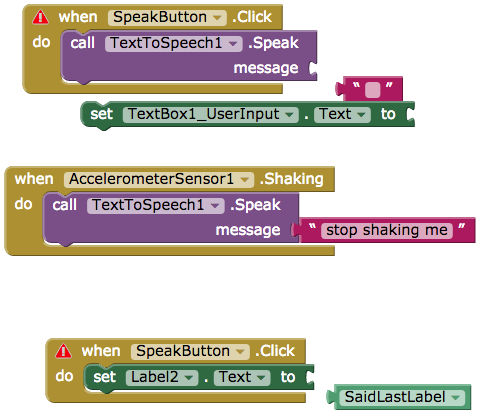
\includegraphics[width=\textwidth]{images/stories/blocks-debug-DenverDolphin/1}}
		\caption{25:04} %frame 130
	\end{subfigure}\hfill
	\begin{subfigure}{.4\textwidth}
		\fbox{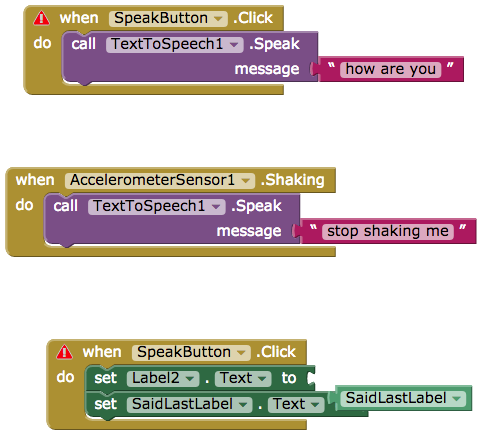
\includegraphics[width=\textwidth]{images/stories/blocks-debug-DenverDolphin/2}}
		\caption{26:08} %frame 142
	\end{subfigure}
	\begin{subfigure}{.45\textwidth}
		\fbox{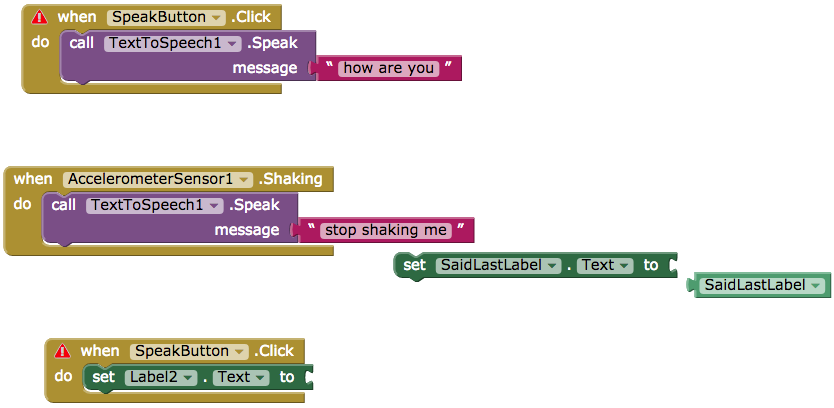
\includegraphics[width=\textwidth]{images/stories/blocks-debug-DenverDolphin/3}}
		\caption{26:43} %frame 159
	\end{subfigure}\hfill
	\begin{subfigure}{.45\textwidth}
		\fbox{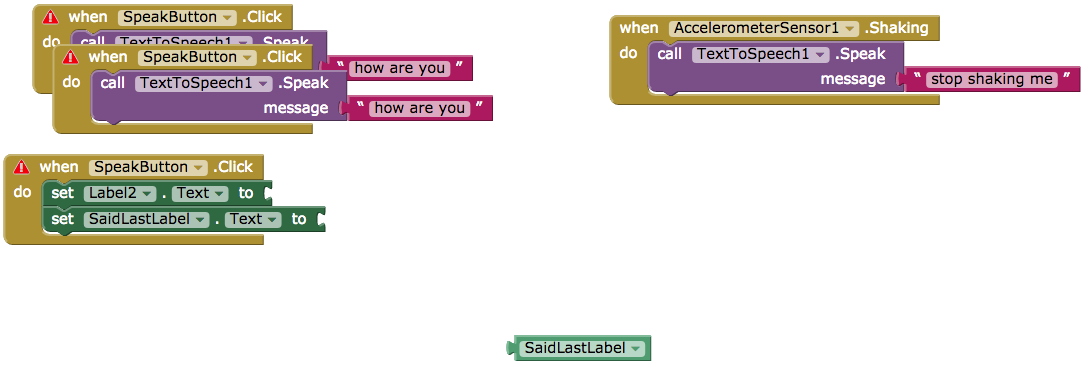
\includegraphics[width=\textwidth]{images/stories/blocks-debug-DenverDolphin/4}}
		\caption{29:36} %frame 181
	\end{subfigure}\hfill
	\begin{subfigure}{.45\textwidth}
		\fbox{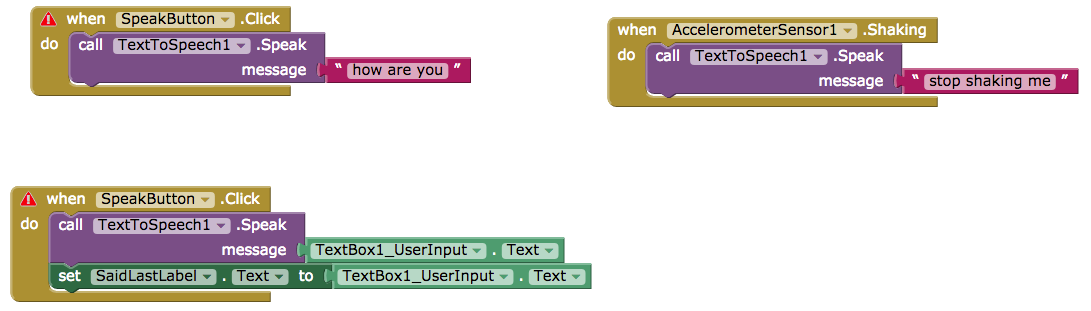
\includegraphics[width=\textwidth]{images/stories/blocks-debug-DenverDolphin/5}}
		\caption{32:21} %frame 217
	\end{subfigure}\hfill
	\begin{subfigure}{.45\textwidth}
		\fbox{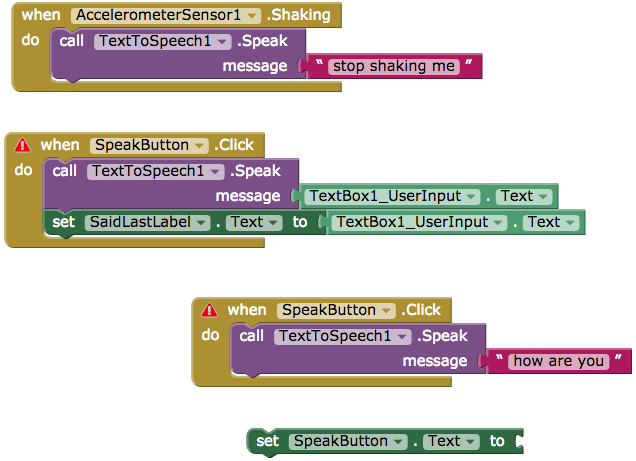
\includegraphics[width=\textwidth]{images/stories/blocks-debug-DenverDolphin/6}}
		\caption{39:46 and final state}
	\end{subfigure}

	\caption[DenverDolphin Debugging Activity Blocks Samples]{DenverDolphin Debugging Activity Blocks Samples, showing the final 15 minutes of work. This student neglected to delete duplicate \emph{SpeakButton.click} handler, but otherwise had the entire activity solved.}
	\label{fig:dolphin_blocks}
\end{figure}

Two students nearly completed the entire Debugging Activity, but had an artificially high particle score, demonstrating a current weakness in the implementation of the particle analysis technique. 

Student DenverDolphin was coded as from blocks playback with ``extreme flailing,'' and judging from Figure \ref{fig:dolphin_goose_chart}, that assessment was correct. This student experienced long periods of activity with no forward progress, and many points of momentary progress followed by regression. YanchengGoose was similar, with a completely flat period of activity from 546 to 1637 seconds, a period of over 18 minutes with no forward progress. Both of these students, however, appeared to slowly worked their way up to the common solution as they approached thirty minutes, and then quickly found their way to an even higher particle score. The students definitely exhibited flailing behavior, but their non-productive behavior did eventually give way to a solution. However, an additional misunderstanding caused both students to access a weakness in the current particle analysis implementation, creating an artificially high score while not solving the final problem.

Upon inspection of the blocks playback, DenverDolphin never actually solved the final bug completely, though came incredibly close. They experimented over a period of about 10 minutes, slowly bringing out more of the relevant blocks, and then constructed the entirely correct event handler and actions. Sadly, they never deleted the old event handler that the new one superseded. App Inventor requires each event handler be unique, and when it encounters duplicates, both are labeled with an error indicator and both are ignored. This student was one small realization away from completing the bug they labored against. A sampling of this student's activity in the final 15 minutes of their session can be seen in Figure \ref{fig:dolphin_blocks}. YanchengGoose exhibited the same behavior, was caught on the same stumbling block, and triggered the same score-inflation weakness. 

As there are three subgoal in the Debugging Activity, there are three separate goal tests, whose scores are summed. If all were executed at the same time, the maximum score would be 16. But that would be impossible with working solutions, as solutions to successive goals actually supersede previous ones, deprecating older code structures. With that, a perfect solution is actually a score of 14. A score of 16 demonstrates a current weakness with the analysis, that a solution can still be over-represented, artificially inflating the score by a small amount.



\section{Evaluating the Classroom Console}
\label{sec:console_evaluation}

% assert console is good, using:
%	Teacher "focus group" feedback
%	Comparison against design goals from literature - Dillenbourg
The researchers recruited a small group of instructors who use App Inventor in their classrooms to see, discuss, and evaluate the Classroom Console. They were interviewed individually, where they were shown the some brief background, the particle assessment concept, a demonstration of the Console. Their reactions were overwhelmingly positive, where the most common question was a form of ``when can I use this?'' The instructors also provided criticism, identified potential weaknesses in the design, and engaged in discussion on how to overcome those weaknesses. One instructor, during the demonstration said, ``I can see right now two students I want to go talk to.'' These discourse are summarized below.

The focus group instructors had two middle school teachers, two middle and high school specialty teachers, two high school and undergraduate instructors, and one undergraduate professor in charge of five lab sections. Their localities included the United States east coast and Midwest, and South America. 

Concerns raised by teachers: 
\begin{itemize}
\item Easily identifies ``needy'' students, who ask for help immediately without first trying on their own. %TODO there is definitely a term for this
\item Similarly, this tool makes it easy to identify high-performing students who can be tasked to help their struggling peers. (Researchers did not realize the tool could be used to identify exemplary performance just as easily as flailing.) 
\item The above matching feature could be automated, in the style of \citet{Diana:2017:IDR:3027385.3027441}.
\item Sometimes you only see students every 8-9 school days, so catching idle periods of mere minutes can be critical. 
\item It is possible for a student who is disengaged to be sitting next to an engaged student, and they both look like they're engaged.
\item When a student returns from a bathroom break, the tool can help assess how quickly they resume engagement.
\item Greatly aids cases where students don't do anything because they know they can get away with it.
\item Training instructors to use the tool may be non-trivial, especially when requiring them to develop their own activities with it. 
\item As the tool is an inexact proxy, experience with the tool may increase the instructor's efficacy with it.
\item High school students are especially afraid to fail, so they often choose not to try anything. This helps identify that behavior.
\item Student feedback often includes the complaint that they did not get enough attention. They could be feeling frustration that the instructor is not seeing, and this helps the instructor gain access into that.
\end{itemize}

Requested Features
\begin{itemize}
\item An automated flag to visually highlight students who are currently exhibiting significant flailing behavior.
\item Flexibility in timeout bar. Some activities and classrooms will have different time frames that would be considered concerning.
\item Treatment for score regression, which is currently not highlighted. 
\item Take the start point with gift code into consideration, and flag the teacher if the student drops below that point, as they have broken their starting configuration and likely need help restoring it.
\item History so teachers can replay or otherwise visual past classroom sessions, and compare them over time. Line chart of the session.
\item Reporting to demonstrate a student's progress in labs over time, suitable for program assessment. 
\item Control over layout, so student locations in Console reflect the seating plan of the classroom.
\item Ability to define your own activities and their corresponding solution particles.
\item Pseudo-anonymized student identifiers, such that the console could be displayed on the projector while the teacher moves around the room.
\end{itemize}

One analysis idea presented by an instructor was to display the \emph{number of attempts} at a certain point of a problem, which would allow the teacher to expect and allow a certain number of attempts before requiring intervention. This method would require further work to better define what an ``attempt'' should mean in general context, and in an activity-specific context.

The instructors were overall excited about the tool, and raised real-world concerns that could further inform the design of the Classroom Console. The instructors declared that the design was ready for prototype use, all citing their desire to use it to enhance their teaching practice.


\section{Conclusions}
\label{sec:conclusions}
A ``flailing detector'' to aid teachers in real-time classroom orchestration is possible when the problem is constrained to known activities with predictable solutions. The particle analysis method delivers a lightweight, good-enough metric to deliver this visual aid in real time. In post-hoc analysis, particle analysis data can be visualized differently to ascertain the trajectories experienced by students. In real time and post-hoc, the visualizations of the particle analysis data lend themselves to easy interpretation of student progress within their activities. Post-hoc tools such as those in this study were requested by teachers while evaluating the real-time console. A package of tools to enable real-time assessment and deeper analysis and reporting after the fact is in demand for teachers who use programming exercises (labs) in the classroom. A number of additional features were identified that would further improve the accuracy of the particle analysis method, such as looking for off-topic strings as a sign of lack of problem traction. Many language- and implementation-specific improvements were also identified to improve the method. This method and its tools are not heavily dependent on language-specific features or work flows, and can be ported to work with any Blockly-based language immediately, and can be used to inform particle analysis implementations in other block, visual, and textual language environments.

%\section{Recommendations} 
% \label{sec:recommendations}
% We do not recommend using git as a database. Further recommendations of legitimate scientific and educational merit will be added as part of the full dissertation.


\section{Future Work}
\label{sec:futurework}

As previously mentioned, there is ample future work to be done in understanding the reasoning behind behavior choices, with particular support to mis-attribution of failure and success. Investigation into this mis-attribution should be conducted, to use traditional methods of assessing student mindset combined with the power of fine-grain snapshot analysis. 

The change-type features that were extracted from these data would likely be useful in a study where an independent variable describing a behavior of interest could be collected. Such an experiment could be looking for off-task behavior, comparing expert and novice patterns, studying a particular class of common mistake, or any other pattern. With tightly-controlled observations to record the ground truth of the behavior in question, change-type data such as these could be mined against that ground truth to find corresponding relationships. 

A teacher-ready product using particle analysis would consist of a library of solution particle definitions matching activities from the curriculum. The curriculum for App Inventor is largely stable, if varied, and creating solution particle definitions for the most common assignments would benefit teachers active in many different curriculum programs. 

Adding custom definitions of solution particles to match specific activities would require, in its current form, a researcher or developer to design the particles. However, this is not due to the particles being difficult to imagine, but the degree of complexity of the tools with which the particles are currently defined. The elements that make up particles are already defined, abstracted entities that do not require direct manipulation of the underlying blocks representation. One slight exception is the ``close enough'' text comparator, described in Section \ref{sec:close-enough-text}, which was hard-coded with allowable edit distances. It would require a bit more generalization to meet the other elements. But with some wrapping and smoothing, a small language could be developed to express all possibilities of solution particles in a way that would be more accessible to curriculum developers. An even better tool would be able to capture a solution directly from App Inventor and disassemble it into constituent particles automatically. This tool would be the most accessible, and anyone who knows App Inventor to also define canonical solutions for use in the particle analyzer, and with that, the classroom console. 

\subsection{Classroom Console and Learning Management Systems}
Different kind of research, but there still is possibility some lit-backed research on how to do this effectively. Take a stab with some lit right here.

\subsection{Towards Programming Skill Assessment}
Someday may have an entire curriculum of activities, and data of kids doing these activities over time. Collected in aggregate for research purposes, could start to isolate skills that are exercised by different activities, and begin to understand how those skills are developing over the course of a curriculum.

\subsection{Solution Particles as Indicators for Further Analysis}
The particle analysis method is, at its core, a feature extractor for snapshot data. For every snapshot, it provides an indicator of progress. That measure of progress has potential to be used to advance real-time classroom tools, and to inform future research. 

One example would be to use solution particle scores as an indicator for same-state. If a student returns to an identical or near-identical state of their code, that student may be experiencing some sort of flailing, in the form of a non-productive iterative behavior. Detecting a return to a previous state is certainly possible from snapshot data, but is potentially computationally expensive. The fast particle scores could serve as a beacon, and could be used as a signal to automatically deploy the more expensive same-state algorithm. The solution scores could reduce the set of possible comparisons for a given snapshot state dramatically, likely allowing it be performed in real-time. This measure could be added to the classroom console or other teacher analytic tool to add richness to the teacher's view of the students' behavior. 
%TODO find some lit references about same-state detection in programming?

The particle score could also be used as a variable for future experiments, and could help to uncover patterns of other properties that correspond with progress made, stalled, or regressed. One such study could take the scores over time in post-hoc data, and encode periods of those histories into states abstract states, describing patterns in the scores, such as flat changes (active non-improvement), fast progress, and regression. These states could be used in in a machine learning experiment to extract correlating patterns in other data, similar to \citet{tissenbaummodeling}, hopefully revealing properties that may be related to those behaviors.

One such design could use a Hidden Markov Model to determine the threshold for automatic flailing detection. This auto-detection could then flag students above threshold in the Classroom Console, further aiding the teacher in deciding where to direct their resources. Inputs to this method would be the particle score graph, or segments of it, with specific measures extracted: interval since last frame, score increase, score decrease, or score the same. 

Further investigation should be given to conditions where students ``win'' at flailing--- when a non-advancing set of changes yields and does not yield advancement. This may be possible with the data from this study. Hypotheses include that flailing/play periods will be different per assignment, and there may be a method, such as the one in the above paragraph, to determine what is reasonable for a particular assignment. 

It may also be possible to use instrumentation to detect the spread of code artifacts through a classroom, which could be indicative of integrity, or simply teach us how concepts propagate through a student population. Just looking at code playback, there are projects that intuitively ``look like'' they might be engaged in copying solutions. This intuition is based on sudden appearance of code artifacts after somewhat long periods of inactivity. 

\subsection{Reducing Overhead of Activity Setup}
Teacher efficacy improvement is the ultimate goal of the Classroom Console and the particle analysis method. \citet{sudol2012calculating} developed a probabilistic approach using Markov Models that measured the student's current distance from the right answer, which is conceptually similar to the particle analysis method presented here. Using such a model to reduce the overhead in developing activity solution definitions would be beneficial, as teachers could develop and deploy activities themselves. Further study with additional collection of data will be necessary to develop and train such a probabilistic model, but with the work of \citet{sudol2012calculating}, it is likely tractable. 

\subsection{Better Fine-grain Collection of Snapshot Data} 
In this work, the entire project was captured on every change, which created a need to reverse-engineer what changes occurred between snapshots post-facto. Upcoming updates to Blockly will allow for easier access to succinct event descriptions, potentially allowing only the changes themselves to be sent, effectively reducing the transmission payload and increasing transparency of collected data. Such improvements can make future collection experiments easier, and provide data that is richer for analysis, with no loss in accuracy. 

\subsection{Novice and Expert Behaviors}
There is also work to be done in assessing expert and novice usage patterns using snapshot analysis. \cite{petre-1995} outlined a strong difference in reading and authoring skills pertaining to secondary notation between expert and novice users. Teaching App Inventor, like any language, includes showing patterns that are good standards of practice, in hopes of the student developing more expert skills. Those patterns are not yet based on scientific observation of expert and novice programming behaviors. Snapshot analysis may be critical to provide insight into expert patterns, which could then be disseminated to enhance teaching practice. 


%% This defines the bibliography file (main.bib) and the bibliography style.
%% If you want to create a bibliography file by hand, change the contents of
%% this file to a `thebibliography' environment.  For more information 
%% see section 4.3 of the LaTeX manual.
%\bibliographystyle{abbrvnat-quote}
\bibliographystyle{apalike}
%\bibliographystyle{unsrtnat}
%\bibliographystyle{plainnat}
\renewcommand{\bibname}{References}
\bibliography{bibliography}

\appendix
%\include{appendix-stub} 	%I used an appendix stub file before I wrote the real appendix so the main file would build correctly.
\chapter{Activity Protocols}

\section{Debugging Activity}
The debugging activity embedded assessment was scaffolded by a short lecture presented by the researcher. The following pages include the slides from that lecture, followed by a description of the starter app provided to the students, and then the student worksheet.
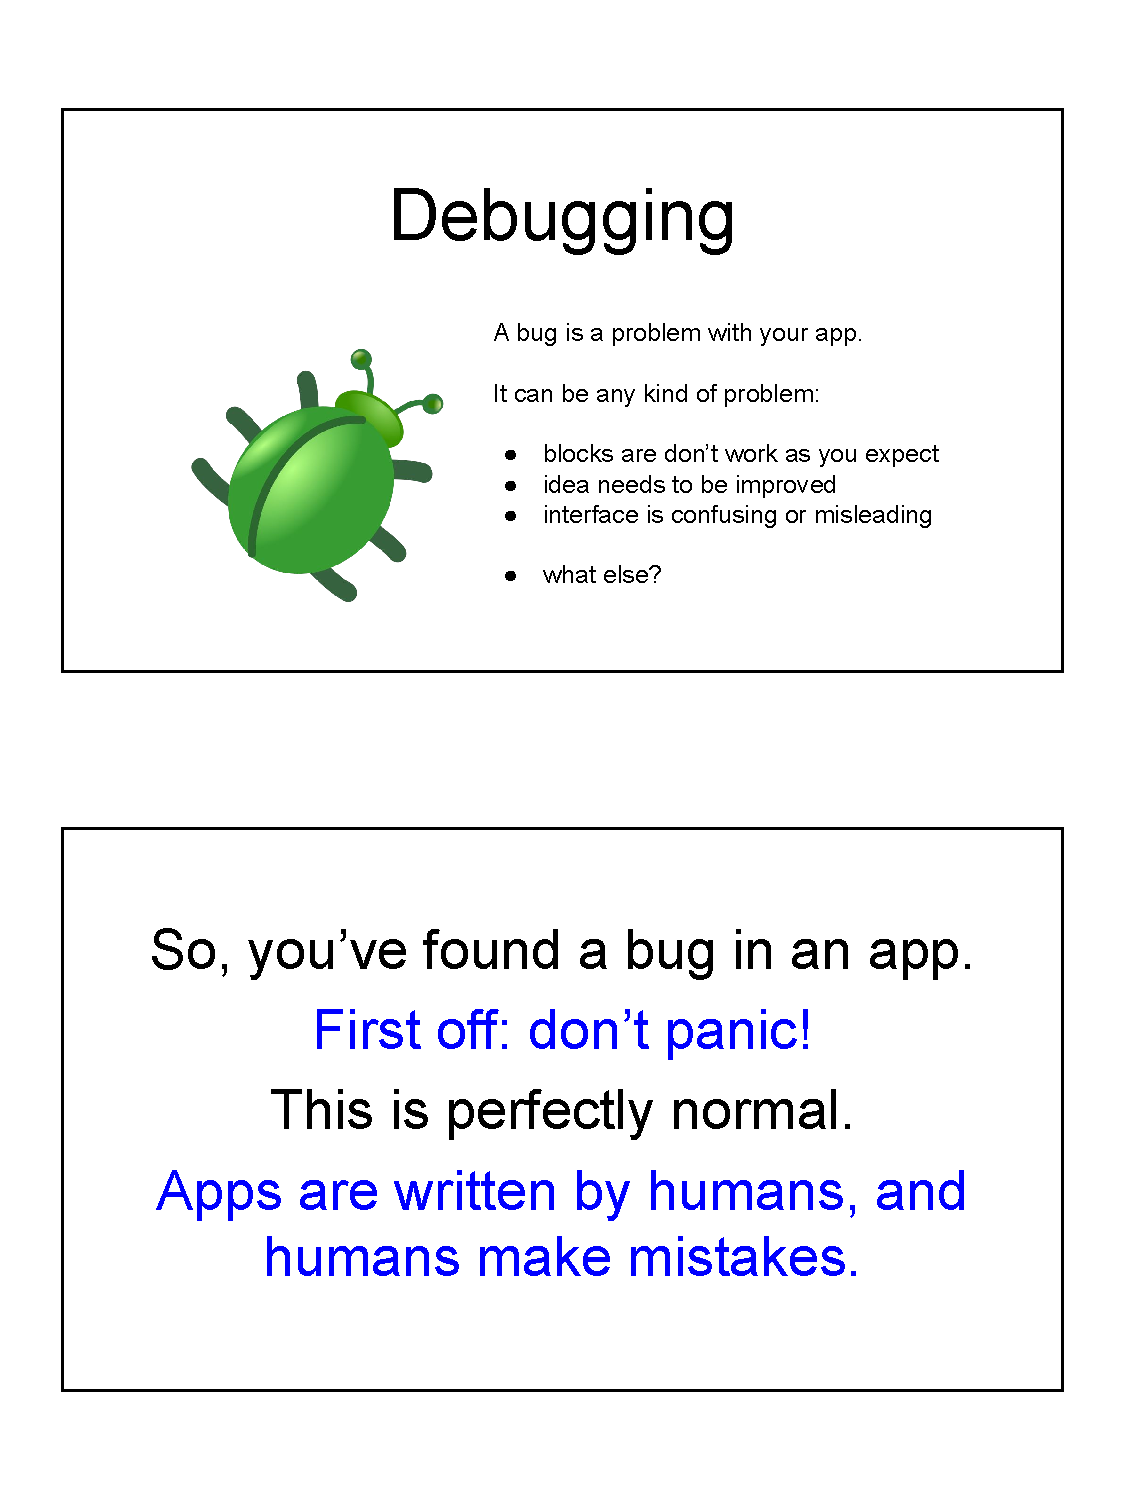
\includepdf[pages=-, frame, scale=.8]{IRB/Mark_Debugging_Lecture_handout.pdf}
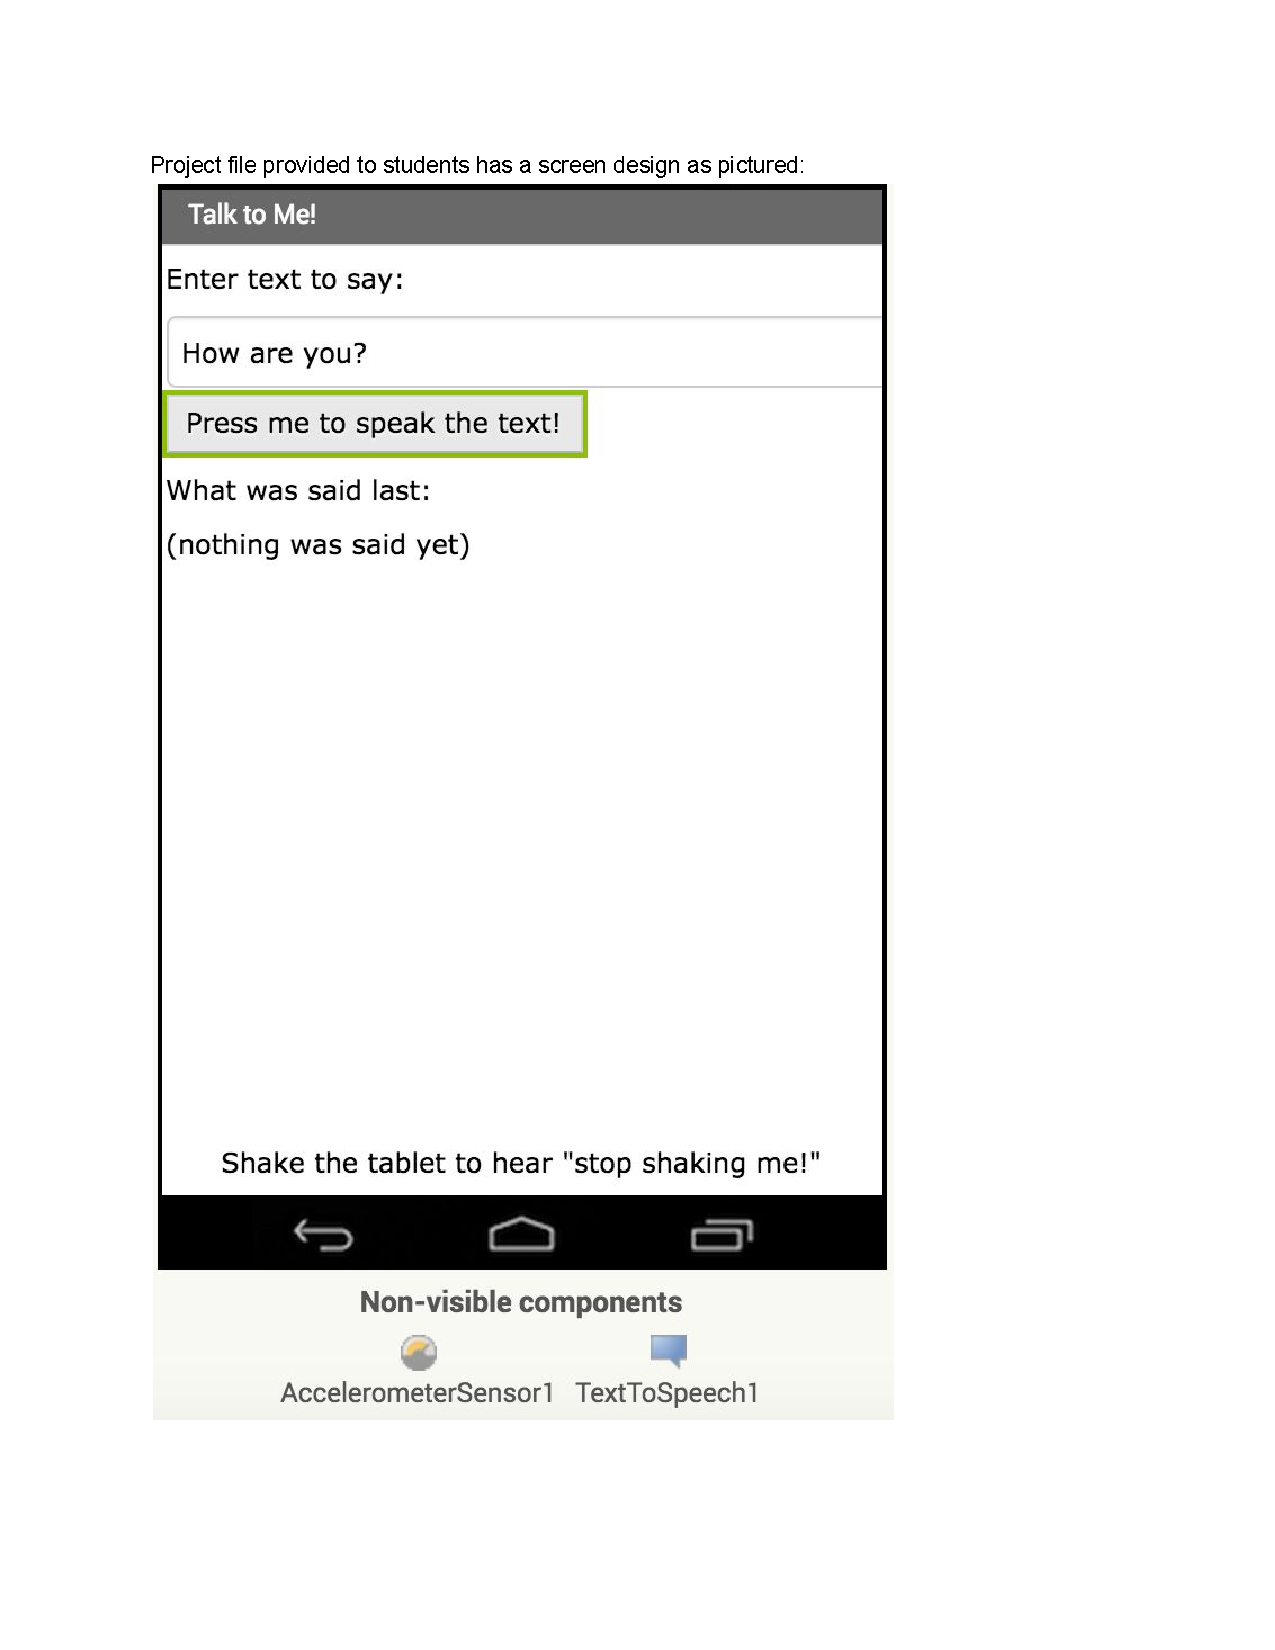
\includepdf[pages=-, frame, scale=.8]{IRB/AM10DebuggingAssessment.pdf}
\label{apx:debugging-protocol}

\section{Temperature Activity}
The temperature activity embedded assessment was conducted during the summer camp. The following pages include a description of the starter app and the student worksheet. This activity did not have a slide deck to accompany its scaffolding lecture, and one needs to be added for future implementations.
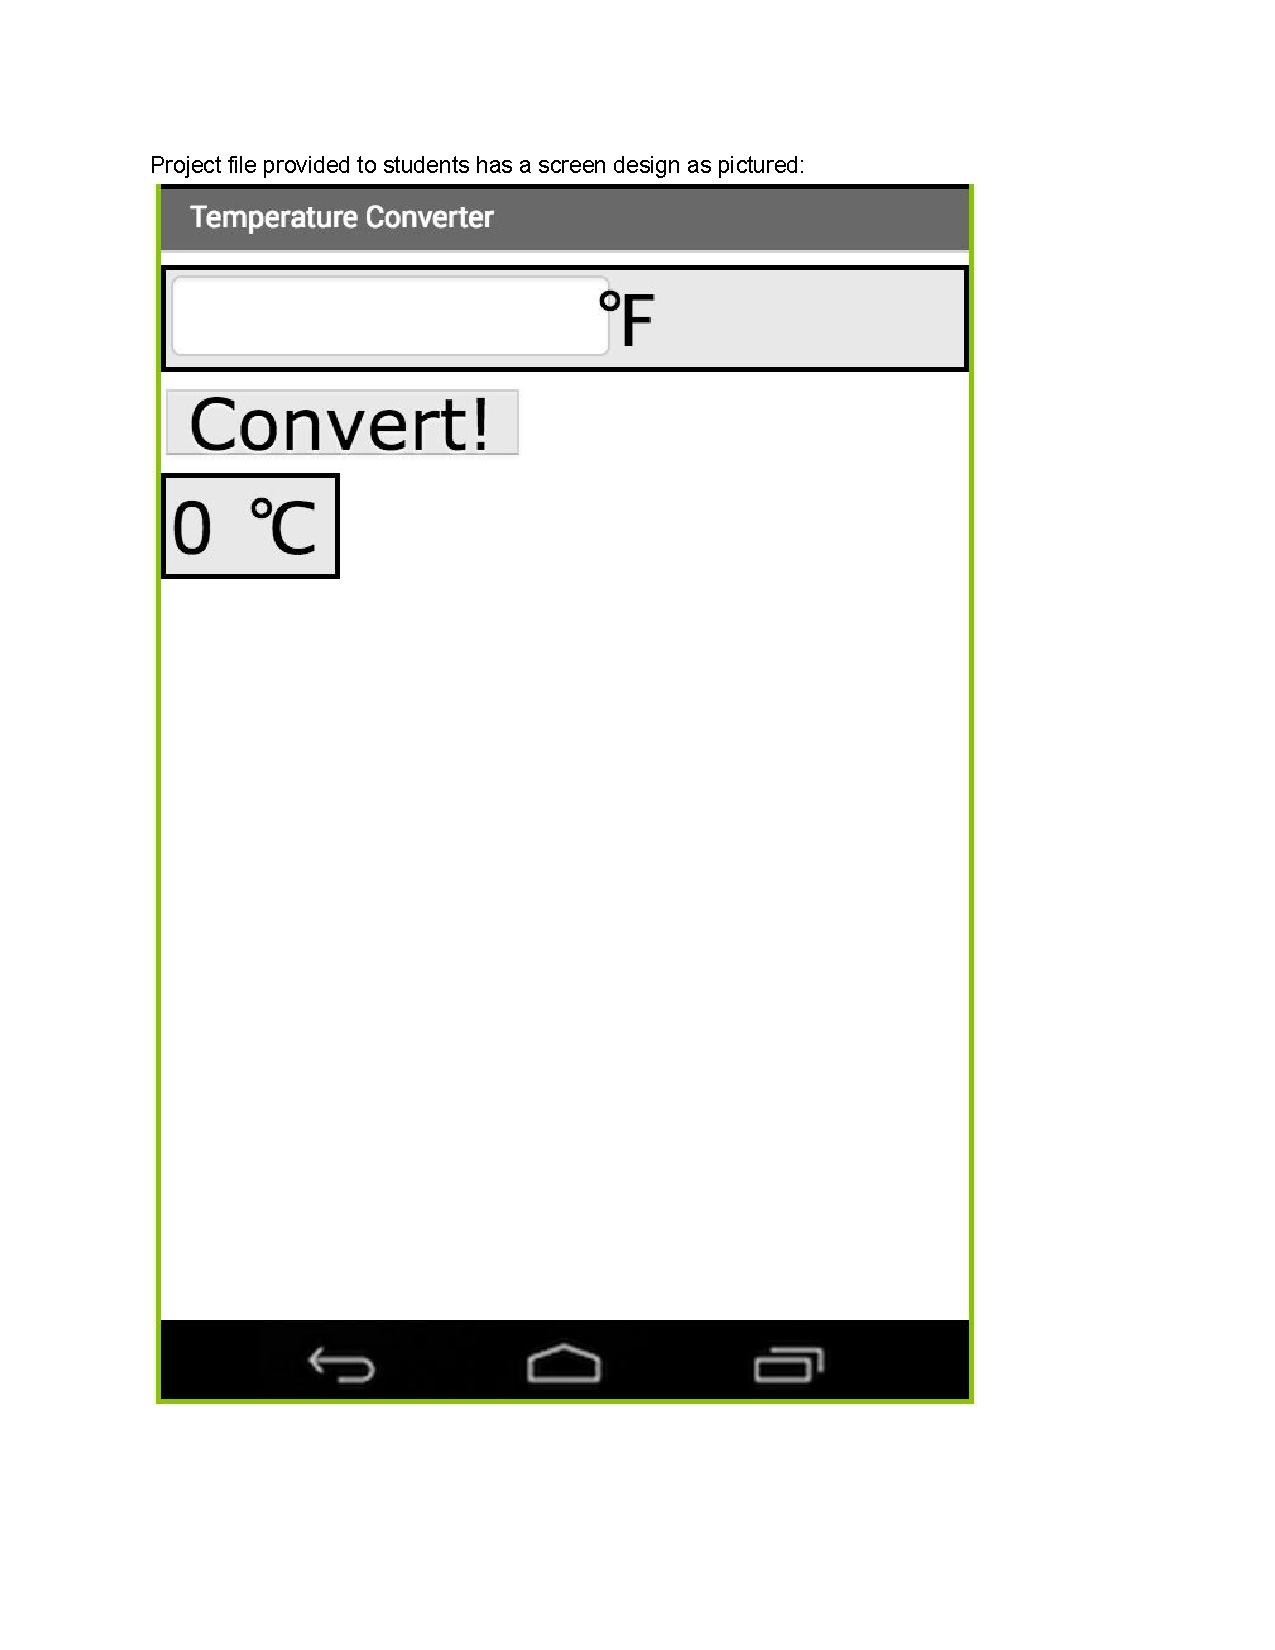
\includepdf[pages=-, frame, scale=.8]{IRB/AM10TemperatureAssessment.pdf}
\label{apx:temperature-protocol}

\chapter{Institutional Compliance Forms}
This project was monitored by the UMass Lowell Office of Institutional Compliance Institutional Review Board (IRB). This section contains the relevant submissions and approval letters between the research team and the IRB.

% \section{IRB Application}
% \label{IRB:app}
% "Middle School Pathways in Computer Science" was originally submitted by Fred Martin on June 25, 2014. Approval was received after expedited review on July 7, 2014, as IRB Protocol \# 14-144-MAR-XPD. The approval period was for July 7, 2014 through July 6, 2015.

% The following pages contain a copy of the IRB application form and the approval letter in response.

% 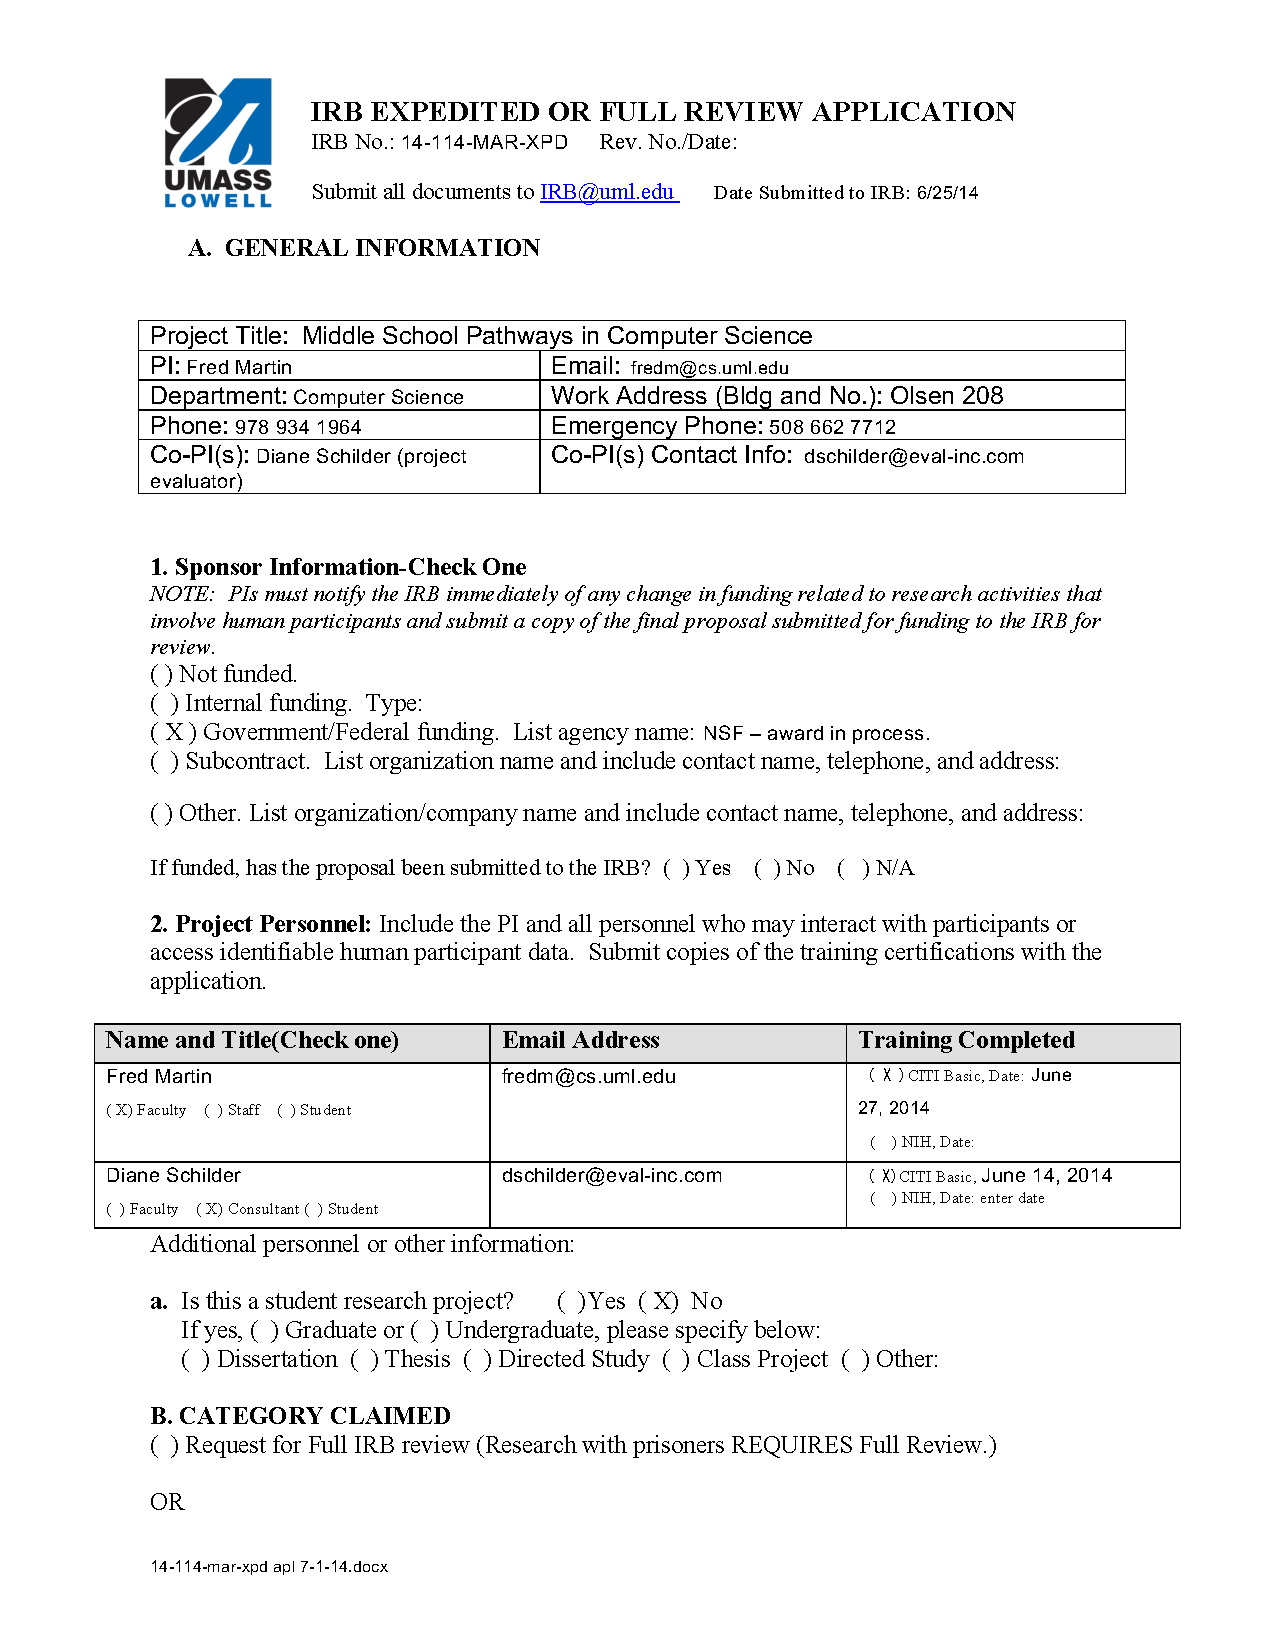
\includepdf[pages=-]{IRB/14-144-app.pdf}
% 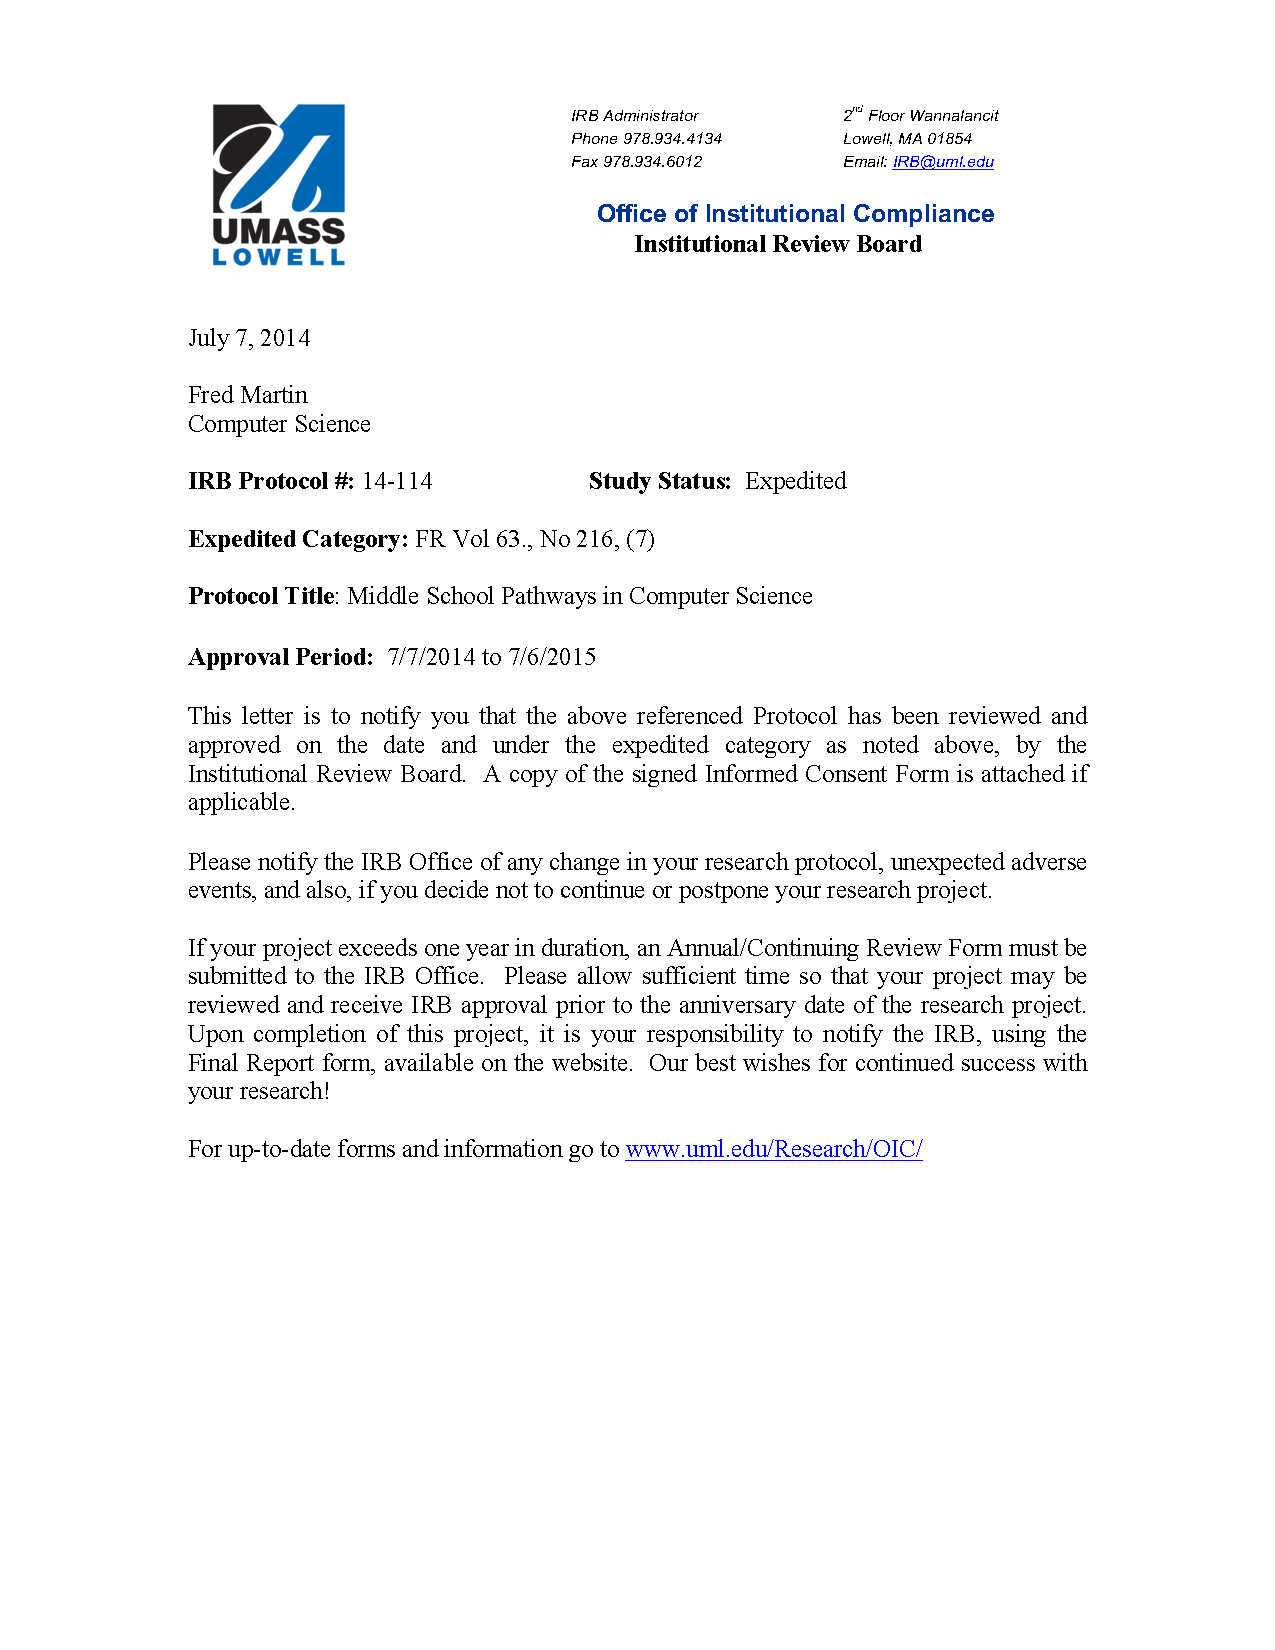
\includepdf[pages=-]{IRB/14-144-apv.pdf}

\section{The Debugging Activity and De-Identification Protocol}
This amendment added the author, Mark Sherman, and fellow researcher Lijun Ni to the project. This amendment also specified the Debugging Activity, and its protocol for classroom use. This amendment included the data de-identification protocol, which was discussed in Section \ref{sec:deident}.

The following pages contain the Debugging Game protocol description, including the de-identification protocol, a copy of the amendment application, and the approval letter.

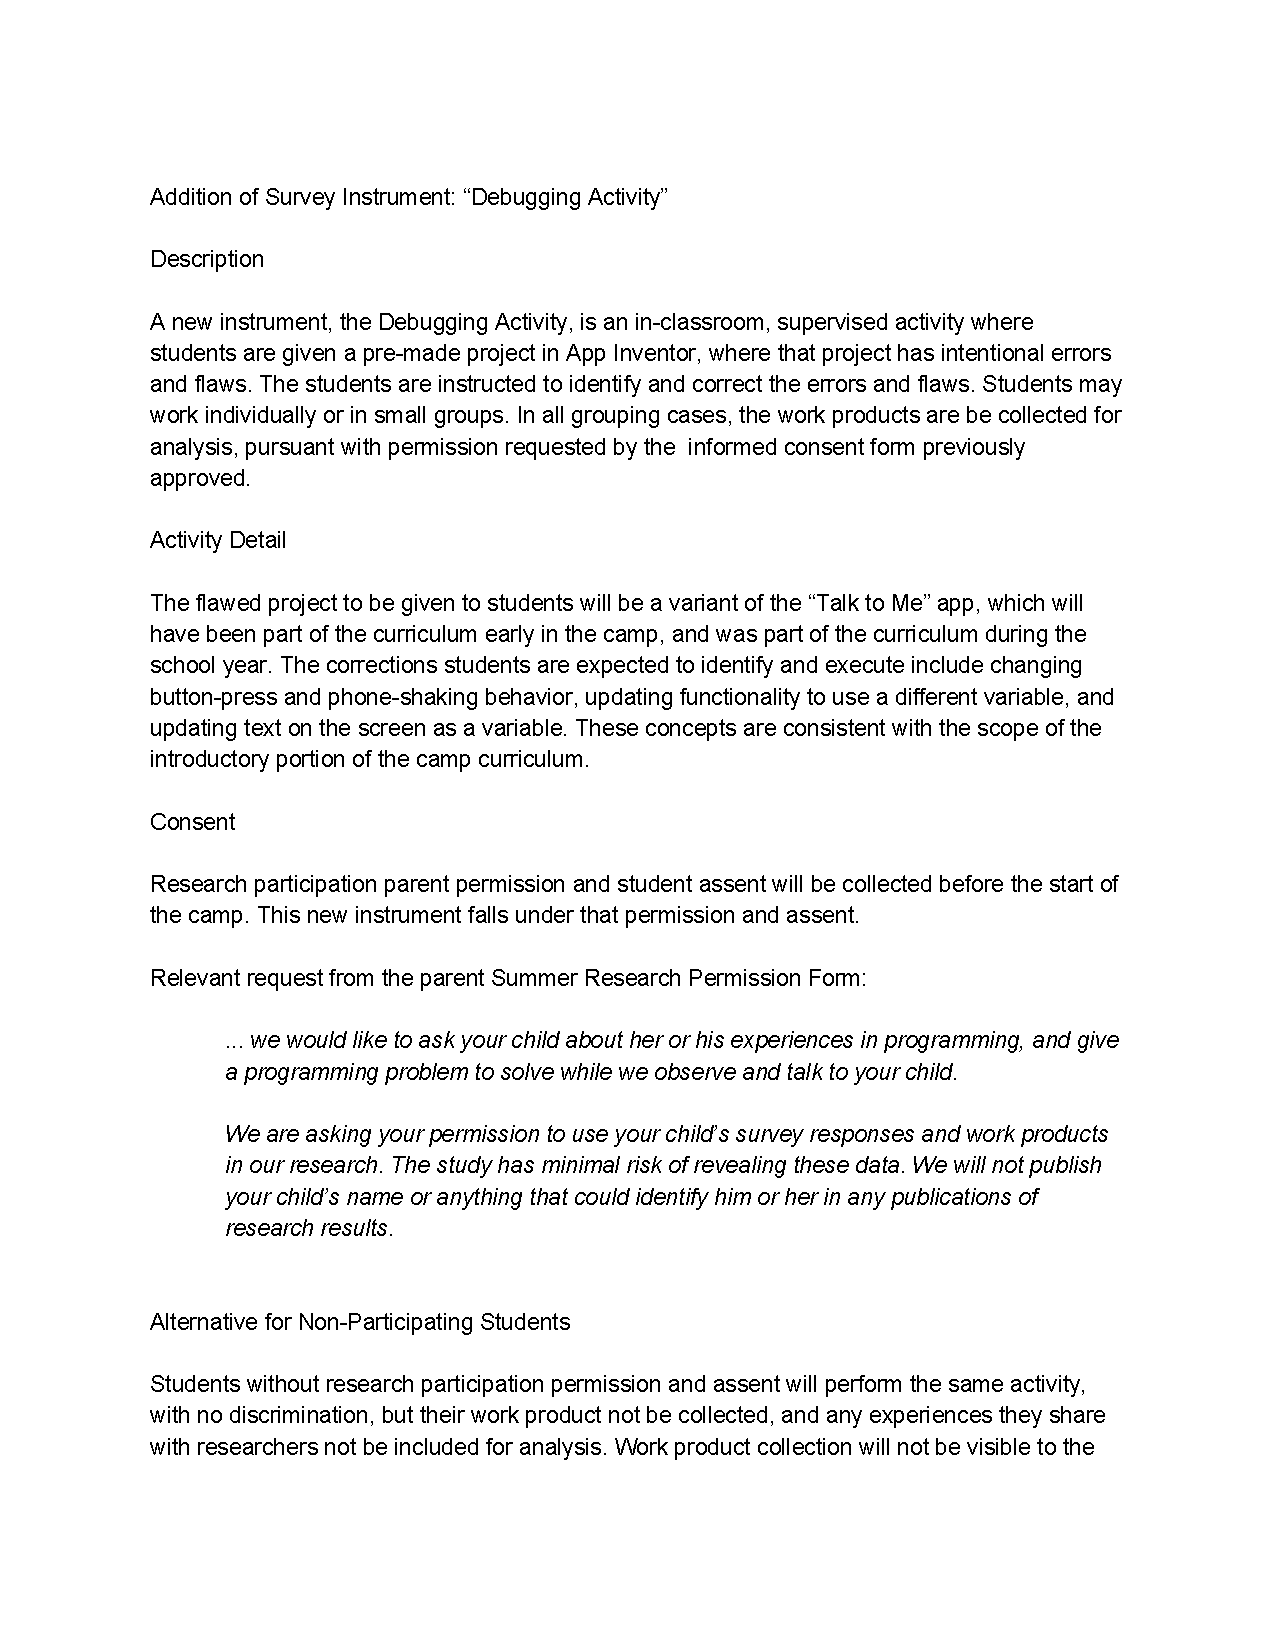
\includepdf[pages=-, frame, scale=.8]{IRB/AM2-DebuggingActivity2015.pdf}
%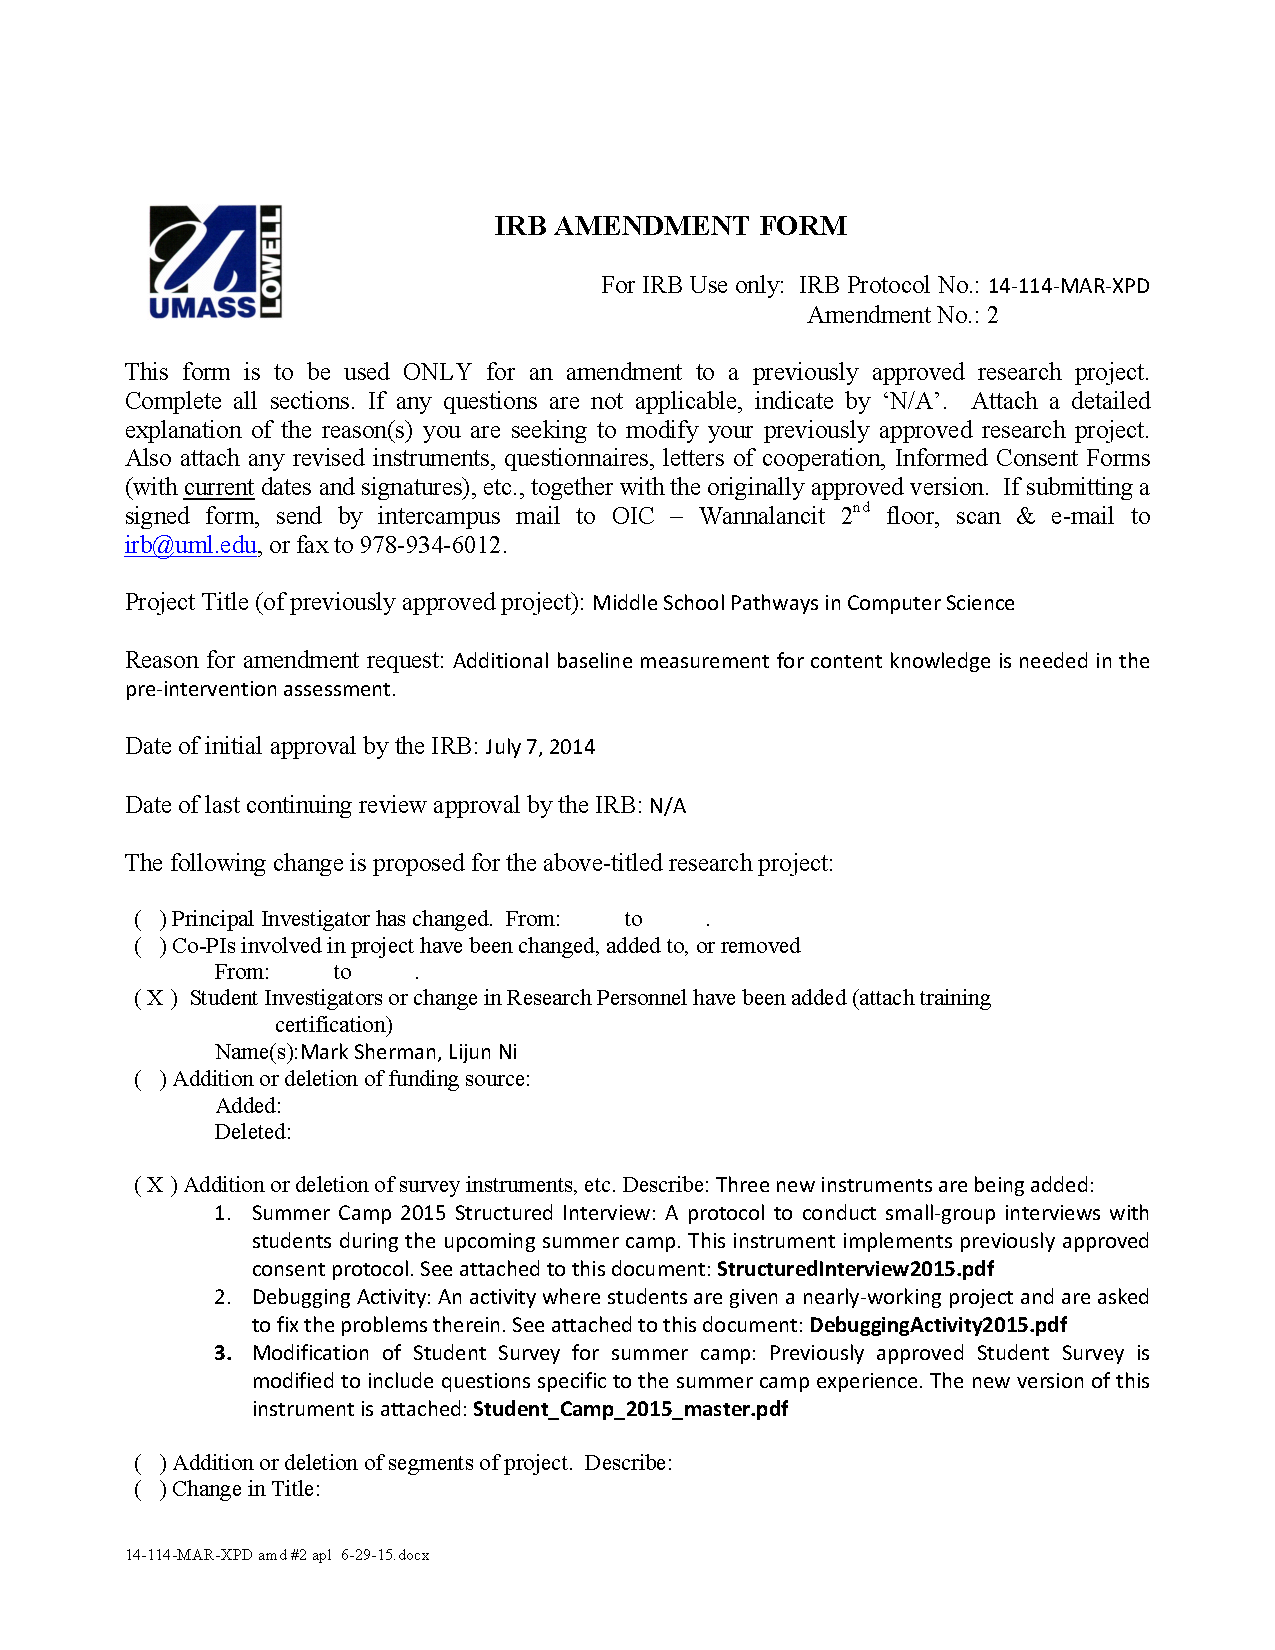
\includepdf[pages=-]{IRB/AM2-application.pdf}
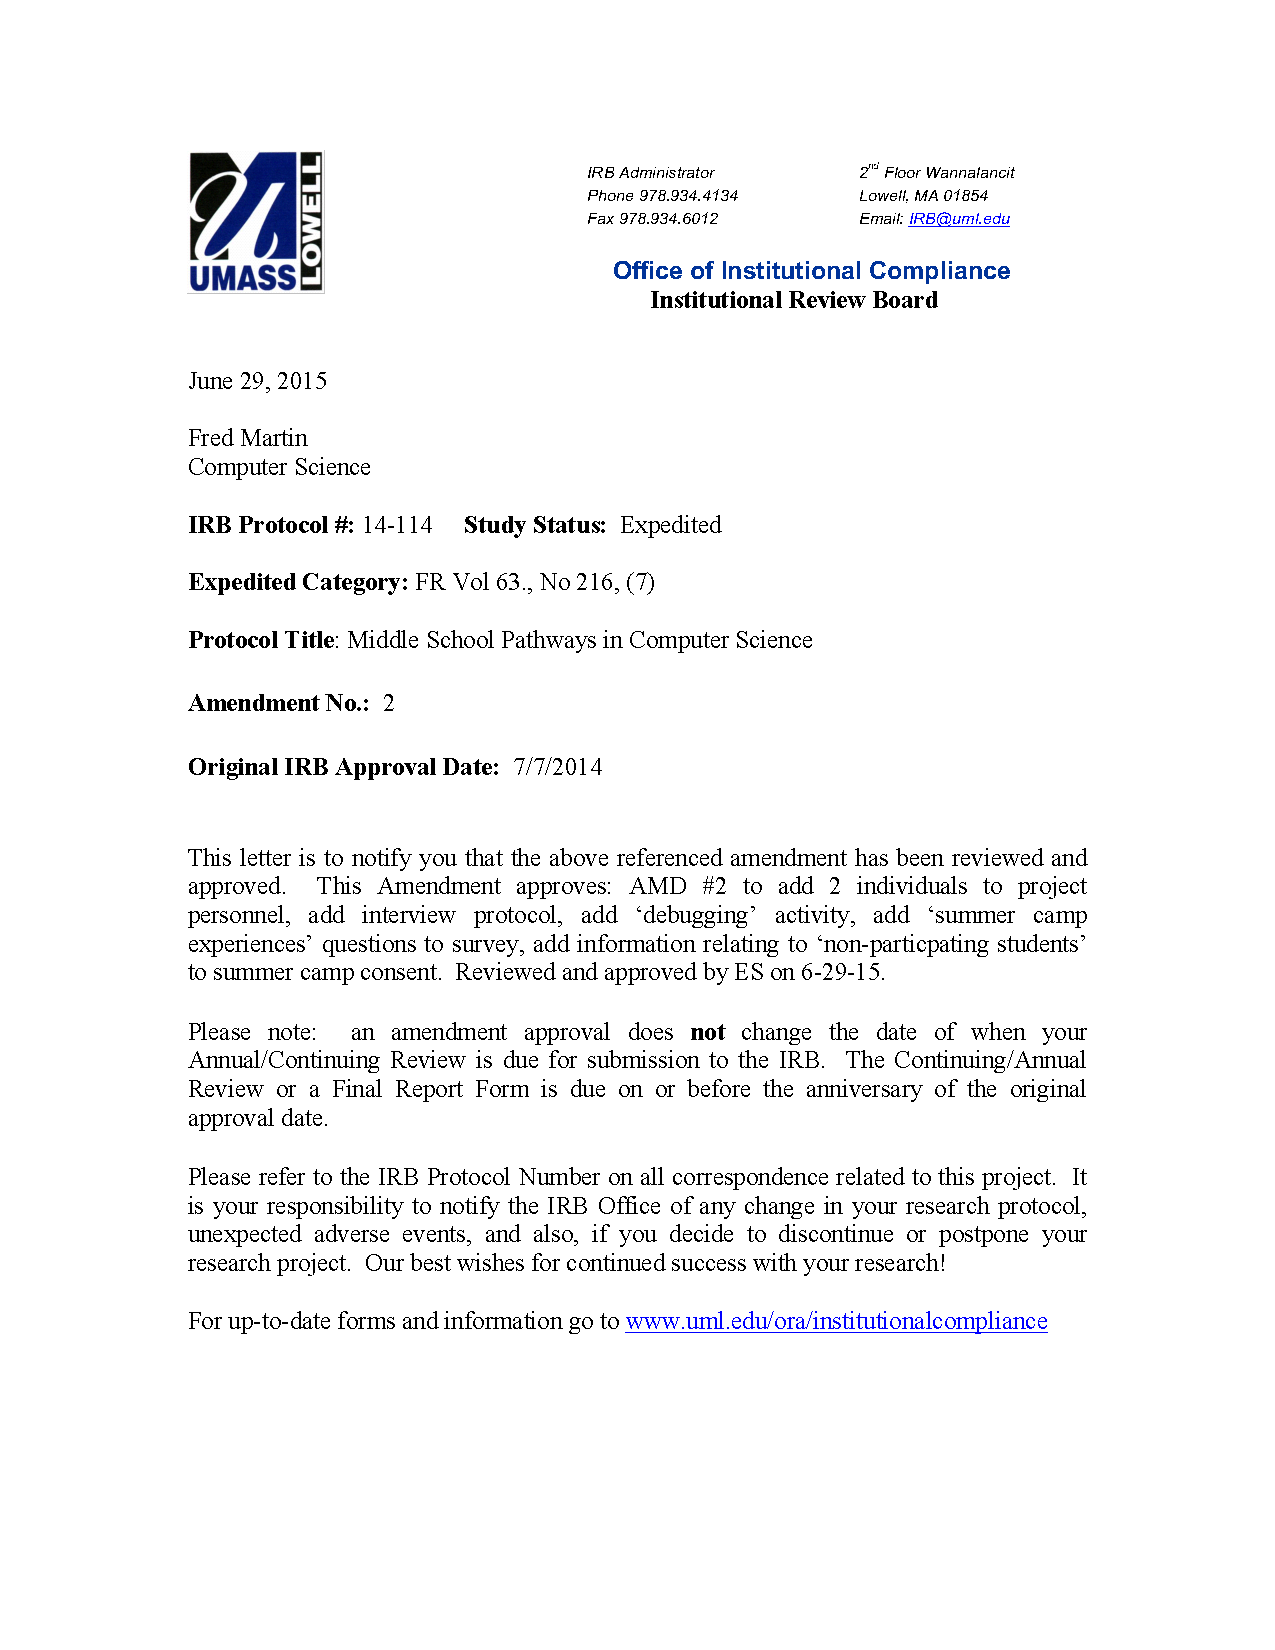
\includepdf[pages=-, frame, scale=.8]{IRB/AM2-approve.pdf}
\label{IRB:deident}


% \section{Annual/Continuing Review 2015}
% This application updated the IRB on the activities of the first year of the grant project, and declared intent for ongoing participant recruitment and data analysis until August 31, 2017. The following pages contain a copy of the review application and approval letter. The letter also mentions Amendment 3, which was approved at the same time, but is not relevant to the research in this document.

% 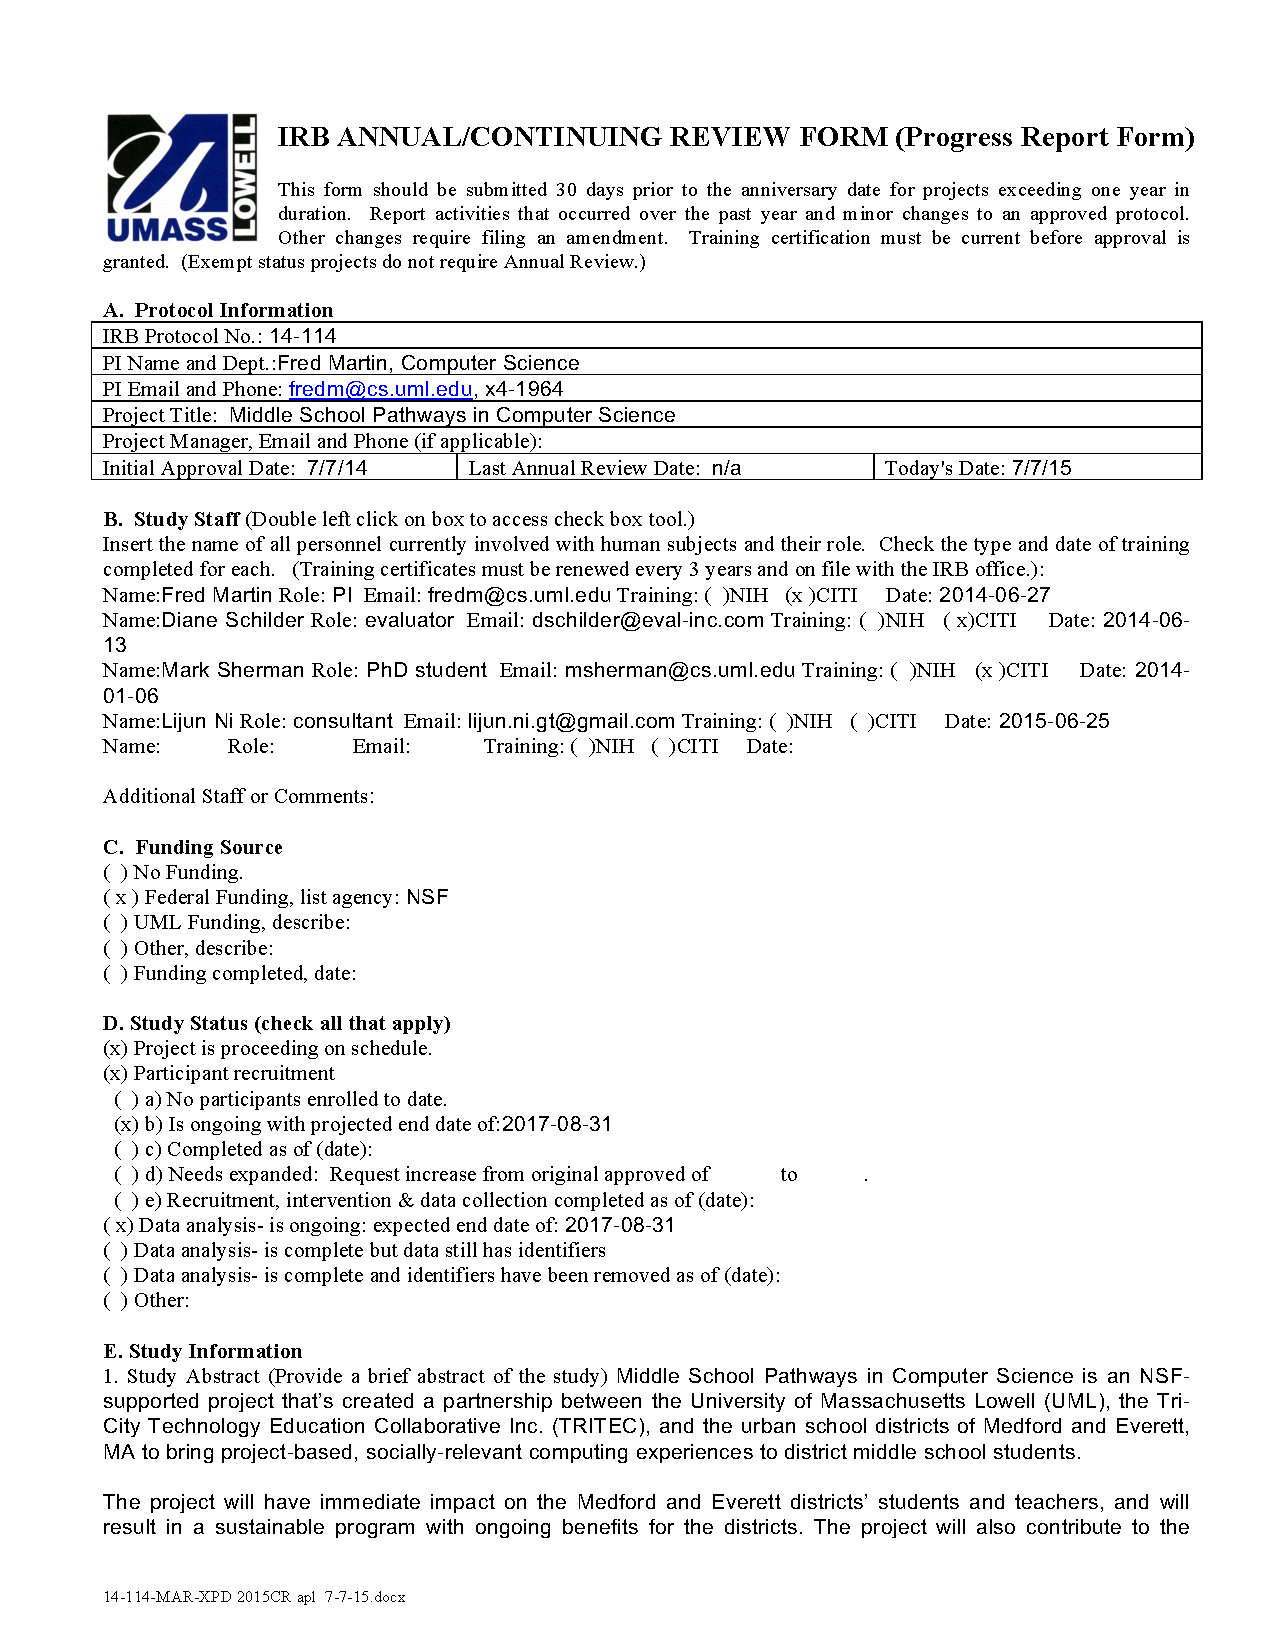
\includepdf[pages=-]{IRB/Year1-review-apl.pdf}
% 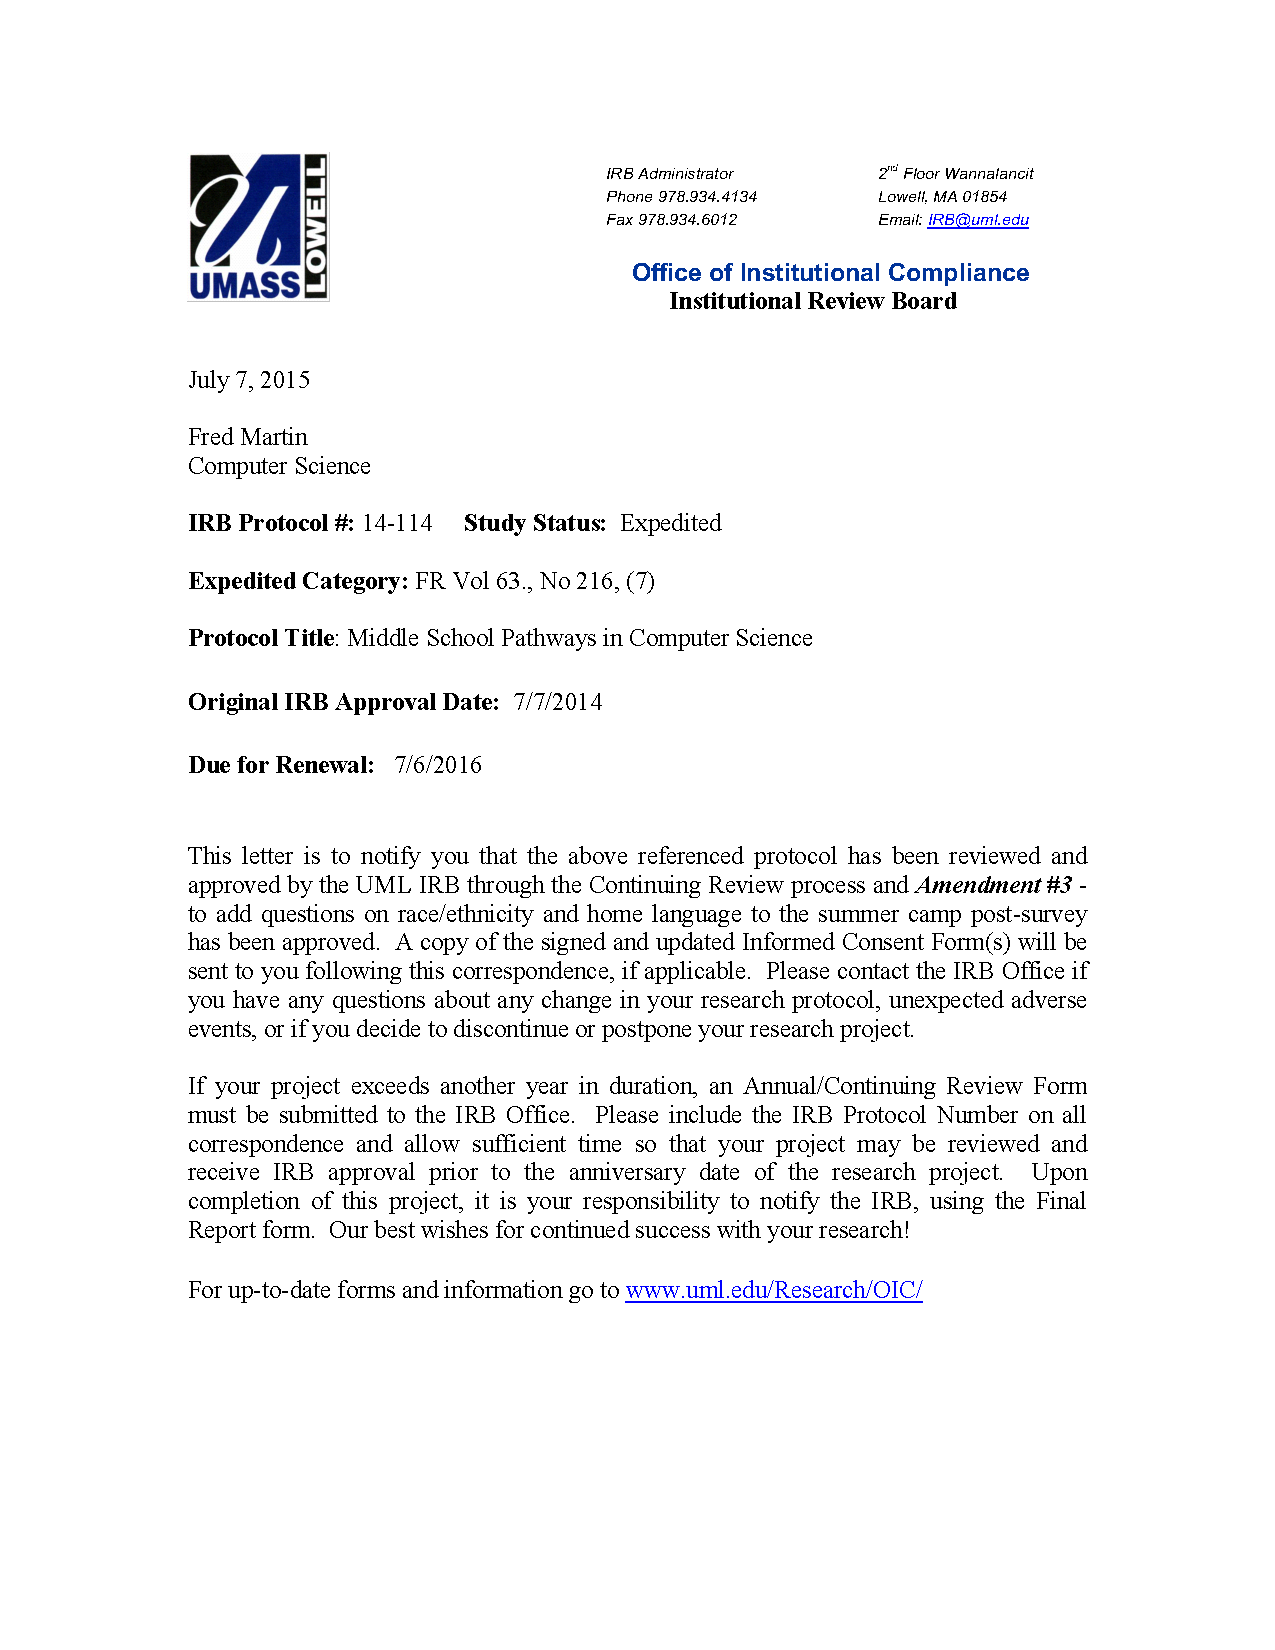
\includepdf[pages=-]{IRB/Year1-review-apv.pdf}

\section{Informed Consent, In-School}
\label{sec:icf:school}
The participants in this study were children, so an informed consent form was created for their parents, and a student assent form was provided to the children. The following pages are copies of those consent and assent forms as they were presented to the in-school cohort.

\includepdf[pages=-, frame, scale=.8]{IRB/icf-parent-in-school-rev3-9-14-15.pdf}
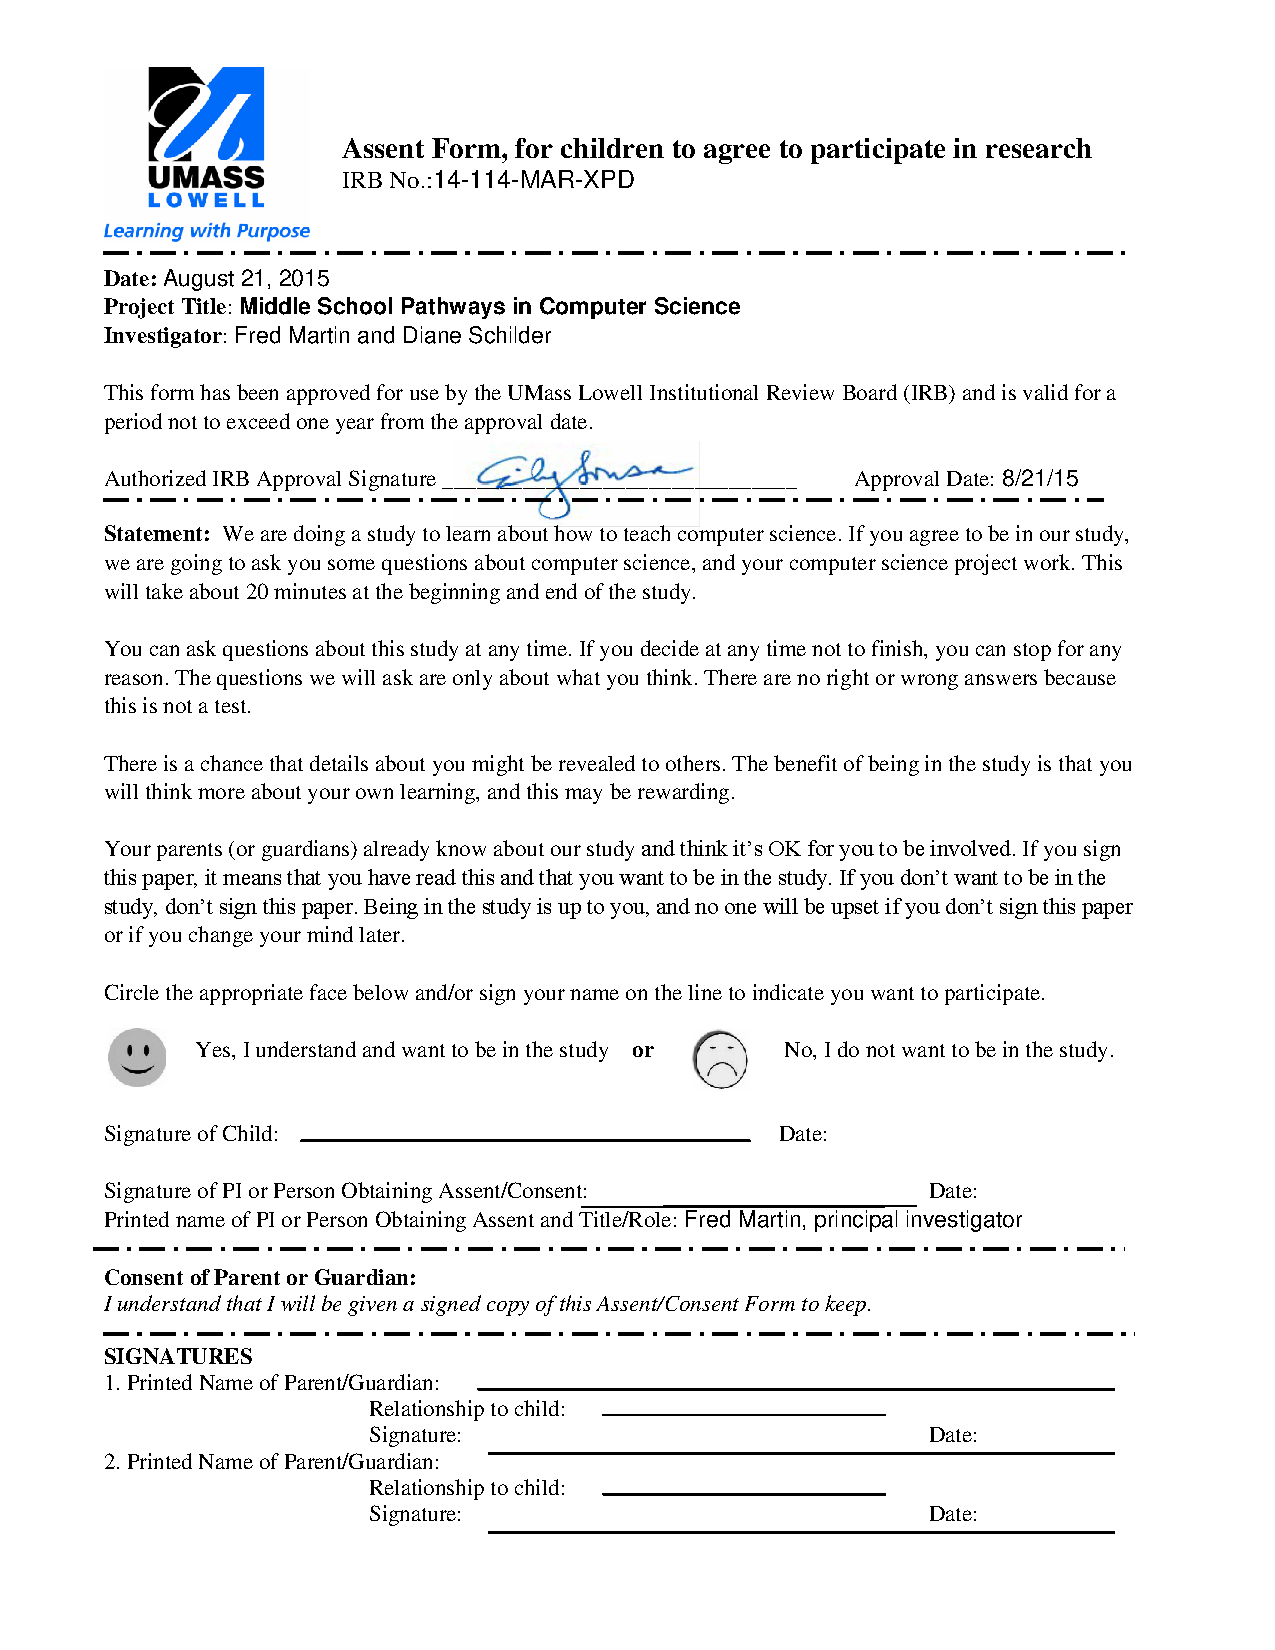
\includepdf[pages=-, frame, scale=.8]{IRB/icf-assent-8-21-15.pdf}


\section{Informed Consent, Summer Camp}
\label{sec:icf:camp}
The participants in this study were children, so an informed consent form was created for their parents, and a student assent form was provided to the children. The student assent form was unchanged from the In-School cohort (Appendix \ref{sec:icf:school}). The parental consent form was updated. The following pages are copies of the updated summer camp parental consent and the corresponding IRB approval letter.


\includepdf[pages=-, frame, scale=.8]{IRB/icf-summer-camp-parent-consent-2016.pdf}
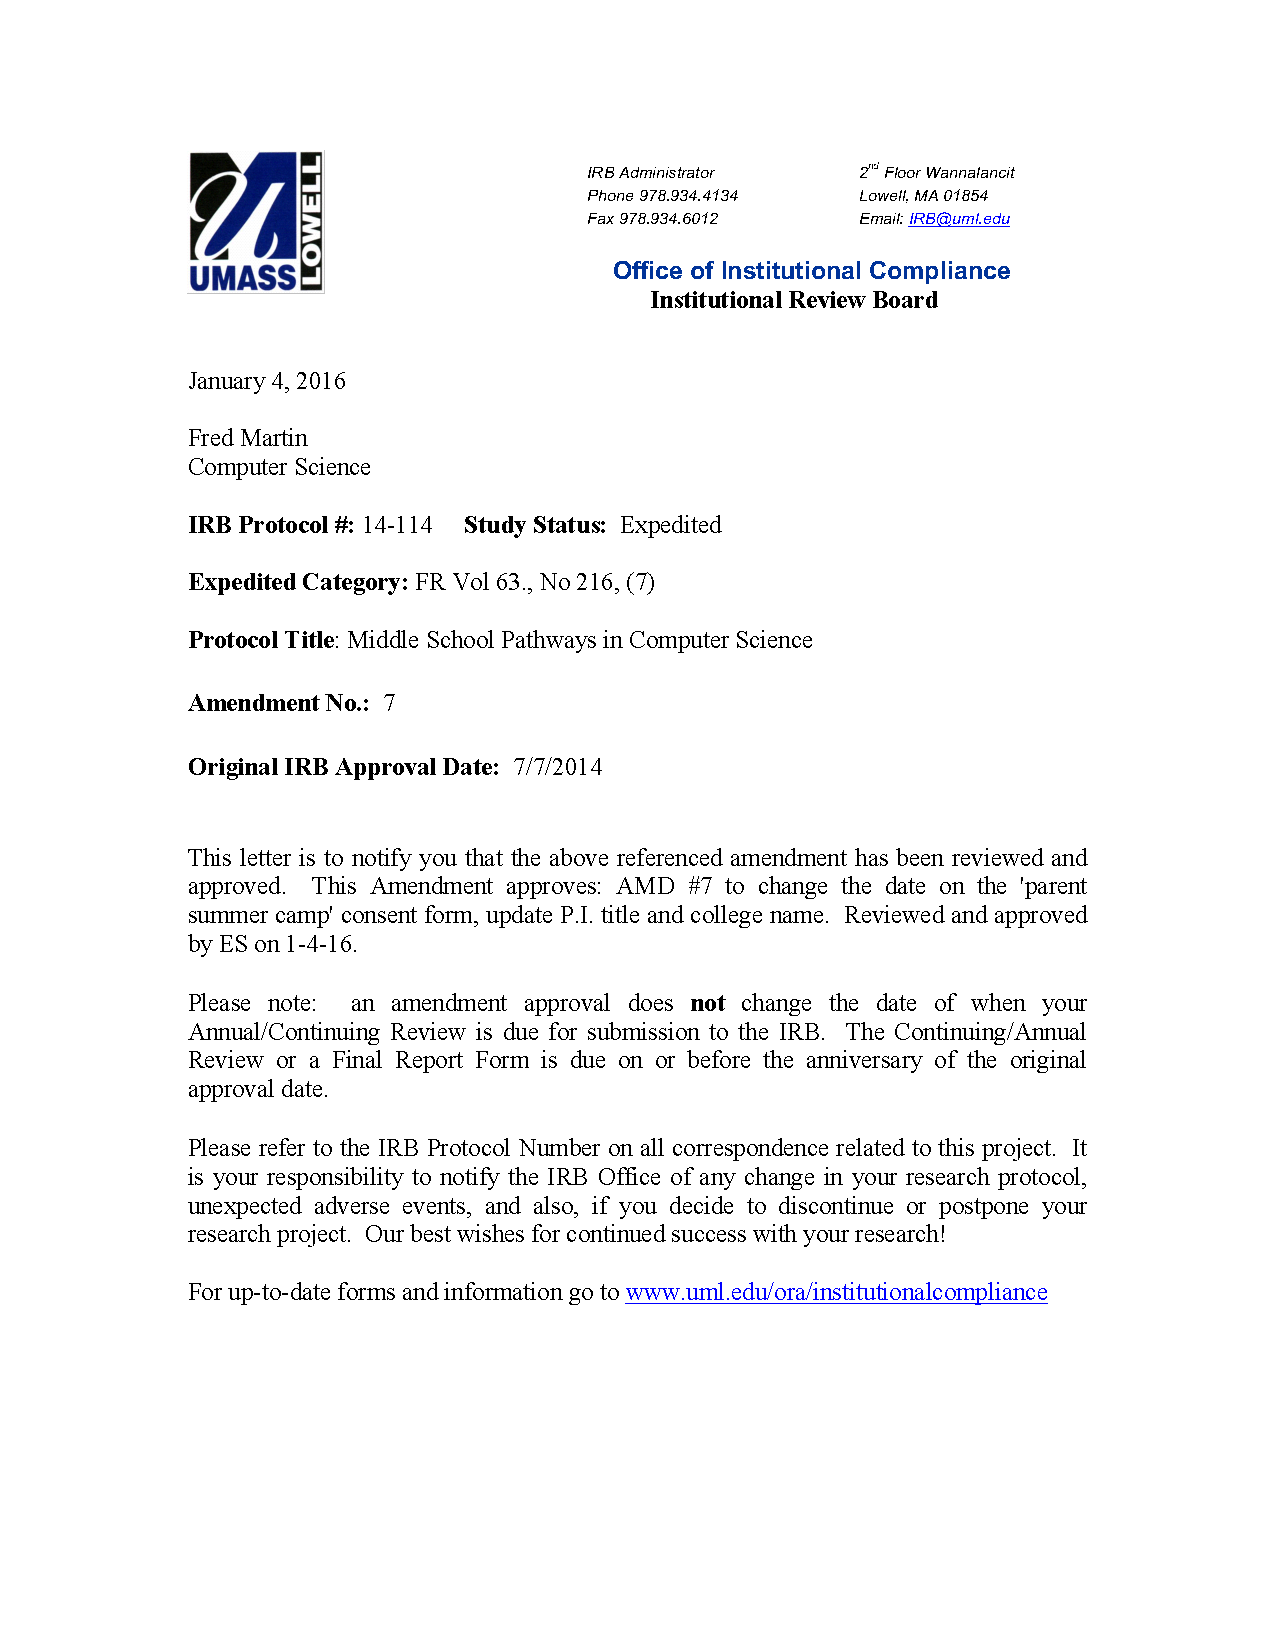
\includepdf[pages=-, frame, scale=.8]{IRB/icf-summer-camp-parent-consent-2016-approval.pdf}


% \section{Student Activities for Summer Camp Research}
% Amendment 10 added protocols for the Debugging Activity and Temperature Activity, both of which were used for data collection in this research. The protocol documents follow in Sections \ref{sec:IRB:debugging} and \ref{sec:IRB:temperature}, respectively. The following pages are copies of the IRB amendment form, and the approval letter affirming that these instruments operate under previously approved informed consent mechanisms. 

% 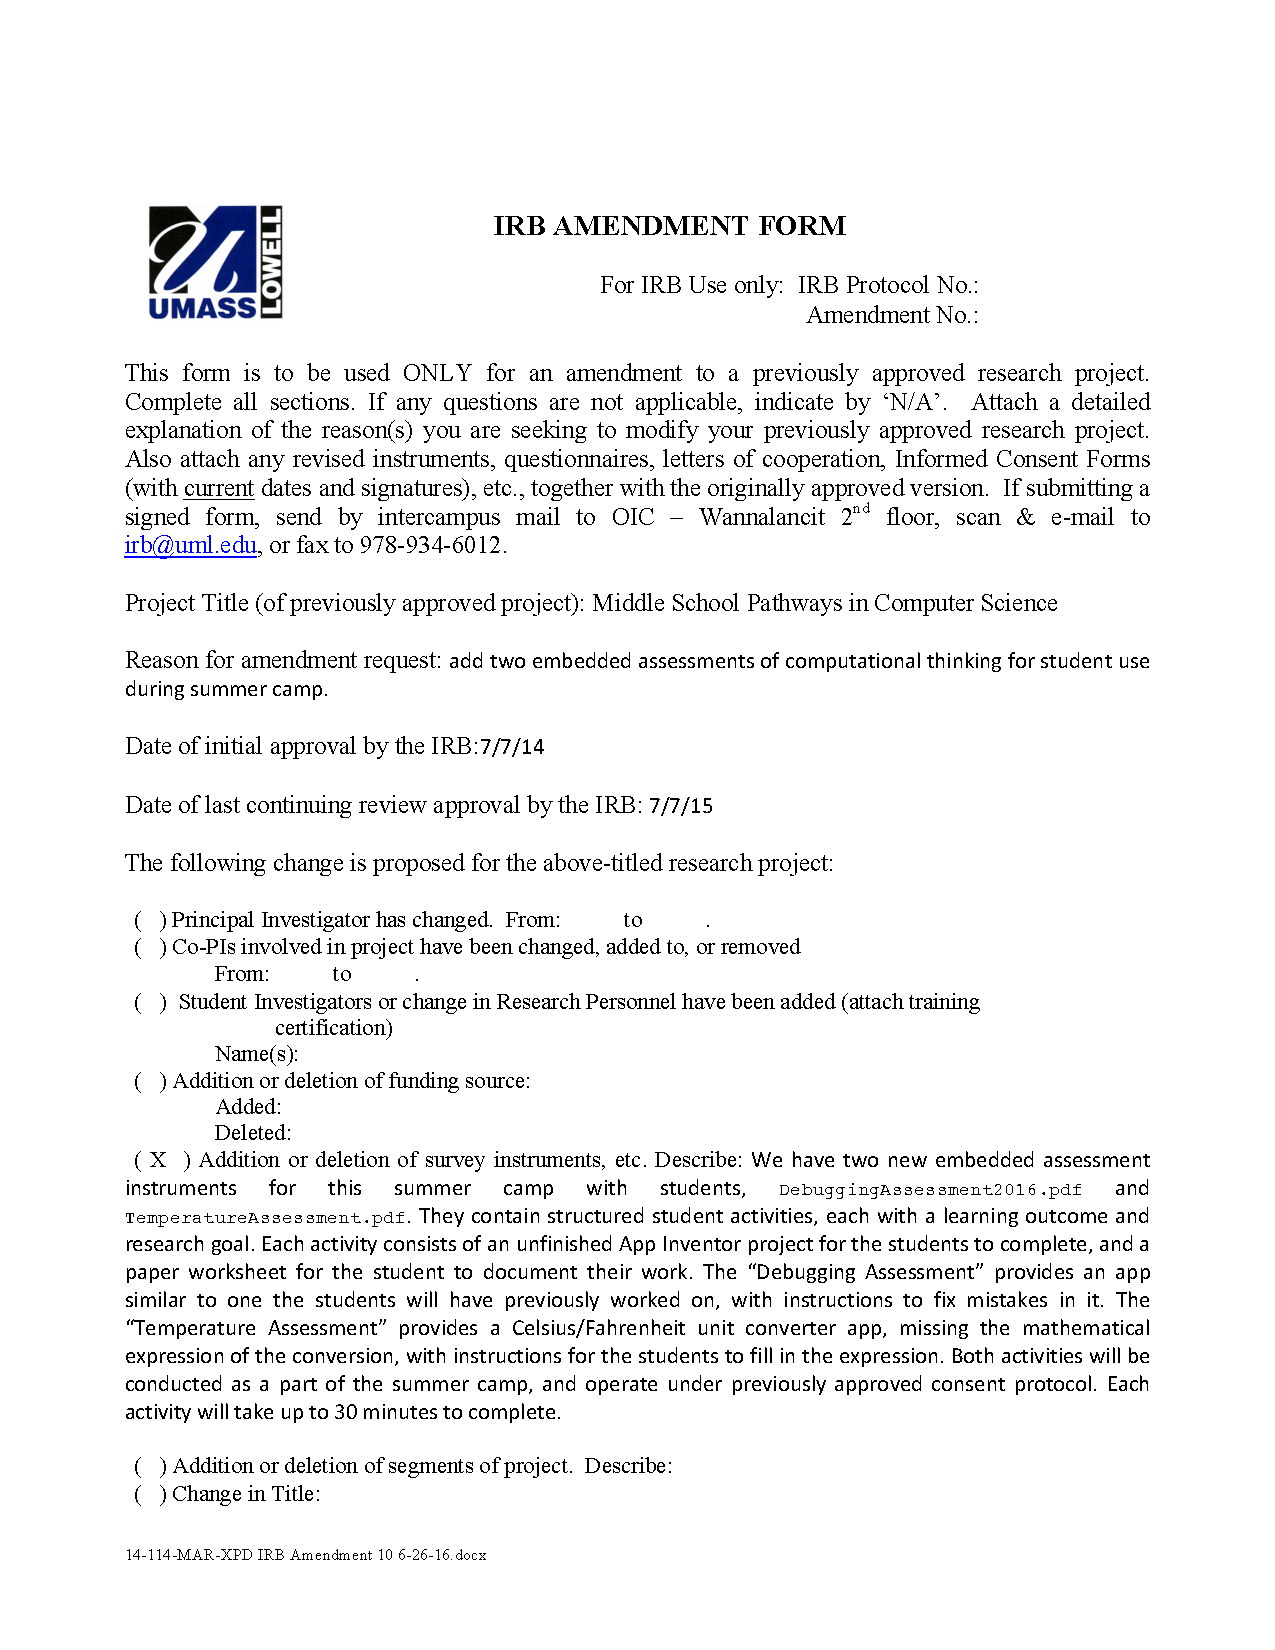
\includepdf[pages=-]{IRB/AM10-application.pdf}
% 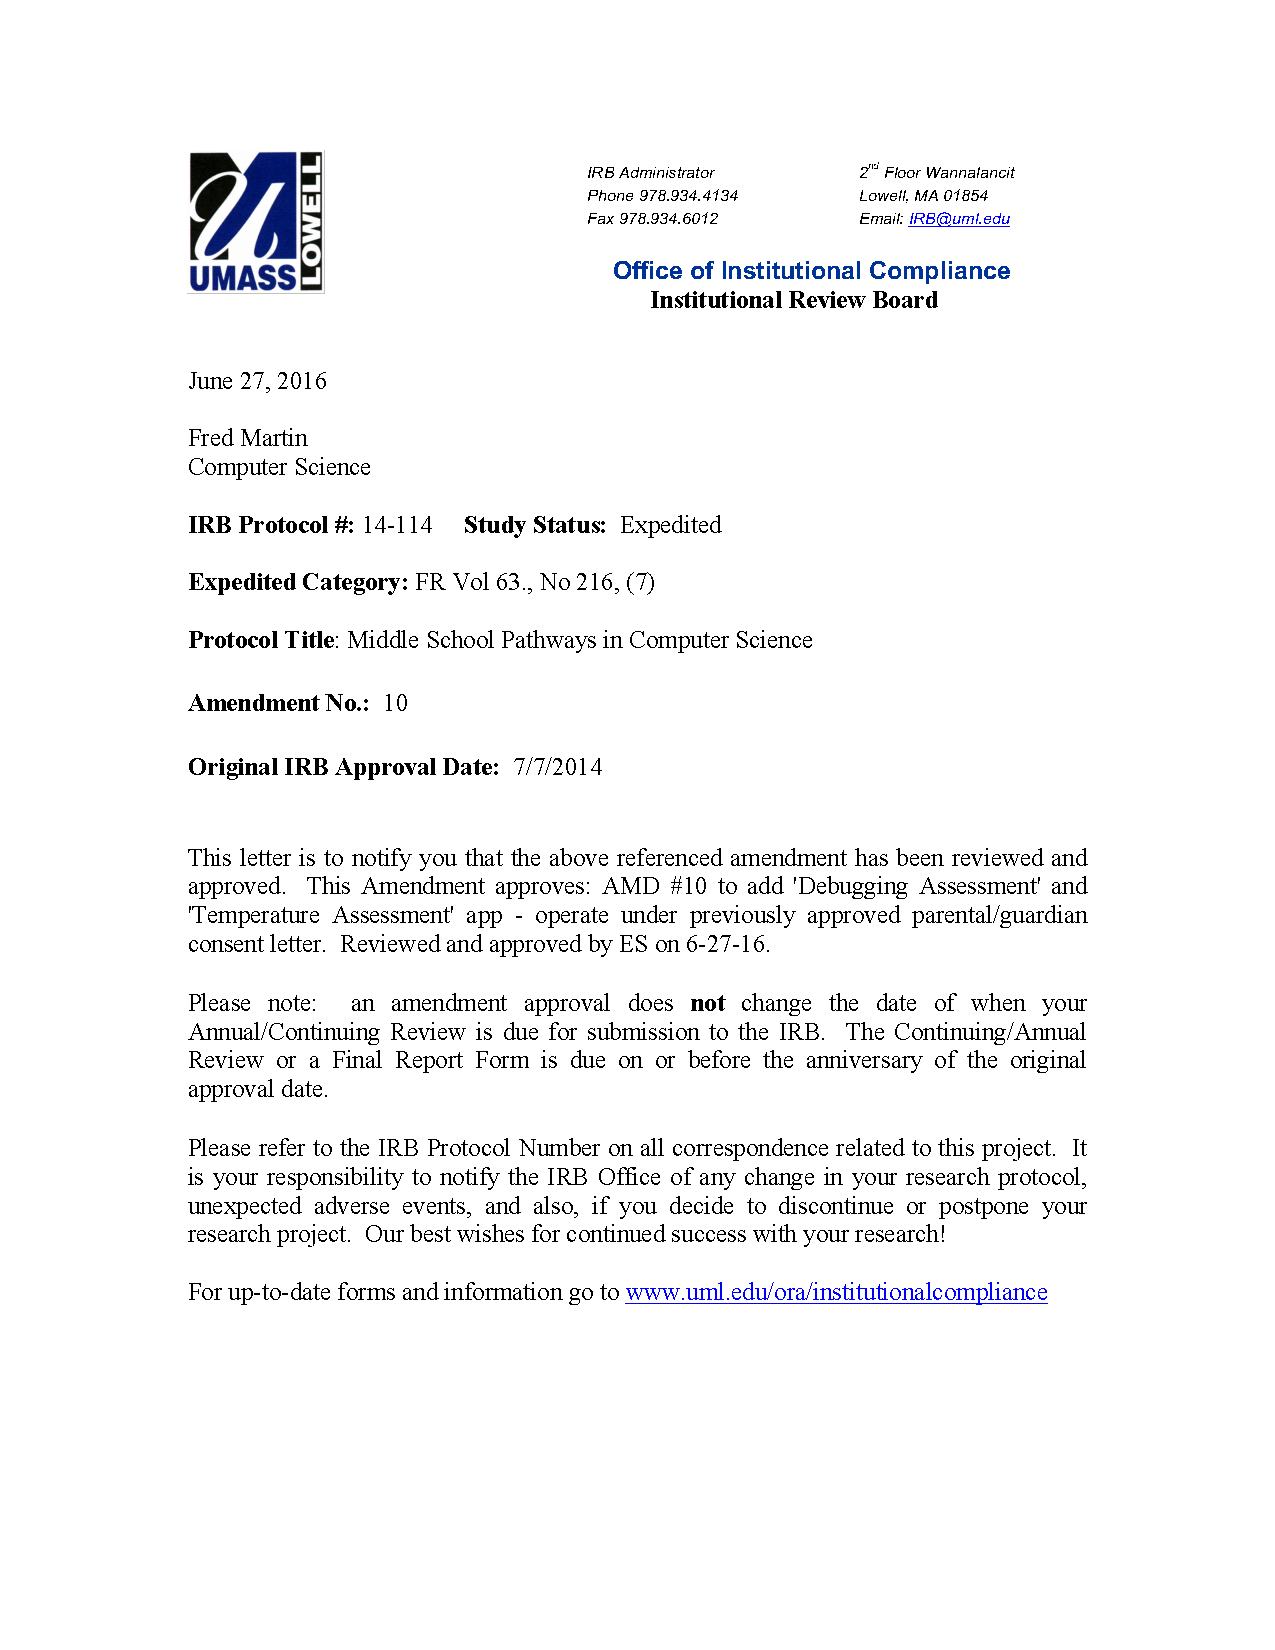
\includepdf[pages=-]{IRB/AM10-apv.pdf}

%%%%%%%%%%%%%%%%%%%%%%%%%%%%%%%%%%%%%%%%%%%%%%%%%%%%%%%%%%%%%%%%%%%%%%%%%%%%%%%%
%%%%%%%%%%%%%%%%%%%%%%%%%%%%%%%%%%%%%%%%%%%%%%%%%%%%%%%%%%%%%%%%%%%%%%%%%%%%%%%%

\chapter{Code Availability}

\noindent The App Inventor project, supported by the MIT Center for Mobile Learning, can be found here:

\noindent \url{https://github.com/mit-cml/appinventor-sources}

\noindent The modified version of App Inventor used in this project can be found in the author's github account:

\noindent \url{https://github.com/marksherman/appinventor-sources/tree/snapshot-service}

\noindent The long-term home for the features from this project is within the github home of the Engaging Computing Lab at UMass Lowell. That code can be found here:

\noindent \url{https://github.com/engaging-computing/appinventor-sources}

\noindent The source of this document is available from the author here:

\noindent \url{https://github.com/marksherman/umlthesis/tree/markphd}

\noindent The template used to write this document is available from the Engaging Computing lab at UMass Lowell:

\noindent \url{https://github.com/engaging-computing/umlthesis}

\noindent Especially relevant excerpts from the source code are listed in Appendix \ref{appendix:listings}.



\chapter{Author Biography}

Mark Sherman attended University of Massachusetts Lowell, earning a  Bachelor of Science degree in Computer \& Electrical Engineering, in 2008, demonstrating a capstone project in capacitive touchscreen technology. He continued his studies at UMass~Lowell, moving to the Computer Science department, and earned a Master of Science degree in Computer Science in 2010, with a research focus in computer science education. His masters thesis ``Exploration of Natural Design Tendencies of Novice Engineers'' identified testing and iteration patterns that may contribute to successful completion of engineering puzzles.

Mark is a proud member of the UMass Lowell Engaging Computing Group, where he has worked since 2008.

Mark also serves as an App Inventor Master Trainer with MIT, where he visits winning teams of a national design competition, trains students and teachers in App Inventor, programming, and project management to facilitate the teams production of a functional mobile application.

Mark has taught undergraduate courses at UMass Lowell, and led many teacher professional development trainings, including work in China and India, and many more in Massachusetts.



\end{document}
